\documentclass[11pt]{book}
\oddsidemargin 0in
\evensidemargin 0in
\marginparwidth 0in
\textheight 8in
\textwidth 6.5in
\topmargin 0in
\headheight 14pt
\usepackage{amssymb,amsmath,amsthm,fancyhdr,supertabular,longtable,hhline}
\usepackage{colortbl}
\usepackage{import, multicol,boxedminipage}
\usepackage{chapterfolder}
\usepackage[metapost,truebbox]{mfpic}
\usepackage[pdflatex]{graphicx}
\usepackage{makeidx}
\usepackage[colorlinks, hyperindex, plainpages=false, linkcolor=blue, urlcolor=blue, pdfpagelabels]{hyperref}
\usepackage[all]{hypcap}
\usepackage{cancel}
\usepackage{sectsty}
\usepackage{textcomp}
\allsectionsfont{\mdseries \scshape}
\definecolor{ResultColor}{gray}{0.9}
\theoremstyle{definition}  % this prevents the text in definitions, theorems, and corollaries from being italicized
\newtheorem{defn}{\sc Definition}[chapter]
\newtheorem{thm}{\sc Theorem}[chapter]
\newtheorem{cor}[thm]{\sc Corollary}
\newtheorem{eqn}{\sc Equation}[chapter]
\newtheorem{ex}{\sc Example}[section]
\newtheorem{fig}{\sc Figure}[chapter]
\setlength{\parindent}{0in}
\newcommand{\bbm}{\begin{boxedminipage}{6.41in}}
\newcommand{\ebm}{\end{boxedminipage}}
\usepackage{array}
\setlength{\extrarowheight}{2pt}
\allowdisplaybreaks[2]
\allsectionsfont{\mdseries \scshape}
%Below is for Helvetica (scaled): 
\usepackage[scaled=.92]{helvet}   
\renewcommand{\familydefault}{\sfdefault}  %makes the text of the book sans serif
\usepackage[helvet]{sfmath}  %makes the math in the book sans serif
\allsectionsfont{\sffamily}  %makes the chapter and section titles sans serif
\begin{document}
\newcounter{HW}
\newcounter{HWindent}
\renewcommand{\textinterrobang}{$! \! \! ?$}


\chapter{\sc The Conic Sections}

\section{Introduction to Conics}

\mfpicnumber{1}

\opengraphsfile{IntrotoConics}

\setcounter{footnote}{0}

\label{IntrotoConics}

In this chapter, we study the \index{conic sections ! definition} \textbf{Conic Sections} - literally `sections of a  cone'.  Imagine a double-napped cone as seen below being `sliced' by a plane. 

\centerline{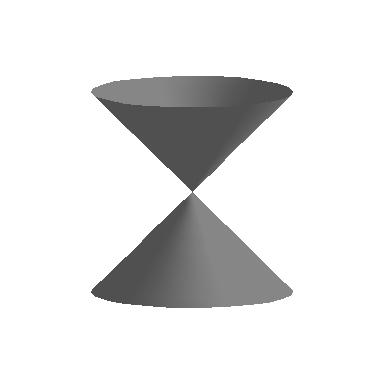
\includegraphics[width=2in]{./IntrotoConicsGraphics/cone.jpg}}

If we slice the cone with a horizontal plane the resulting curve is a \index{circle ! from slicing a cone} \textbf{circle}.

\begin{center}

\begin{tabular}{cc}

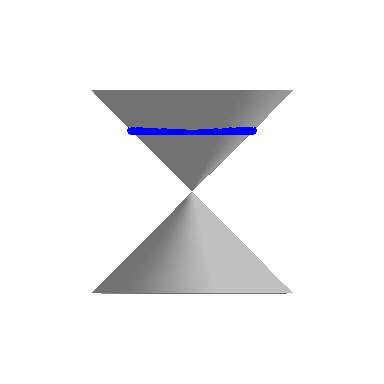
\includegraphics[width=2in]{./IntrotoConicsGraphics/Circle01.jpg} & 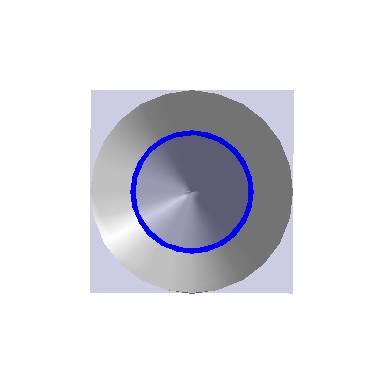
\includegraphics[width=2in]{./IntrotoConicsGraphics/Circle02.jpg} \\

\end{tabular}

\end{center}

\pagebreak

Tilting the plane ever so slightly produces an \index{ellipse ! from slicing a cone} \textbf{ellipse}.

\begin{center}

\begin{tabular}{cc}

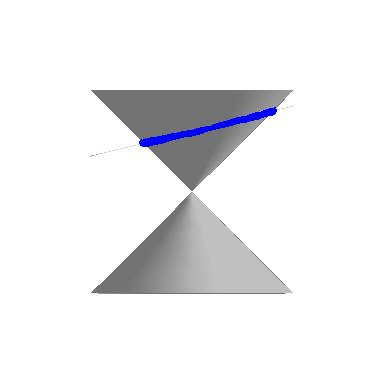
\includegraphics[width=2in]{./IntrotoConicsGraphics/Ellipse01.jpg} & 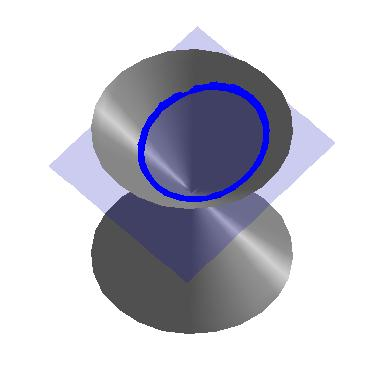
\includegraphics[width=2in]{./IntrotoConicsGraphics/Ellipse02.jpg} \\

\end{tabular}

\end{center}

If the plane cuts parallel to the cone, we get a \index{parabola ! from slicing a cone} \textbf{parabola}.

\begin{center}

\begin{tabular}{cc}

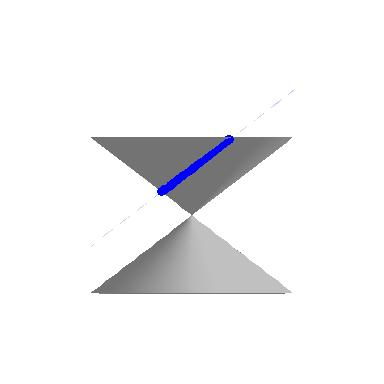
\includegraphics[width=2in]{./IntrotoConicsGraphics/Parabola01.jpg} & 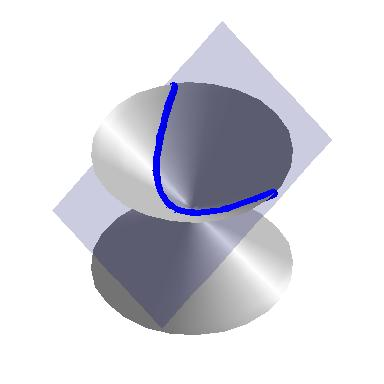
\includegraphics[width=2in]{./IntrotoConicsGraphics/Parabola02.jpg} \\

\end{tabular}

\end{center}

If we slice the cone with a vertical plane, we get a \index{hyperbola ! from slicing a cone} \textbf{hyperbola}.

\begin{center}

\begin{tabular}{cc}

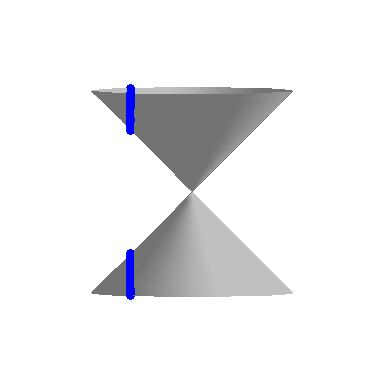
\includegraphics[width=2in]{./IntrotoConicsGraphics/Hyperbola01.jpg} & 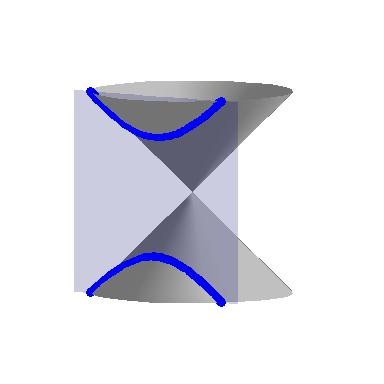
\includegraphics[width=2in]{./IntrotoConicsGraphics/Hyperbola02.jpg} \\

\end{tabular}

\end{center}


\pagebreak

If the slicing plane contains the vertex of the cone, we get the so-called `degenerate' conics:  a point, a line, or two intersecting lines.  

\phantomsection
\label{degenerateconics}

\begin{center}

\begin{tabular}{cc}

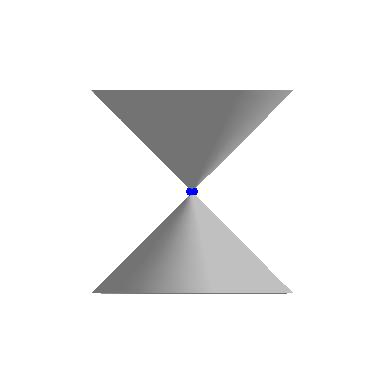
\includegraphics[width=2in]{./IntrotoConicsGraphics/Point01.jpg} & 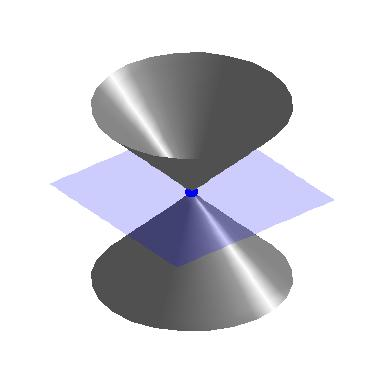
\includegraphics[width=2in]{./IntrotoConicsGraphics/Point02.jpg} \\


\includegraphics[width=2in]{./IntrotoConicsGraphics/Ilines01.jpg} & 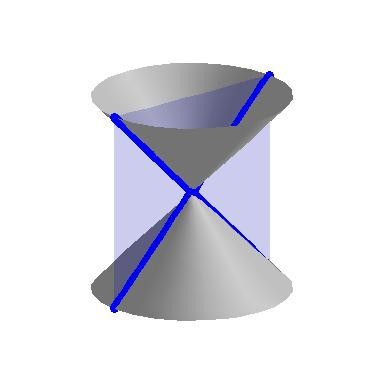
\includegraphics[width=2in]{./IntrotoConicsGraphics/Ilines02.jpg}\\

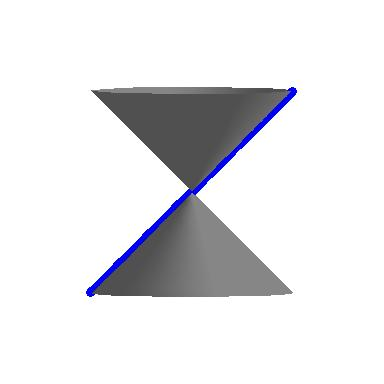
\includegraphics[width=2in]{./IntrotoConicsGraphics/Tline01.jpg} & 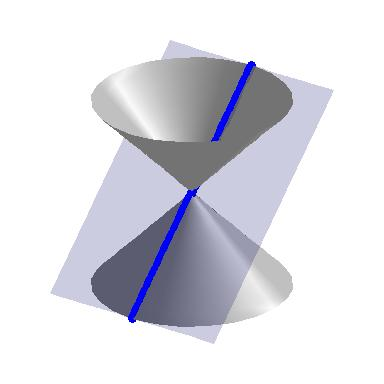
\includegraphics[width=2in]{./IntrotoConicsGraphics/Tline02.jpg} \\

\end{tabular}

\end{center}

\enlargethispage{.5in}
While this geometric introduction to the conic sections has its uses,\footnote{See Pierre Boulle's \textit{Planet of the Apes} for one example - we're serious!} in order to study the applications of the conic sections, we require a more analytic approach.  It turns out each of the  of the conic sections can be described as as a \textit{locus} of points - that is, a set of points which satisfy a certain condition involving distance.  The reader is referred to Section \ref{AppCartesianPlane} for a review of the distance and related formulas.

As we'll see, we'll be able to use the distance formula to algebraically represent the conic sections as  graphs of general quadratic equations in two variables.  That is, every conic section in the $xy$-plane can be represented as the graph of an equation of the form $Ax^2+Bxy+Cy^2+Dx+Ey +F = 0$ for real numbers $A$, $B$, $C$, $D$, $E$, and $F$.

\closegraphsfile

\newpage

\section{Parabolas}

\mfpicnumber{1}

\opengraphsfile{Parabolas}

\setcounter{footnote}{0}

\label{Parabolas}

We begin our study of the conic sections with parabolas, since we have already seen parabolas described as graphs of quadratic functions,  $f(x) = ax^2 + bx + c$ ($a \neq 0$).  It turns out that we can also describe parabolas in terms of distances.

\medskip

\colorbox{ResultColor}{\bbm

\begin{defn}

\label{paraboladefn}

Let $F$ be a point in the plane and $D$ be a line not containing $F$.   A \index{parabola ! definition of}  \textbf{parabola} is the set of all points equidistant from $F$ and $D$.  The point $F$ is called the \textbf{focus} \index{parabola ! focus} \index{focus (foci) ! of a parabola} of the parabola and the line $D$ is called the \textbf{directrix} \index{parabola ! directrix} \index{directrix ! of a parabola} of the parabola. 

\end{defn}

\ebm}

\medskip

Schematically, we have the following.

\begin{center}

\begin{mfpic}[15]{-7}{7}{0}{5}
\dashed \polyline{(0,2), (0,0), (0,-2)}
\dashed \polyline{(0,2), (2, 0.5), (2, -2)}
\dashed \polyline{(0,2), (-2,0.5), (-2, -2)}
\dashed  \polyline{(0,2), (4,2), (4, -2)}
\dashed  \polyline{(0,2), (-4,2), (-4, -2)}
\dashed \polyline{(0,2), (6,4.5), (6, -2)}
\dashed  \polyline{(0,2), (-6,4.5), (-6, -2)}
\plotsymbol[3pt]{Asterisk}{(0, 2)}
\tlabel[cc](6.5, -2.5){$D$}
\tlabel[cc](0, 2.5){$F$}
\arrow \reverse \arrow \function{-6.5, 6.5, 0.1}{-2}
\penwd{1.25pt}
\arrow \reverse \arrow \function{-6.25,6.25,0.1}{(x**2)/8}
\point[4pt]{(0,0)}
\point[4pt]{(2,0.5)}
\point[4pt]{(-2,0.5)}
\point[4pt]{(4,2)}
\point[4pt]{(-4,2)}
\point[4pt]{(6,4.5)}
\point[4pt]{(-6,4.5)}
\tlabel[cc](0.5,-0.5){$V$}
\end{mfpic}

\end{center}

Each dashed line from the point $F$ to a point on the curve has the same length as the dashed line from the point on the curve to the line $D$.  The point suggestively labeled $V$ is, as you may expect, the \textbf{vertex}.  The \index{parabola ! vertex} \index{vertex ! of a parabola} vertex is the point on the parabola closest to the focus.  

\smallskip

We want to use only the distance definition of parabola to derive the equation of a parabola and, if all is right with the universe, we should get an expression much like those studied in Section \ref{QuadraticFunctions}.  


\smallskip

For simplicity, assume that the vertex is $(0,0)$ and that the parabola opens upwards.  Let $p$ denote the directed\footnote{We'll talk more about what `directed' means later.} distance from the vertex to the focus, which by definition is the same as the distance from the vertex to the directrix.   Hence, the focus is $(0,p)$ and the directrix is the line $y = -p$.  Our picture becomes 

\begin{center}

\begin{mfpic}[15]{-7}{7}{0}{5}
\axes
\plotsymbol[3pt]{Asterisk}{(0, 2)}
\tlabel[cc](0.75, 1.5){$(0,p)$}
\tlabel(7,-0.25){\scriptsize $x$}
\tlabel(0.25,5){\scriptsize $y$}
\arrow \reverse \arrow \function{-6.5, 6.5, 0.1}{-2}
\tlabel[cc](0, -2.5){$y = -p$}
\tlabel[cc](7, 3.75){$(x,y)$}
\dashed \polyline{(0,2), (6, 4.5), (6, -2)}
\tlabel[cc](6, -2.5){$(x, -p)$}
\tlabel[cc](0.5,-0.5){$(0,0)$}
\penwd{1.25pt}
\arrow \reverse \arrow \function{-6.25,6.25,0.1}{(x**2)/8}
\point[4pt]{(6, -2)}
\point[4pt]{(0,0)}
\point[4pt]{(6,4.5)}
\end{mfpic}

\end{center}

From the definition of parabola, we know the distance from $(0,p)$ to $(x,y)$ is the same as the distance from $(x,-p)$ to $(x,y)$.  Using the Distance Formula, Equation \ref{distanceformula}, we get

\[ \begin{array}{rclr} \sqrt{(x -0)^2 + (y-p)^2} & = & \sqrt{(x-x)^2 + (y - (-p))^2} & \\
\sqrt{x^2 + (y-p)^2} & = & \sqrt{(y+p)^2} & \\
x^2 + (y-p)^2 & = & (y+p)^2 & \mbox{square both sides} \\
x^2 + y^2 - 2py + p^2 & = & y^2 + 2py + p^2 & \mbox{expand quantities} \\
x^2 & = & 4py & \mbox{gather like terms} \\ \end{array} \]

Solving for $y$ yields $y = \frac{x^2}{4p} = \frac{1}{4p} x^2$, which is a quadratic function of the form found in Equation \ref{vertexofquadraticfunctions} with $a = \frac{1}{4p}$ and vertex $(0, 0)$.


\smallskip

We know from previous experience that if the coefficient of $x^2$ is negative, the parabola opens downwards.  In the equation $y = \frac{1}{4p} x^2$ this happens when $p < 0$.  In our formulation, we say that $p$ is a `directed distance' from the vertex to the focus:  if $p > 0$, the focus is above the vertex;  if $p < 0$, the focus is below the vertex.   The \index{parabola ! focal length} \index{focal length of a parabola} \textbf{focal length} of a parabola, that is, the length from the vertex to the focus,  is therefore $|p|$.


\smallskip

If we choose to place the vertex at an arbitrary point $(h,k)$, we arrive at the following formula  using either transformations from Section \ref{Transformations} or re-deriving the formula from Definition \ref{paraboladefn}.

\medskip

\colorbox{ResultColor}{\bbm

\begin{eqn}  \label{standardvparabola} \index{parabola ! standard equation ! vertical}  \textbf{The Standard Equation of a Vertical\footnote{That is, a parabola which opens either upwards or downwards.}  Parabola in the $xy$-plane:}  

The equation of a (vertical) parabola with vertex $(h,k)$ and focal length $|p|$ is

\[ (x-h)^2 = 4p(y-k) \]

If $p>0$, the parabola opens upwards;  if $p < 0$, it opens downwards.
  
\end{eqn}
  
\ebm}
  
\medskip

Notice that in the standard equation of the parabola above, only one of the variables, $x$, is squared. As we'll see in the coming sections, this is a quick way to distinguish the equation of a parabola from equations representing the other conic sections.

\smallskip

Before embarking on an example,  we take a moment to better illustrate the affect of the focal length  $|p|$ on the graph of a parabola.  Below we sketch three parabolas with focal length $0.5$, $1$, and $2$.  In each case, the focus is denoted by an `$\ast$.'  In general, as the focal length $|p|$ increases, the parabola becomes wider.

\begin{center}

\begin{tabular}{m{1.5in}m{2in}m{3in}}

\begin{mfpic}[15]{-3}{3}{0}{5}
\plotsymbol[3pt]{Asterisk}{(0, 0.5)}
\tcaption{$p = 0.5$}
\tlabel[cc](0, 1.5){$F$}
\dashed \polyline{(-1,0.5), (1,0.5)}
\tlabel[cc](0,-0.5){$V$}
\penwd{1.25pt}
\arrow \reverse \arrow \function{-3,3,0.1}{(x**2)/2}
\point[4pt]{(0,0), (-1,0.5), (1,0.5)}
\end{mfpic}

&

\begin{mfpic}[15]{-5}{5}{0}{5}
\plotsymbol[3pt]{Asterisk}{(0, 1)}
\tcaption{$p = 1$}
\tlabel[cc](0, 1.5){$F$}
\dashed \polyline{(-2,1), (2,1)}
\tlabel[cc](0,-0.5){$V$}
\penwd{1.25pt}
\arrow \reverse \arrow \function{-4.2,4.2,0.1}{(x**2)/4}
\point[4pt]{(0,0), (2,1), (-2,1)}
\end{mfpic}

&

\begin{mfpic}[15]{-7}{7}{0}{5}
\plotsymbol[3pt]{Asterisk}{(0, 2)}
\tcaption{$p = 2$}
\tlabel[cc](0, 1.5){$F$}
\dashed \polyline{(-4,2), (4,2)}
\tlabel[cc](0,-0.5){$V$}
\penwd{1.25pt}
\arrow \reverse \arrow \function{-6.2,6.2,0.1}{(x**2)/8}
\point[4pt]{(0,0), (4,2), (-4,2)}
\end{mfpic}

\\

\end{tabular}

\end{center}

The dashed line segment in each of the illustrations above is called the \textit{latus rectum} of the parabola.  More specifically, the \index{parabola ! latus rectum} \index{latus rectum of a parabola}\textbf{latus rectum} of a parabola is the line segment with endpoints on the parabola which contains the focus and is parallel to the directrix.\footnote{Hence, the endpoints of the latus rectum are  two points on `opposite' sides of the parabola.}   


\smallskip

We leave it to the reader to show  that the length of the latus rectum, called the \index{parabola ! focal diameter} \index{focal diameter of a parabola} \textbf{focal diameter} of the parabola is $|4p| = 4|p|$, which appears ever so conveniently in the standard form as stated in Equation \ref{standardvparabola}.  


\smallskip

Knowing the focus and focal diameter allows to plot two points on the parabola in addition to the vertex, thus producing a more accurate graph.

\begin{ex} \label{verticalparabolaex} $~$

\begin{enumerate}

\item  Graph  $(x+1)^2 = -8(y-3)$ in the $xy$-plane.  Find the vertex, focus, and directrix.  State the focal length, focal diameter, and find the endpoints of the latus rectum.

\item  Find the standard form of the equation of the parabola with focus $(2,1)$ and directrix $y = -4$.

\item  Find the standard form of the equation of the parabola sketched below:

\begin{center}

\begin{mfpic}[15]{-5}{5}{-5}{5}
\axes
\xmarks{-4, -3, -2, -1, 0, 1, 2, 3, 4}
\ymarks{-4,-3,-2,-1,0,1,2,3,4}
\tlabel(5,-0.5){\scriptsize $x$}
\tlabel(0.5,5){\scriptsize $y$}
\tlabel[cc](-1.5, 2.5){\scriptsize $(-1,2)$}
\tlabel[cc](1.5,0.5){\scriptsize $(1,0)$}
\tlpointsep{4pt}
\scriptsize
\axislabels {x}{ {$-4 \hspace{7pt}$} -4,  {$-2 \hspace{7pt}$} -2, {$-1 \hspace{7pt}$} -1, {$2$} 2,   {$3$} 3, {$4$} 4}
\axislabels {y}{ {$3$} 3,  {$4$} 4, {$-1$} -1, {$-2$} -2, {$-3$} -3, {$-4$} -4}
\normalsize
\penwd{1.25pt}
\arrow \reverse \arrow \function{-4.5,2.5,0.1}{2-(0.5)*((x+1)**2)}
\point[4pt]{(-1,2), (1,0)}
\end{mfpic}

\end{center}

\end{enumerate}

\medskip

{\bf Solution.}  

\begin{enumerate}

\item  Rewriting $(x+1)^2 =  -8(y-3)$ as $(x-(-1))^2 =  -8(y-3)$,  we identify $h = -1$ and  $k = 3$ in  Equation \ref{standardvparabola},  so the vertex is $(-1,3)$.  Additionally, we have $4p = -8$ so $p = -2$.  Since $p < 0$, the focus is  \textit{below} the vertex so the parabola opens \textit{downwards}.  


\smallskip

The focal length is $|p| = 2$, which means the focus is $2$ units below the vertex.  From $(-1,3)$, we move down $2$ units and find the focus at $(-1,3-2) = (-1,1)$.  Likewise the directrix is $2$ units above the vertex, or the horizontal line $y=3+2 = 5$.  



\smallskip

The focal diameter is $|4p| = |-8| = 8$, which means the parabola is $8$ units wide at the focus.  Hence, the endpoints of the latus rectum are $4$ units to the left and right of the focus.  Starting at $(-1,1)$ and moving to the left $4$ units, we arrive at $(-1-4,1) = (-5,1)$.  Starting at $(-1,1)$ and moving to the right $4$ units we arrive at $(-1+4,1) = (3,1)$.  The final graph appears below on the left.


\smallskip


\item We begin by sketching the data given to us below on the right.   Since the focus is $(2,1)$, we know the the vertex lies on the vertical line $x=2$.  Moreover, since the vertex is halfway between the focus and directrix, we know the vertex is exactly $\frac{5}{2}$ units \textit{below} the focus at $\left(2,1-\frac{5}{2} \right) = \left(2, -\frac{3}{2} \right)$.  This gives $h=2$ and $k = -\frac{3}{2}$.  Since the focus of the parabola is $\frac{5}{2}$ units \textit{above} the vertex we know  $p = + \frac{5}{2}$.  Using  Equation \ref{standardvparabola}, we get our final answer:  $(x-2)^2 = 4 \left(\frac{5}{2}\right) \left(y - \left(- \frac{3}{2}\right) \right)^2$ or  $(x-2)^2 = 10 \left(y + \frac{3}{2}\right)^2$.


\begin{center}

\begin{multicols}{2}

\begin{mfpic}[15]{-7}{5}{-1}{6}
\axes
\xmarks{-6, -5, -4, -3, -2, -1, 0, 1, 2, 3, 4}
\ymarks{0, 1, 2, 3, 4, 5}
\dashed \polyline{(-5,1), (3,1)}
\plotsymbol[3pt]{Asterisk}{(-1,1)}
\tlabel(5,-0.25){\scriptsize $x$}
\tlabel(0.25,6){\scriptsize $y$}
\tlabel[cc](-5.5,1.5){\scriptsize $(-5,1)$}
\tlabel[cc](-1.5,3.5){\scriptsize $(-1,3)$}
\tlabel[cc](3.5,1.5){\scriptsize $(3,1)$}
\tlabel[cc](1.5, 4.5){\scriptsize $y=5$}
\tcaption{\scriptsize The graph of $(x+1)^2 = -8(y-3)$}
\arrow \reverse \arrow \function{-7,5,0.1}{5}
\tlpointsep{4pt}
\scriptsize
\axislabels {x}{ {$-5 \hspace{7pt}$} -5, {$-4 \hspace{7pt}$} -4, {$-3 \hspace{7pt}$} -3, {$-2 \hspace{7pt}$} -2, {$-1 \hspace{7pt}$} -1, {$1$} 1, {$2$} 2,  {$3$} 3}
\axislabels {y}{{$1$} 1, {$2$} 2}
\normalsize
\penwd{1.25pt}
\arrow \reverse \arrow \function{-6.5,4.5,0.1}{((x+1)**2)/-8+3}
\point[4pt]{(-1,3), (3,1), (-5,1)}
\end{mfpic}


\begin{mfpic}[15]{-2}{4}{-5}{2}
\axes
\xmarks{-1,0,1,2,3}
\ymarks{-4,-3,-2,-1,0,1}
\tlabel(4,0.25){\scriptsize $x$}
\tlabel(0.25,2){\scriptsize $y$}
\tcaption{\vphantom{\scriptsize The graph of $(x+1)^2 = -8(y-3)$}}
\arrow \reverse \arrow \function{-1,4,0.1}{-4}
\dashed \polyline{(2,1), (2, -4)}
\plotsymbol[4pt]{Asterisk}{(2,1)}
\point[4pt]{(2,-1.5)}
\tlpointsep{4pt}
\scriptsize
\axislabels {x}{{$-1 \hspace{7pt}$} -1, {$1$} 1, {$2$} 2, {$3$} 3}
\axislabels {y}{{$-3$} -3, {$-2$} -2, {$-1$} -1, {$1$} 1}
\normalsize
\end{mfpic}

\end{multicols}


\end{center}

\item  From the graph, we assume the point labeled $(-1,2)$ is the vertex, which means in the context of  Equation \ref{standardvparabola}, $h = -1$ and $k = 2$.  Hence, at this point, we know the equation is $(x-(-1))^2 = 4p (y-2)$, or, more simply $(x+1)^2 = 4p(y-2)$.  


\smallskip

To determine the value of $p$, we see $(1,0)$ is on the graph so when $x = 1$, $y = 0$.  Substituting these values into our equation gives $(1+1)^2 = 4p(0-2)$ so $4=-8p$ or $p = -\frac{1}{2}$.  (The fact $p<0$ tracks with the parabola opening downwards.)  Hence, $4p = 4\left( -\frac{1}{2} \right) = -2$ so the equation of the parabola is  $(x+1)^2 = -2(y-2)$.  We leave it to the reader to check our answer analytically and graphically. \qed 

\end{enumerate}

\end{ex}

We can produce `horizontal' parabolas in the $xy$-plane by reflecting our so-called `vertical' parabolas about the line $y=x$.  As you may recall from Section \ref{InverseFunctions}, we accomplish this algebraically by interchanging the variables $x$ and $y$.  Such parabolas necessarily open to the left or to the right, which means that unlike the vertical parabolas, these parabolas do not represent $y$ as a function of $x$.   As we shall see, however, they can \textit{implicitly} describe $y$ as a function of $x$, provided certain restrictions are in place.

\medskip

\colorbox{ResultColor}{\bbm

\begin{eqn}  \label{standardhparabola} \index{parabola ! standard equation ! horizontal} \textbf{The Standard Equation of a Horizontal Parabola:}  

The equation of a (horizontal) parabola with vertex $(h,k)$ and focal length $|p|$ is

\[ (y-k)^2 = 4p(x-h) \]

If $p>0$, the parabola opens to the right;  if $p < 0$, it opens to the left.
  
\end{eqn}
  
\ebm}
  
\medskip

As we saw in  Section \ref{InverseFunctions}, when we reflect a horizontal line across the line $y=x$, we obtain a vertical line, and, as a result, the directrix of a \textit{horizontal} parabola is a \textit{vertical} line. Moreover, the focus of a horizontal parabola is either to the \textit{left} or \text{right} of the directrix.  Schematically:

\begin{center}

\begin{tabular}{m{2.5in}m{2.5in}}

\begin{mfpic}[13]{0}{5}{-7}{7}
\plotsymbol[3pt]{Asterisk}{(-2, 0)}
\tlabel[cc](-2.5, 0){$F$}
\arrow \reverse \arrow \parafcn{-6.5, 6.5, 0.1}{(2,t)}
\tlabel[cc](2.5, 6.5){$D$}
\tlabel[cc](0.5,0){$V$}
\penwd{1.25pt}
\arrow \reverse \arrow \parafcn{-6.25,6.25,0.1}{-((t**2)/8,t)}
\point[4pt]{(0,0)}
\end{mfpic}

&


\begin{mfpic}[13]{0}{5}{-7}{7}
\plotsymbol[3pt]{Asterisk}{(2, 0)}
\tlabel[cc](2.5, 0){$F$}
\arrow \reverse \arrow \parafcn{-6.5, 6.5, 0.1}{(-2,t)}
\tlabel[cc](-2.5, 6.5){$D$}
\tlabel[cc](-0.5,0){$V$}
\penwd{1.25pt}
\arrow \reverse \arrow \parafcn{-6.25,6.25,0.1}{((t**2)/8,t)}
\point[4pt]{(0,0)}
\end{mfpic}

 \\

$p< 0$ 

&



$p>0$ \\


\end{tabular}

\end{center}



\begin{ex} \label{horizontalparabolaex}  $~$

\begin{enumerate} 

\item \label{hparabolaeqnex1} For each of the equations below:

\begin{itemize}

\item  Graph the equation in the $xy$-plane.

\item  Find the vertex, focus, and directrix.  State the focal length, focal diameter, and find the endpoints of the latus rectum.

\end{itemize}

\begin{multicols}{2}

\begin{enumerate}

\item $(y-2)^2 = 12(x+1)$. 

\item \label{ctsparabolaex} $y^2 + 4y + 8x = 4$

\end{enumerate}

\end{multicols}

\item  Represent each of the parabolas in number \ref{hparabolaeqnex1} as the graphs of two or more explicit functions of $x$.

\item  Find the standard form of the parabola satisfying the following characteristics:

\begin{enumerate}

\item  The focus is $(-4,2)$ and the directrix is the $y$-axis.

\item  The parabola whose graph is sketched below:

\begin{center}

\begin{mfpic}[15]{-5}{5}{-2}{8}
\axes
\xmarks{-4, -3, -2, -1, 0, 1, 2, 3, 4}
\ymarks{-1,0,1,2,3,4,5,6,7}
\tlabel(5,-0.5){\scriptsize $x$}
\tlabel(0.5,8){\scriptsize $y$}
\tlabel[cc](-3.5, 3){\scriptsize $(-2,3)$}
\tlabel[cc](-0.75,-0.75){\scriptsize $(0,0)$}
\tlabel[cc](-1, 6){\scriptsize $(0,6)$}
\tlpointsep{4pt}
\scriptsize
\axislabels {x}{ {$-4 \hspace{7pt}$} -4, {$-3 \hspace{7pt}$} -3, {$-2 \hspace{7pt}$} -2, {$2$} 2,   {$3$} 3, {$4$} 4}
\axislabels {y}{ {$1$} 1,  {$2$} 2, {$3$} 3, {$4$} 4, {$5$} 5,  {$7$} 7}
\normalsize
\penwd{1.25pt}
\arrow \reverse \arrow \parafcn{-2,8,0.1}{(   (((t-3)**2)/4.5) - 2, t)}
\point[4pt]{(0,0),  (-2,3), (0,6)}
\end{mfpic}

\end{center}

\end{enumerate}


\end{enumerate}

\medskip

{\bf Solution.} 


\begin{enumerate}

\item

\begin{enumerate}

\item  Rewriting $(y-2)^2 = 12(x+1)$ as $(y-2)^2 = 12(x-(-1))$, we identify $h=-1$ and $k=2$ so per  Equation \ref{standardhparabola}, the vertex is $(-1,2)$.  We also see that $4p = 12$ so $p = 3$.  Since $p>0$, this means the focus is to the \textit{right} of the vertex so the parabola opens to the \textit{right}.


\smallskip

The focal length is $|p| = 3$, which means the focus is $3$ units to the right of the vertex.  From $(-1,2)$, we move  $3$ units to the right and find the focus at $(-1+3,2) = (2,2)$.  Likewise the directrix is $3$ units to the left of the vertex, the vertical  line $x=-1-3 = -4$.  


\smallskip

The focal diameter is $|4p| = |12| = 12$, which means the parabola is $12$ units wide at the focus.  Hence, the endpoints of the latus rectum are $6$ units above and below  the focus.  Starting at $(2,2)$ and moving down $6$ units, we arrive at $(2,2-6) = (2,-4)$.  Starting at $(2,2)$ and moving up  $6$ units we arrive at $(2,2+6) = (2,8)$.  The final graph appears below on the left.

\item  Unlike the previous example, the equation  $y^2 + 4y + 8x = 4$ is not in the form described  in Equation \ref{standardhparabola}.  In order to get an equivalent equation in the form prescribed by  Equation \ref{standardhparabola}, we need to complete the square in $y$  on the left-hand side of the equation.  Once that is done, we  factor out the coefficient of $x$ on the other side of the equation below.

\[ \begin{array}{rclr} y^2+4y+8x &  = & 4 & \\
y^2 + 4y &  = & -8x + 4 &  \\
y^2+4y+4 & = & -8x+4+4 & \mbox{complete the square in $y$.} \\
(y+2)^2 & = &-8x+8 & \mbox{factor}  \\ 
(y+2)^2 & = & -8(x-1) &   \end{array} \]

The equation $(y+2)^2 = -8(x-1)$, rewritten as $(y-(-2))^2 = -8(x-1)$ is in the form given in Equation \ref{standardhparabola}.  Identifying  $h = 1$ and $k = -2$, we get the vertex is $(1,-2)$.  Moreover, we see $4p = -8$ so that $p = -2$.  The fact that $p < 0$, means the focus will be the \textit{left} of the vertex so the parabola will open to the \textit{left}.  


\smallskip


Since the focal length is  $|p| = 2$, the focus is $2$ units to the left of the vertex.   From $(1,-2)$ and move left $2$ units and arrive at the focus $(1-2,-2) = (-1,-2)$.  Similarly, the directrix is $2$ units to the right of the vertex, the vertical line $x=1+2 = 3$.  


\smallskip

Since the focal diameter is $|4p|$ is $8$, the parabola is $8$ units wide at the focus.  Starting at the focus $(-1,-2)$ we move down $4$ units and get $(-1,-2-4) = (-1,-6)$.  Moving up $4$ units from the focus we get $(-1,-2+4) = (-1,2)$.  Hence, $(-1,-6)$ and $(-1,2)$ are the endpoints of the latus rectum. The final graph appears below on the right.

\pagebreak

\begin{center}

\begin{multicols}{2}

\begin{mfpic}[15][10]{-6}{4}{-5}{9}
\axes
\arrow\polyline{(-4,-5),(-4,9)}
\arrow\polyline{(-4,9),(-4,-5)}
\xmarks{-5,-4,-3, -2,-1,0,1,2,3}
\ymarks{-4,-3,-2,-1,0,1,2,3,4,5,6,7,8}
\tlabel(4,-0.25){\scriptsize $x$}
\tlabel(0.25,9){\scriptsize $y$}
\tcaption{\scriptsize The graph of $(y-2)^2 = 12(x+1)$}
\plotsymbol[3pt]{Asterisk}{(2,2)}
\tlpointsep{4pt}
\scriptsize
\axislabels {x}{{$-5 \hspace{7pt}$} -5, {$-4 \hspace{7pt}$} -4, {$-3 \hspace{7pt}$} -3, {$-2 \hspace{7pt}$} -2, {$-1 \hspace{7pt}$} -1, {$1$} 1, {$2$} 2, {$3$} 3}
\axislabels {y}{{$-4$} -4, {$-3$} -3, {$-2$} -2, {$-1$} -1, {$1$} 1, {$2$} 2, {$3$} 3, {$4$} 4, {$5$} 5, {$6$} 6, {$7$} 7, {$8$} 8}
\normalsize
\penwd{1.25pt}
\arrow \reverse \arrow \parafcn{-4.5,8.5,.1}{(((t-2)**2)/12-1,t)}
\point[4pt]{(2,8), (2,-4), (-1,2)}
\end{mfpic}



\begin{mfpic}[15]{-3}{4}{-7}{3}
\axes
\arrow\polyline{(3,3),(3,-7)}
\arrow\polyline{(3,-7),(3,3)}
\xmarks{-2,-1,0,1,2,3}
\ymarks{-6,-5,-4,-3,-2,-1,0,1,2}
\tlabel(4,-0.25){\scriptsize  $x$}
\tlabel(0.25,3){ \scriptsize $y$}
\tcaption{\scriptsize The graph of $y^2 + 4y + 8x = 4$}
\plotsymbol[3pt]{Asterisk}{(-1,-2)}
\tlpointsep{4pt}
\scriptsize
\axislabels {x}{{$-2 \hspace{7pt}$} -2, {$-1 \hspace{7pt}$} -1, {$1$} 1, {$2$} 2}
\axislabels {y}{{$-6$} -6, {$-5$} -5, {$-4$} -4, {$-3$} -3, {$-2$} -2, {$-1$} -1, {$1$} 1, {$2$} 2}
\normalsize
\penwd{1.25pt}
\arrow \parafcn{-6.5,2.5,.1}{((4-t**2-4*t)/8,t)}
\arrow \parafcn{2.5,-6.5,.1}{((4-t**2-4*t)/8,t)}
\point[4pt]{(1,-2), (-1,2), (-1,-6)}
\end{mfpic}

\end{multicols}

\end{center}

\end{enumerate}

\item To describe these parabolas as graphs of functions of $x$, we solve each equation for $y$ in terms of $x$.  

\begin{enumerate}

\item Starting with $(y-2)^2 = 12(x+1)$, we extract square roots to get $y - 2 = \pm \sqrt{12(x+1)}$.   Isolating $y$, we get   $y = 2 \pm \sqrt{12(x+1)}$ which simplifies to $y = 2 \pm 2 \sqrt{3x+3}$.  


\smallskip

We let $f(x) = 2 + \sqrt{3x+3}$ and $g(x) = 2-\sqrt{3x+3}$. Note that since $\sqrt{3x+3} \geq 0$ by definition, $f(x) = 2 + \sqrt{3x+3} \geq 2$ which means the graph of $f$ describes the \textit{upper} half of the parabola.  Similarly, the graph of $g(x) = 2 - \sqrt{3x+3}$ describes the \textit{lower} half of the parabola.


\smallskip

\item We can solve $y^2 + 4y + 8x = 4$ for $y$ by completing the square or using the quadratic formula.  We leave the former to the reader,\footnote{The standard form of the parabola will make an appearance using this route.} and proceed with the latter for the sake of practice.


\smallskip

To use the quadratic formula, we need to set the equation to $0$:  $y^2 + 4y + 8x-4 = 0$.  Since we are solving for $y$, we identify $a = 1$, $b=4$ and $c = 8x-4$.  We find the discriminant $b^2-4ac = (4)^2 - 4(1)(8x-4) = 32-32x$ so \[ y = \dfrac{-4 \pm \sqrt{32-32x}}{2} = \dfrac{-4 \pm \sqrt{32(1-x)}}{2}  = \dfrac{-4 \pm 4\sqrt{2(1-x)}}{2} = -2 \pm 2 \sqrt{2-2x}. \]

We identify $f(x) =  -2 + 2 \sqrt{2-2x}$ and $g(x) =  -2 - 2 \sqrt{2-2x}$. Since $\sqrt{2-2x} \geq 0$, we see the graph of $f$ traces out the \textit{upper} half of the parabola while the graph of $g$ traces out the \textit{lower} half of the parabola.

\end{enumerate}

\item  

\begin{enumerate}

\item  We sketch the data below.  Since the focus is $(-4,2)$ and the directrix is a vertical line, we know the vertex must lie on the horizontal line $y = 2$.  Moreover, we know the vertex must lie midway between the focus and directrix which in this case is  $(-2,2)$.  This gives $h = -2$ and $k = 2$.  Since the focus is $2$ units to the \textit{left} of the vertex, we know $p = -2$.  Using  Equation \ref{standardhparabola}, we get our answer as $(y-2)^2 = 4(-2)(x-(-2))$ or $(y-2)^2 = -8(x+2)$.


\begin{center}
\begin{mfpic}[15]{-5}{2}{-1}{4}
\axes
\xmarks{-4, -3, -2, -1, 0}
\ymarks{1,2,3}
\dashed \polyline{(-4,2), (0,2)}
\plotsymbol[3pt]{Asterisk}{(-4,2)}
\tlabel(2,-0.5){\scriptsize $x$}
\tlabel(0.5,4){\scriptsize $y$}
\tlabel[cc](-4, 1.5){\scriptsize $(-4,2)$}
\tlpointsep{4pt}
\scriptsize
\axislabels {x}{ {$-4 \hspace{7pt}$} -4, {$-3 \hspace{7pt}$} -3, {$-2 \hspace{7pt}$} -2, {$-1 \hspace{7pt}$} -1}
\axislabels {y}{ {$1$} 1,  {$2$} 2, {$3$} 3}
\normalsize
\penwd{1.25pt}
\arrow \reverse \arrow \polyline{(0,-1), (0,4)}
\end{mfpic}
\end{center}

\item  From the graph, we may infer the vertex of the parabola is $(-2,3)$ so $h = -2$ and $k = 3$.  Per Equation \ref{standardhparabola}, we have $(y-3)^2 = 4p(x-(-2))$ or $(y-3)^2 = 4p(x+2)$.  Since the graph contains $(0,6)$, we substitute $x=0$ and $y=6$ to get $(6-3)^2 = 4p(0+2)$.  We find $p = \frac{9}{8}$ which gives our final answer $(y-3)^2 = 4\left( \frac{9}{8} \right) (x+2)$ or $(y-3)^2 = \frac{9}{2} (x+2)$. \qed


\end{enumerate}

\end{enumerate}

\end{ex}

As we have seen, not all equations which describe parabolas will immediately match Equation \ref{standardvparabola} or Equation \ref{standardhparabola}.  Indeed, completing the square as we did with the equation in number \ref{ctsparabolaex} in Example \ref{horizontalparabolaex}  will be a necessary skill not only in this section, but in the rest of this chapter. 

\smallskip

 For parabolas, we summarize the procedure for putting an equation of a parabola into standard form below.  Of key importance is that in the equation for a parabola, one, and only one, of the variables are squared.

\smallskip

\colorbox{ResultColor}{\bbm

\centerline{\textbf{To Write the Equation of a Parabola in Standard Form}}

\begin{enumerate}

\item  Group the variable which is squared on one side of the equation and position the non-squared variable and the constant on the other side.

\item  Complete the square if necessary and divide by the coefficient of the perfect square.

\item  Factor out the coefficient of the non-squared variable from it and the constant.

\end{enumerate}

\ebm}

\smallskip

\phantomsection
\label{paraboloid}
In studying quadratic functions, we have seen parabolas used to model physical phenomena such as the trajectories of projectiles.  Other applications of the parabola concern its \index{parabola ! reflective property}`reflective property' which necessitates knowing about the focus of a parabola.  For example, many satellite dishes are formed in the shape of a \index{paraboloid} \textbf{paraboloid of revolution} as depicted below.

\begin{center}

\begin{tabular}{cc}

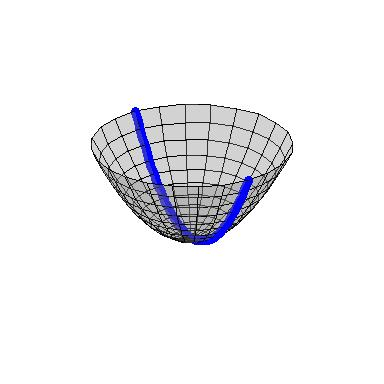
\includegraphics[width=2.5in]{./ParabolasGraphics/Paraboloid01.jpg} & 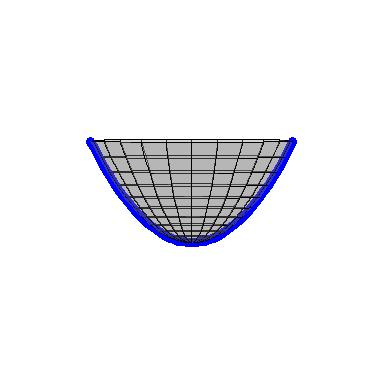
\includegraphics[width=2.5in]{./ParabolasGraphics/Paraboloid02.jpg} \\

\end{tabular}

\end{center}

Every cross section through the vertex of the paraboloid is a parabola with the same focus.  To see why this is important, imagine the dashed lines below as electromagnetic waves heading towards a parabolic dish.   It turns out that the waves reflect off the parabola and concentrate at the focus which then becomes the optimal place for the receiver. 

\smallskip

If, on the other hand, we imagine the dashed lines as emanating from the focus, we see that the waves are reflected off the parabola in a coherent fashion as in the case in a flashlight.  Here, the bulb is placed at the focus and the light rays are reflected off a parabolic mirror to give directional light.

\begin{center}

\begin{mfpic}[15]{-5}{7}{-1}{10}
\arrow \reverse \arrow \rotatepath{(0,0), -45}  \function{-6.25,6.25,0.1}{(x**2)/8}
\dashed  \rotatepath{(0,0), -45}   \polyline{(0,2), (2, 0.5), (2, 6)} 
\dashed  \rotatepath{(0,0), -45} \polyline{(0,2), (-2,0.5), (-2, 6)}
\dashed \rotatepath{(0,0), -45}   \polyline{(0,2), (4,2), (4, 6)}
\dashed \rotatepath{(0,0), -45}   \polyline{(0,2), (-4,2), (-4, 6)}
\dashed \rotatepath{(0,0), -45}  \polyline{(0,2), (6,4.5), (6, 6)}
\dashed \rotatepath{(0,0), -45}  \polyline{(0,2), (-6,4.5), (-6, 6)}
\plotsymbol[3pt]{Asterisk}{(1.414, 1.414)}
\tlabel[cc](2, 2){$F$}
\gfill \rotatepath{(0,0), -45}  \circle{(2,0.5),0.07}
\gfill \rotatepath{(0,0), -45}  \circle{(-2,0.5),0.07}
\gfill \rotatepath{(0,0), -45}  \circle{(4,2),0.07}
\gfill \rotatepath{(0,0), -45}  \circle{(-4,2),0.07}
\gfill \rotatepath{(0,0), -45} \circle{(6,4.5),0.07}
\gfill \rotatepath{(0,0), -45} \circle{(-6,4.5),0.07}
\end{mfpic}

\end{center}

\begin{ex} A satellite dish is to be constructed in the shape of a paraboloid of revolution.  If the receiver placed at the focus is located 2 ft above the vertex of the dish, and the dish is to be 12 feet wide, how deep will the dish be?

\smallskip

{\bf Solution.}  One way to approach this problem is to determine the equation of the parabola suggested to us by this data.  For simplicity, we'll assume the vertex is $(0,0)$ and the parabola opens upwards.  Our standard form for such a parabola is $x^2 = 4py$.  Since the focus is $2$ units above the vertex, we know  $p=2$, so we have $x^2 = 8y$.  Visually,

\begin{center}

\begin{mfpic}[25]{-7}{7}{0}{5}
\axes
\xmarks{-6, -5, -4, -3, -2, -1, 0,1,2,3,4,5,6}
\ymarks{0,1,2,3,4}
\arrow \polyline{(-5.5, 4.5),(5.5,4.5)}
\arrow \polyline{(5.5,4.5), (-5.5, 4.5)}
\arrow \polyline{(6, 0.5),(6,4)}
\arrow \polyline{(6,4), (6,0.5)}
\plotsymbol[3pt]{Asterisk}{(0, 2)}
\tlabel[cc](6.25,2.25){?}
\tlabel(6.25, 4.25){$(6,y)$}
\tlabel(0.25,5){$y$}
\tlabel(7, -0.25){$x$}
\gclear \tlabelrect[cc](0,4){$12$ units wide}
\tlpointsep{4pt}
\small
\axislabels {x}{{$-6 \hspace{7pt}$} -6, {$6$} 6}
\axislabels {y}{{$2$} 2}
\normalsize
\penwd{1.25pt}
\arrow \function{-6.25,6.25,0.1}{(x**2)/8}
\arrow \function{6.25,-6.25,0.1}{(x**2)/8}
\point[4pt]{(0,0), (6,36/8), (-6,36/8)}
\end{mfpic}

\end{center}

Since the parabola is $12$ feet wide, we know the edge is $6$ feet from the vertex.  To find the depth, we are looking for the $y$ value when $x=6$.  Substituting $x=6$ into the equation of the parabola yields $6^2 = 8y$ or $y = \frac{36}{8} = \frac{9}{2} = 4.5$.  Hence, the dish will be  $4.5$ feet deep.  \qed

\end{ex}

\newpage

\subsection{Exercises}

\label{ExercisesforParabolas}

In Exercises \ref{parabolasketchfirst} - \ref{parabolasketchlast},  graph of the given equations in the $xy$-plane.  Find the vertex, focus and directrix.  Include the endpoints of the latus rectum in your sketch.

\begin{multicols}{2}
\begin{enumerate}

\item $(x - 3)^{2} = -16y$ \label{parabolasketchfirst}
\item $\left(x + \frac{7}{3}\right)^{2} = 2\left(y + \frac{5}{2}\right)$


\setcounter{HW}{\value{enumi}}
\end{enumerate}
\end{multicols}

\begin{multicols}{2}
\begin{enumerate}
\setcounter{enumi}{\value{HW}}


\item \label{paranotfcnone} $(y - 2)^{2} = -12(x + 3)$ 
\item  \label{paranotfcntwo} $(y + 4)^{2} = 4x$

\setcounter{HW}{\value{enumi}}
\end{enumerate}
\end{multicols}

\begin{multicols}{2}
\begin{enumerate}
\setcounter{enumi}{\value{HW}}


\item $(x-1)^2 = 4(y+3)$
\item $(x+2)^2 = -20(y-5)$


\setcounter{HW}{\value{enumi}}
\end{enumerate}
\end{multicols}

\begin{multicols}{2}
\begin{enumerate}
\setcounter{enumi}{\value{HW}}

\item \label{paranotfcnthree} $(y-4)^2 = 18(x-2)$
\item  \label{paranotfcnfour} $\left(y+ \frac{3}{2}\right)^2 = -7 \left(x+ \frac{9}{2}\right)$ \label{parabolasketchlast}


\setcounter{HW}{\value{enumi}}
\end{enumerate}
\end{multicols}


In Exercises \ref{stdfrmparabolafirst} - \ref{stdfrmparabolalast}, put the equation into standard form.  Find the vertex, focus and directrix.\footnote{\ldots assuming the equation were graphed in the $xy$-plane.}

\begin{multicols}{2}
\begin{enumerate}
\setcounter{enumi}{\value{HW}}

\item  \label{paranotfcnfive} $y^{2} - 10y - 27x + 133 = 0$ \label{stdfrmparabolafirst}
\item $25x^{2} + 20x + 5y - 1 = 0$

\setcounter{HW}{\value{enumi}}
\end{enumerate}
\end{multicols}

\begin{multicols}{2}
\begin{enumerate}
\setcounter{enumi}{\value{HW}}

\item $x^2 + 2x - 8y + 49 = 0$
\item  \label{paranotfcnsix} $2y^2 + 4y +x - 8 = 0$

\setcounter{HW}{\value{enumi}}
\end{enumerate}
\end{multicols}

\begin{multicols}{2}
\begin{enumerate}
\setcounter{enumi}{\value{HW}}

\item $x^2-10x+12y+1=0$
\item   $3y^2-27y+4x+\frac{211}{4} = 0$ \label{stdfrmparabolalast}   \label{paranotfcnseven} 

\setcounter{HW}{\value{enumi}}
\end{enumerate}
\end{multicols}

\begin{enumerate}
\setcounter{enumi}{\value{HW}}


\item For each of the equations given in Exercises \ref{parabolasketchfirst} - \ref{stdfrmparabolalast} that do \textbf{not} describe $y$ as a function of $x$, find two or more explicit functions of $x$ represented by each of the equations.  (See Example \ref{horizontalparabolaex}.)


\setcounter{HW}{\value{enumi}}
\end{enumerate}

In Exercises \ref{buildparafromgraphfirst} - \ref{buildparafromgraphlast}, find an equation for the parabola whose graph is given.

\begin{multicols}{2}
\begin{enumerate}
\setcounter{enumi}{\value{HW}}

\item $~$ \label{buildparafromgraphfirst}

\begin{mfpic}[13]{-5}{5}{-5}{5}
\axes
\tlabel[cc](5,-0.5){\scriptsize $x$}
\tlabel[cc](0.5,5){\scriptsize $y$}
\tlabel[cc](1, 1){\scriptsize $(0,2)$}
\tlabel[cc](-2.25,-3.75){\scriptsize $(-2,-6)$}
\xmarks{-4,-3,-2,-1,1,2,3,4}
\ymarks{-4,-3,-2, -1, 1,2,3,4}
\tlpointsep{4pt}
\scriptsize
\axislabels {x}{ {$-4 \hspace{7pt}$} -4, {$-3 \hspace{7pt}$} -3, {$-2 \hspace{7pt}$} -2, {$-1 \hspace{7pt}$} -1, {$1$} 1, {$2$} 2, {$3$} 3, {$4$} 4}
\axislabels {y}{ 1, {$4$} 2, {$6$} 3, {$8$} 4, {$-4$} -2, {$-6$} -3}
\penwd{1.25pt}
\arrow \reverse \arrow \function{-4.8,0.8,0.1}{(x+2)**2-3}
\point[4pt]{(-2,-3), (0,1)}
\normalsize
\end{mfpic} 

\vfill

\columnbreak

\item $~$

\begin{mfpic}[13]{-5}{5}{-5}{5}
\axes
\tlabel[cc](5,-0.5){\scriptsize $x$}
\tlabel[cc](0.5,5){\scriptsize $y$}
\tlabel[cc](-1.25, 4.25){\scriptsize $(0,4)$}
\tlabel[cc](3,0.75){\scriptsize $(\sqrt{2},0)$}
\tlabel[cc](-3.25,0.75){\scriptsize $(-\sqrt{2},0)$}
\xmarks{-3,,-1,1,3}
\ymarks{-4,-3,-2, -1, 1,2,3,4}
\tlpointsep{4pt}
\scriptsize
\axislabels {x}{ {$-2 \hspace{7pt}$} -3, {$-1 \hspace{7pt}$} -1, {$1$} 1, {$2$} 3}
\axislabels {y}{{$-1$} -1,{$1$} 1, {$2$} 2, {$3$} 3,  {$-2$} -2, {$-3$} -3, {$-4$} -4}
\penwd{1.25pt}
\arrow \reverse \arrow \function{-3,3,0.1}{4-(x**2)}
\point[4pt]{(0,4), (-2,0), (2,0)}
\normalsize
\end{mfpic} 

\setcounter{HW}{\value{enumi}}
\end{enumerate}
\end{multicols}


\pagebreak

\begin{multicols}{2}
\begin{enumerate}
\setcounter{enumi}{\value{HW}}


\item $~$   

\begin{mfpic}[13]{-6}{5}{-3}{7}
\axes
\tlabel[cc](5,-0.5){\scriptsize $x$}
\tlabel[cc](0.5,7){\scriptsize $y$}
\tlabel[cc](-5.5, 2){\scriptsize $(-4,2)$}
\tlabel[cc](1, 4.75){\scriptsize $(0,4)$}
\tlabel[cc](1, -1){\scriptsize $(0, 0)$}
%\tlabel[cc](-0.5,-1){\scriptsize $\left(0, \frac{1}{2} \right)$}
\xmarks{-4,-3,-2,-1,1,2,3,4}
\ymarks{-2 step 1 until 6}
\tlpointsep{4pt}
\scriptsize
\axislabels {x}{ {$-4 \hspace{7pt}$} -4, {$-3 \hspace{7pt}$} -3, {$-2 \hspace{7pt}$} -2, {$-1 \hspace{7pt}$} -1,  {$4$} 4}
\axislabels {y}{{$1$} 1, {$2$} 2, {$3$} 3,  {$5$} 5,{$6$} 6, {$-1$} -1, {$-2$} -2}
\penwd{1.25pt}
\arrow  \function{-4,5,0.1}{2-sqrt(x+4)}
\arrow  \function{-4,5,0.1}{2+sqrt(x+4)}
\point[4pt]{(-4,2), (0,0), (0,4)}
%\tcaption{ \scriptsize $x$,$y$-intercept $(0,0)$}
\normalsize
\end{mfpic} 

\vfill

\columnbreak

\item $~$ \label{buildparafromgraphlast} 

\begin{mfpic}[13]{-5}{5}{-5}{5}
\axes
\tlabel[cc](5,-0.5){\scriptsize $x$}
\tlabel[cc](0.5,5){\scriptsize $y$}
\tlabel[cc](1.25,2){\scriptsize $(0,4)$}
\tlabel[cc](1.5,-2){\scriptsize $(0,-4)$}
\tlabel[cc](2,-0.75){\scriptsize $(1,0)$}
%\tlabel[cc](-1.5, 0.5){\scriptsize $(-1,0)$}
%\tlabel[cc](-0.5,-1){\scriptsize $\left(0, \frac{1}{2} \right)$}
\xmarks{-4,-3,-2,-1,1,2,3,4}
\ymarks{-4 step 1 until 4}
\tlpointsep{4pt}
\scriptsize
\axislabels {x}{ {$-4 \hspace{7pt}$} -4, {$-3 \hspace{7pt}$} -3, {$-2 \hspace{7pt}$} -2, {$-1 \hspace{7pt}$} -1,   {$4$} 4}
\axislabels {y}{{$2$} 1, {$4$} 2, {$6$} 3, {$8$} 4, {$-2$} -1, {$-4$} -2, {$-6$} -3, {$-8$} -4}
\penwd{1.25pt}
\arrow \reverse \function{-5,1,0.1}{2*sqrt(1-x)}
\arrow \reverse \function{-5,1,0.1}{-2*sqrt(1-x)}
\point[4pt]{(1,0), (0,2), (0,-2)}
%\tcaption{ \scriptsize $x$-intercept $(1,0)$, $y$-intercept $(0,2)$}
\normalsize
\end{mfpic} 


\setcounter{HW}{\value{enumi}}
\end{enumerate}
\end{multicols}


In Exercises \ref{buildparafirst} - \ref{buildparalast}, find an equation for the parabola which fits the given criteria.

\begin{multicols}{2}
\begin{enumerate}
\setcounter{enumi}{\value{HW}}

\item Vertex $(7, 0)$, focus $(0, 0)$. \label{buildparafirst}
\item Focus $(10, 1)$, directrix $x = 5$.


\setcounter{HW}{\value{enumi}}
\end{enumerate}
\end{multicols}

\begin{enumerate}
\setcounter{enumi}{\value{HW}}


\item Vertex $(-8, -9)$; $(0, 0)$ and $(-16, 0)$ are points on the curve.
\item The endpoints of latus rectum are $(-2, -7)$ and $(4, -7)$.\label{buildparalast}

\setcounter{HW}{\value{enumi}}
\end{enumerate}





\begin{enumerate}
\setcounter{enumi}{\value{HW}}

\item  The mirror in Carl's flashlight is a paraboloid of revolution.  If the mirror is 5 centimeters in diameter and 2.5 centimeters deep, where should the light bulb be placed so it is at the focus of the mirror?

\item  A parabolic Wi-Fi antenna is constructed by taking a flat sheet of metal and bending it into a parabolic shape.\footnote{This shape is called a `parabolic cylinder.'}  If the cross section of the antenna is a parabola which is 45 centimeters wide and 25 centimeters deep, where should the receiver be placed to maximize reception?

\item  \label{parabolaarch} A parabolic arch is constructed which is 6 feet wide at the base and 9 feet tall in the middle. Find the height of the arch exactly 1 foot in from the base of the arch. 

\item  A popular novelty item is the `mirage bowl.'  Follow this  \href{http://spie.org/etop/2007/etop07methodsV.pdf}{\underline{link}} to see another startling application of the reflective property of the parabola.

\item With the help of your classmates, research spinning liquid mirrors.  To get you started,  \href{http://www.astro.ubc.ca/LMT/lzt/}{\underline{here}}.

\end{enumerate}

\newpage

\subsection{Answers}

\begin{enumerate}

\item \begin{multicols}{2}
{\small $(x - 3)^{2} = -16y$}\\
{\small Vertex $(3, 0)$}\\
{\small Focus $(3, -4)$}\\
{\small Directrix $y = 4$}\\
{\small Endpoints of latus rectum $(-5, -4)$, $(11, -4)$}\\

\vfill

\columnbreak

\begin{mfpic}[10]{-6}{12}{-5}{5}
\axes
\xmarks{-5 step 1 until 11}
\ymarks{-4 step 1 until 4}
\arrow \reverse \arrow \polyline{(-6,4),(12,4)}
\plotsymbol[4pt]{Asterisk}{(3,-4)}
\tlabel(12,-0.5){\scriptsize $x$}
\tlabel(0.5,5){\scriptsize $y$}
\point[4pt]{(3,0),(-5,-4),(11,-4)}
\tlpointsep{4pt}
\tiny
\axislabels {x}{{$-5 \hspace{7pt}$} -5, {$-4 \hspace{7pt}$} -4, {$-3 \hspace{7pt}$} -3, {$-2 \hspace{7pt}$} -2, {$-1 \hspace{7pt}$} -1, {$1$} 1, {$2$} 2, {$3$} 3, {$4$} 4, {$5$} 5, {$6$} 6, {$7$} 7, {$8$} 8, {$9$} 9, {$10$} 10, {$11$} 11}
\axislabels {y}{{$-4$} -4, {$-3$} -3, {$-2$} -2, {$-1$} -1, {$1$} 1, {$2$} 2, {$3$} 3, {$4$} 4}
\normalsize
\penwd{1.25pt}
\arrow \reverse \arrow \function{-5.5,11.5,0.1}{((x - 3)**2)/(-16)}
\end{mfpic}
\end{multicols}

\smallskip

\item  \begin{multicols}{2}
{\small $\left(x + \frac{7}{3}\right)^{2} = 2\left(y + \frac{5}{2}\right)$}\\
{\small Vertex $\left(-\frac{7}{3}, -\frac{5}{2} \right)$}\\
{\small Focus $\left(-\frac{7}{3}, -2 \right)$}\\
{\small Directrix $y = -3$}\\
{\small Endpoints of latus rectum $\left(-\frac{10}{3}, -2 \right)$, $\left(-\frac{4}{3}, -2 \right)$}\\

\vfill

\columnbreak


\begin{mfpic}[15][20]{-6}{1}{-4}{3}
\axes
\xmarks{-5 step 1 until 0}
\ymarks{-3 step 1 until 2}
\arrow \reverse \arrow \polyline{(-5,-3),(1,-3)}
\plotsymbol[4pt]{Asterisk}{(-2.333,-2)}
\tlabel(1,-0.5){\scriptsize $x$}
\tlabel(0.5,3){\scriptsize $y$}
\point[4pt]{(-2.333,-2.5),(-3.333,-2),(-1.333,-2)}
\tlpointsep{4pt}
\tiny
\axislabels {x}{{$-5 \hspace{7pt}$} -5, {$-4 \hspace{7pt}$} -4, {$-3 \hspace{7pt}$} -3, {$-2 \hspace{7pt}$} -2, {$-1 \hspace{7pt}$} -1}
\axislabels {y}{{$-3$} -3, {$-2$} -2, {$-1$} -1, {$1$} 1, {$2$} 2}
\normalsize
\penwd{1.25pt}
\arrow \reverse \arrow \function{-5.5,0.8,0.1}{((x + (7/3))**2)/2 - (5/2)}
\end{mfpic}
\end{multicols}

\smallskip

\item \begin{multicols}{2} 

{\small $(y - 2)^{2} = -12(x + 3)$} \\
{\small Vertex $(-3, 2)$} \\
{\small Focus $(-6, 2)$} \\
{\small Directrix $x = 0$}\\
{\small Endpoints of latus rectum $(-6, 8)$, $(-6, -4)$}\\

\vfill

\columnbreak


\begin{mfpic}[10]{-8}{1}{-5}{9}
\axes
\xmarks{-7 step 1 until 0}
\ymarks{-4 step 1 until 8}
\plotsymbol[4pt]{Asterisk}{(-6,2)}
\tlabel(1,-0.5){\scriptsize $x$}
\tlabel(0.5,9){\scriptsize $y$}
\point[4pt]{(-3,2),(-6,-4),(-6,8)}
\tlpointsep{4pt}
\tiny
\axislabels {x}{{$-7 \hspace{7pt}$} -7, {$-6 \hspace{7pt}$} -6, {$-5 \hspace{7pt}$} -5, {$-4 \hspace{7pt}$} -4, {$-3 \hspace{7pt}$} -3, {$-2 \hspace{7pt}$} -2, {$-1 \hspace{7pt}$} -1}
\axislabels {y}{{$-4$} -4, {$-3$} -3, {$-2$} -2, {$-1$} -1, {$1$} 1, {$2$} 2, {$3$} 3, {$4$} 4, {$5$} 5, {$6$} 6, {$7$} 7, {$8$} 8}
\normalsize
\penwd{1.25pt}
\arrow \reverse \function{-6.8,-3,0.1}{2+sqrt((-12*x) - 36)}
\arrow \reverse \function{-6.8,-3,0.1}{2-sqrt((-12*x) - 36)}
\end{mfpic}
\end{multicols}

\pagebreak

\item \begin{multicols}{2} 
{\small $(y + 4)^{2} = 4x$}\\
{\small Vertex $(0,-4)$} \\
{\small Focus $(1,-4)$} \\
{\small Directrix $x = -1$}\\
{\small Endpoints of latus rectum $(1, -2)$, $(1, -6)$}\\

\vfill

\columnbreak


\begin{mfpic}[15]{-2}{5}{-9}{1}
\axes
\xmarks{-1 step 1 until 4}
\ymarks{-8 step 1 until 0}
\arrow \reverse \arrow \polyline{(-1,-9),(-1,1)}
\plotsymbol[4pt]{Asterisk}{(1,-4)}
\tlabel(5,-0.5){\scriptsize $x$}
\tlabel(0.5,1){\scriptsize $y$}
\point[4pt]{(0,-4),(1,-2),(1,-6)}
\tlpointsep{4pt}
\tiny
\axislabels {x}{{$-1 \hspace{7pt}$} -1, {$1$} 1, {$2$} 2, {$3$} 3, {$4$} 4}
\axislabels {y}{{$-8$} -8, {$-7$} -7, {$-6$} -6, {$-5$} -5, {$-4$} -4, {$-3$} -3, {$-2$} -2, {$-1$} -1}
\normalsize
\penwd{1.25pt}
\arrow \function{0,5,0.1}{-4-(2*sqrt(x))}
\arrow \function{0,5,0.1}{-4+(2*sqrt(x))}
\end{mfpic}
\end{multicols}

\smallskip


\item  \begin{multicols}{2}
{\small $(x-1)^2 = 4(y+3)$}\\
{\small Vertex $\left(1, -3\right)$}\\
{\small Focus $\left(1, -2 \right)$}\\
{\small Directrix $y = -4$}\\
{\small Endpoints of latus rectum $\left(3, -2 \right)$, $\left(-1, -2 \right)$}\\

\vfill

\columnbreak


\begin{mfpic}[15]{-4}{5}{-5}{1}
\axes
\xmarks{-3 step 1 until 4}
\ymarks{-4 step 1 until 0}
\arrow \reverse \arrow \polyline{(-5,-4),(5,-4)}
\plotsymbol[4pt]{Asterisk}{(1,-2)}
\tlabel(5,-0.5){\scriptsize $x$}
\tlabel(0.5,1){\scriptsize $y$}
\point[4pt]{(3,-2),(1,-3),(-1,-2)}
\tlpointsep{4pt}
\tiny
\axislabels {x}{{$-3 \hspace{7pt}$} -3, {$-2 \hspace{7pt}$} -2, {$-1 \hspace{7pt}$} -1, {$1$} 1, {$2$} 2, {$3$} 3, {$4$} 4}
\axislabels {y}{{$-4$} -4, {$-3$} -3, {$-2$} -2, {$-1$} -1}
\normalsize
\penwd{1.25pt}
\arrow \reverse \arrow \function{-3,5,0.1}{((x -1)**2)/4 - 3}
\end{mfpic}
\end{multicols}

\smallskip

\item \begin{multicols}{2}
{\small $(x+2)^2 = -20(y-5)$}\\
{\small Vertex $\left(-2, 5\right)$}\\
{\small Focus $\left(-2, 0 \right)$}\\
{\small Directrix $y = 10$}\\
{\small Endpoints of latus rectum $\left(-12, 0 \right)$, $\left(8, 0 \right)$}\\

\vfill

\columnbreak


\begin{mfpic}[7.5][10]{-13}{9}{-1}{11}
\axes
\xmarks{-12 step 1 until 8}
\ymarks{1 step 1 until 10}
\arrow \reverse \arrow \polyline{(-13,10),(9,10)}
\plotsymbol[4pt]{Asterisk}{(-2,0)}
\tlabel(9,-0.5){\scriptsize $x$}
\tlabel(0.5,11){\scriptsize $y$}
\point[4pt]{(-12,0),(-2,5),(8,0)}
\tlpointsep{4pt}
\tiny
\axislabels {x}{{$-12 \hspace{7pt}$} -12,  {$-10 \hspace{7pt}$} -10, {$-8 \hspace{7pt}$} -8, {$-6 \hspace{7pt}$} -6, {$-4 \hspace{7pt}$} -4,  {$-2 \hspace{7pt}$} -2, {$2$} 2,  {$4$} 4,  {$6$} 6, {$8$} 8}
\axislabels {y}{{$1$} 1, {$2$} 2, {$3$} 3, {$4$} 4, {$5$} 5, {$6$} 6, {$7$} 7, {$8$} 8, {$9$} 9, {$10$} 10}
\normalsize
\penwd{1.25pt}
\arrow \reverse \arrow \function{-13,9,0.1}{((x +2)**2)/(0-20) + 5}
\end{mfpic}
\end{multicols}

\smallskip


\item \begin{multicols}{2}
{\small $(y-4)^2 = 18(x-2)$}\\
{\small Vertex $\left(2, 4\right)$}\\
{\small Focus $\left( \frac{13}{2}, 4 \right)$}\\
{\small Directrix $x = -\frac{5}{2}$}\\
{\small Endpoints of latus rectum $\left(\frac{13}{2}, -5 \right)$, $\left(\frac{13}{2}, 13 \right)$}\\

\vfill

\columnbreak


\begin{mfpic}[15][7.5]{-3}{8}{-6}{14}
\axes
\xmarks{-2 step 1 until 7}
\ymarks{-5 step 1 until 13}
\arrow \reverse \arrow \polyline{(-2.5,-6),(-2.5,14)}
\plotsymbol[4pt]{Asterisk}{(6.5,4)}
\tlabel(8,-0.5){\scriptsize $x$}
\tlabel(0.5,14){\scriptsize $y$}
\point[4pt]{(6.5,-5),(2,4),(6.5,13)}
\tlpointsep{4pt}
\tiny
\axislabels {x}{{$-1$} -1, {$1$} 1,  {$2$} 2,  {$3$} 3, {$4$} 4, {$5$} 5,  {$6$} 6,  {$7$} 7}
\axislabels {y}{{$-5$} -5, {$-3$} -3, {$-1$} -1, {$1$} 1, {$3$} 3, {$5$} 5, {$7$} 7, {$9$} 9, {$11$} 11, {$13$} 13}
\normalsize
\penwd{1.25pt}
\arrow \function{2,8,0.1}{4+(sqrt(18*(x-2)))}
\arrow \function{2,8,0.1}{4-(sqrt(18*(x-2)))}
\end{mfpic}
\end{multicols}

\smallskip

\item \begin{multicols}{2} 
{\small $\left(y+ \frac{3}{2}\right)^2 = -7 \left(x+ \frac{9}{2}\right)$}\\
{\small Vertex $\left(-\frac{9}{2}, -\frac{3}{2}\right)$}\\
{\small Focus $\left( -\frac{25}{4}, -\frac{3}{2} \right)$}\\
{\small Directrix $x = -\frac{11}{4}$}\\
{\small Endpoints of latus rectum $\left(-\frac{25}{4}, 2 \right)$, $\left(-\frac{25}{4}, -5 \right)$}\\

\vfill

\columnbreak


\begin{mfpic}[15]{-7}{1}{-6}{3}
\axes
\xmarks{-6 step 1 until -1}
\ymarks{-5 step 1 until 2}
\arrow \reverse \arrow \polyline{(-2.75,-6),(-2.75,3)}
\plotsymbol[4pt]{Asterisk}{(-6.25,-1.5)}
\tlabel(1,-0.5){\scriptsize $x$}
\tlabel(0.5,3){\scriptsize $y$}
\point[4pt]{(-6.25,-5),(-4.5,-1.5),(-6.25,2)}
\tlpointsep{4pt}
\tiny
\axislabels {x}{{$-5 \hspace{7pt}$} -5,{$-4 \hspace{7pt}$} -4,{$-3 \hspace{7pt}$} -3,{$-2 \hspace{7pt}$} -2,{$-1 \hspace{7pt}$} -1}
\axislabels {y}{{$-5$} -5, {$-4$} -4, {$-3$} -3, {$-2$} -2, {$-1$} -1, {$1$} 1, {$2$} 2}
\normalsize
\penwd{1.25pt}
\arrow \function{-4.5,-7,0.1}{0-1.5+(sqrt((0-7)*(x+4.5)))}
\arrow \function{-4.5,-7,0.1}{0-1.5-(sqrt((0-7)*(x+4.5)))}
\end{mfpic}
\end{multicols}

\setcounter{HW}{\value{enumi}}
\end{enumerate}

\begin{multicols}{2}
\begin{enumerate}
\setcounter{enumi}{\value{HW}}


\item $(y - 5)^{2} = 27(x - 4)$\\
Vertex $(4, 5)$\\
Focus $\left( \frac{43}{4}, 5 \right)$\\
Directrix $x = -\frac{11}{4}$

\item $\left(x + \frac{2}{5} \right)^{2} = -\frac{1}{5}(y - 1)$\\
Vertex $\left( -\frac{2}{5}, 1 \right)$\\
Focus $\left( -\frac{2}{5}, \frac{19}{20} \right)$\\
Directrix $y = \frac{21}{20}$

\setcounter{HW}{\value{enumi}}
\end{enumerate}
\end{multicols}

\begin{multicols}{2}
\begin{enumerate}
\setcounter{enumi}{\value{HW}}


\item  $(x+1)^2=8(y-6)$ \\
Vertex $(-1,6)$\\
Focus $(-1,8)$ \\
Directrix $y=4$

\item  $(y+1)^2=-\frac{1}{2}(x-10)$\\
Vertex $(10,-1)$\\
Focus $\left(\frac{79}{8}, -1 \right)$\\
Directrix $x = \frac{81}{8}$

\setcounter{HW}{\value{enumi}}
\end{enumerate}
\end{multicols}

\begin{multicols}{2}
\begin{enumerate}
\setcounter{enumi}{\value{HW}}

\item $(x-5)^2 = -12(y-2)$\\
Vertex $(5,2)$\\
Focus $(5,-1)$ \\
Directrix $y=5$


\item  $\left(y-\frac{9}{2}\right)^2 = -\frac{4}{3} (x-2)$\\
Vertex $\left(2, \frac{9}{2}\right)$\\
Focus $\left(\frac{5}{3}, \frac{9}{2}\right)$\\
Directrix $x = \frac{7}{3}$

\setcounter{HW}{\value{enumi}}
\end{enumerate}
\end{multicols}

\begin{enumerate}
\setcounter{enumi}{\value{HW}}

\item  The equations which do not represent $y$ as a function of $x$ are:  \ref{paranotfcnone}, \ref{paranotfcntwo}, \ref{paranotfcnthree}, \ref{paranotfcnfour}, \ref{paranotfcnfive}, \ref{paranotfcnsix}, \ref{paranotfcnseven}.


For number \ref{paranotfcnone}:

\begin{itemize}

\item  $f(x) = 2+2 \sqrt{-3x-9}$ represents the upper half of the parabola.

\item  $g(x) =  2 - 2\sqrt{-3x-9}$ represents the lower half of the parabola.

\end{itemize}

For number \ref{paranotfcntwo}:

\begin{itemize}

\item  $f(x) = -4+2\sqrt{x}$ represents the upper half of the parabola.

\item  $g(x) =  -4 - 2\sqrt{x}$  represents the lower half of the parabola.

\end{itemize}


For number \ref{paranotfcnthree}:

\begin{itemize}

\item   $f(x) =4+3 \sqrt{2x-4}$ represents the upper half of the parabola.

\item  $g(x) =  4-3 \sqrt{2x-4}$  represents the lower half of the parabola.

\end{itemize}


For number \ref{paranotfcnfour}:

\begin{itemize}

\item   $f(x) =-\frac{3}{2} + \frac{1}{2} \sqrt{-28x - 126}$ represents the upper half of the parabola.

\item  $g(x) =-\frac{3}{2} -  \frac{1}{2} \sqrt{-28x - 126}$  represents the lower half of the parabola.

\end{itemize}


For number \ref{paranotfcnfive}:

\begin{itemize}

\item   $f(x) =5+3 \sqrt{3x-12}$ represents the upper half of the parabola.

\item  $g(x) =5- 3 \sqrt{3x-12}$ represents the lower half of the parabola.

\end{itemize}


For number \ref{paranotfcnsix}:

\begin{itemize}

\item   $f(x) =-1 + \frac{1}{2} \sqrt{-2x+20}$ represents the upper half of the parabola.

\item  $g(x) =-1 - \frac{1}{2} \sqrt{-2x+20}$ represents the lower half of the parabola.

\end{itemize}

For number \ref{paranotfcnseven}:

\begin{itemize}

\item   $f(x) = \frac{9}{2} + \frac{2}{3} \sqrt{-3x+6}$ represents the upper half of the parabola.

\item  $f(x) = \frac{9}{2} - \frac{2}{3} \sqrt{-3x+6}$ represents the lower half of the parabola.

\end{itemize}


\setcounter{HW}{\value{enumi}}
\end{enumerate}

\begin{multicols}{4}
\begin{enumerate}
\setcounter{enumi}{\value{HW}}

\item  $(x+2)^2 = \frac{1}{2} (y+6)$
\item  $x^2 = -\frac{1}{2}(y-4)$
\item $(y-2)^2=x+4$  \vphantom{$(x+2)^2 = \frac{1}{2} (y+6)$}
\item $y^2 = -16(x-1)$  \vphantom{$(x+2)^2 = \frac{1}{2} (y+6)$}


\setcounter{HW}{\value{enumi}}
\end{enumerate}
\end{multicols}


\begin{multicols}{3}
\begin{enumerate}
\setcounter{enumi}{\value{HW}}

\item $y^{2} = -28(x - 7)$
\item $(y - 1)^{2} = 10\left(x - \frac{15}{2} \right)$
\item $(x + 8)^{2} = \frac{64}{9}(y + 9)$

\setcounter{HW}{\value{enumi}}
\end{enumerate}
\end{multicols}

\begin{enumerate}
\setcounter{enumi}{\value{HW}}


\item $(x - 1)^{2} = 6\left(y + \frac{17}{2}\right)$ or $(x - 1)^{2} = -6\left(y + \frac{11}{2}\right)$

\setcounter{HW}{\value{enumi}}
\end{enumerate}





\begin{enumerate}
\setcounter{enumi}{\value{HW}}

\item  The bulb should be placed $0.625$ centimeters above the vertex of the mirror.\footnote{As verified by Carl himself!}

\item  The receiver should be placed $5.0625$ centimeters from the vertex of the cross section of the antenna.

\item  The arch can be modeled by $x^2=-(y-9)$ or $y=9-x^2$.  One foot in from the base of the arch corresponds to either $x = \pm 2$, so the height is $y=9-(\pm 2)^2=5$ feet.

\end{enumerate}

\closegraphsfile

\newpage

\section{Circles}

\mfpicnumber{1}

\opengraphsfile{Circles}

\setcounter{footnote}{0}

\setlength{\extrarowheight}{2pt}

\label{Circles}

Our next entry in the conic sections menagerie is the circle.  Recall from Geometry that a circle can be determined by fixing a point (called the center) and a positive number (called the radius) as follows. \index{circle ! radius of} \index{circle ! center of} \index{center ! of a circle} \index{radius ! of a circle}

\smallskip

\colorbox{ResultColor}{\bbm

\begin{defn} \label{circledefn}  A \textbf{circle} with center $(h,k)$ and radius $r>0$ is the set of all points $(x, y)$ in the plane whose distance to $(h,k)$ is $r$. \index{circle ! definition of} 

\end{defn} 

\ebm}

\smallskip

\begin{center}

\begin{mfpic}[15]{-5}{5}{-5}{5}
\arrow\reverse\arrow \polyline{(0.25,0.25), (2.55,2.55)}
\tlabel(-0.5,-0.8){$(h,k)$}
\tlabel(1,1.55){$r$}
\plotsymbol[3pt]{Cross}{(0,0)}
\point[3pt]{(2.8284,2.8284)}
\tlabel(3,3){$(x,y)$}
\penwd{1.25pt}
\circle{(0,0),4}
\end{mfpic}

\end{center}

From the diagram, we see that a point $(x,y)$ is on the circle if and only if its distance to $(h,k)$ is $r$.  We  express this relationship algebraically using the Distance Formula, Equation \ref{distanceformula}, as 

\[r = \sqrt{(x - h)^2 + (y-k)^2}\]  
By squaring both sides of this equation, we get an equivalent equation (since $r > 0$) which gives us the standard equation of a circle.

\smallskip

\colorbox{ResultColor}{\bbm

\begin{eqn}  \label{standardcircle} \index{circle ! standard equation} \textbf{The Standard Equation of a Circle:}  

The equation of a circle with center $(h,k)$ and radius $r >0$ is $(x-h)^2 + (y-k)^2 = r^2.$

\end{eqn}
  
\ebm}
  
\smallskip

Note in the standard equation of a circle, \textit{both} of the variables squared.  This is a quick way to distinguish the equation of a circle from that of a parabola in which only \textit{one} of the variables is squared.   

\smallskip

 We put Equation \ref{standardcircle} to good use in the following example.

\begin{ex} $~$

\begin{enumerate} 

\item \label{circleex1} For each of the equations below:

\begin{itemize}

\item  Graph the equation in the $xy$-plane.

\item  Find the center and radius.

\end{itemize}

\begin{multicols}{2}

\begin{enumerate}

\item $(x+2)^2+(y-1)^2 = 4$

\item  \label{ctscircleex} $3x^2 - 6x + 3y^2 + 4y -4 = 0$

\end{enumerate}

\end{multicols}

\item  Graph $f(x) = - \sqrt{4x-x^2}$.

\newpage

\item  Find the standard form of the circle satisfying the following characteristics:

\begin{enumerate}

\item  The points $(-1,3)$ and $(2,4)$ are the endpoints of a diameter.

\item  The circle whose graph is below.

\begin{center}

\begin{mfpic}[15]{-5}{1}{-1}{5}
\axes
\xmarks{-4, -3, -2, -1, 0}
\ymarks{1,2,3,4}
\tlabel(1,-0.5){\scriptsize $x$}
\tlabel(0.5,5){\scriptsize $y$}
\tlabel[cc](-2, -0.5){\scriptsize $(-2,0)$}
\tlabel[cc](1,2){\scriptsize $(0,2)$}
\tlpointsep{4pt}
\scriptsize
\axislabels {x}{ {$-4 \hspace{7pt}$} -4}
\axislabels {y}{ {$4$} 4}
\normalsize
\penwd{1.25pt}
\circle{(-2,2),2}
\point[4pt]{(-2,0), (0,2)}
\end{mfpic}

\end{center}

\end{enumerate}


\end{enumerate}

\smallskip

{\bf Solution.}  

\begin{enumerate}

\item   

\begin{enumerate}

\item Rewriting  $(x+2)^2+(y-1)^2 = 4$ as  $(x-(-2))^2+(y-1)^2 = (2)^2$, we identify $h = -2$, $k=1$ and $r = 2$.  Thus we have a circle centered at $(-2,1)$ with a radius of $2$.  

\smallskip

To help us create a detailed graph, we start from the center $(-2,1)$ and move  two units to the left and two units up and down to the right to identify four points on the graph.\footnote{Note the center of the circle is \textit{not} on the graph of the circle!} We get $(-2-2, 1) = (-4,1)$, $(-2+2, 1) = (0,1)$,  $(-2, 1+2) = (-2,3)$ and $(-2,1-2) = (-2,-1)$.  Our graph is below on the left.

\item In order to make use of Equation \ref{standardcircle}, we need to put $3x^2 - 6x + 3y^2 + 4y -4 = 0$ into standard form.  To that end, we complete the square on both the $x$ and $y$ terms and collect the constants to the other side of the equation as demonstrated below.


\[ \begin{array}{rclr} 3x^2 - 6x + 3y^2 + 4y -4 & = & 0 & \\ 
 3x^2 - 6x + 3y^2 + 4y & = & 4 & \text{add $4$ to both sides} \\ [3pt]
 3\left(x^2 - 2x \right) + 3\left(y^2 + \dfrac{4}{3} y\right) & = & 4 & \text{factor out leading coefficients} \\ [10pt]
 3\left(x^2 - 2x + \underline{1} \right) + 3\left(y^2 + \dfrac{4}{3} y + \underline{\underline{\dfrac{4}{9}}} \right) & = & 4 + 3\underline{(1)} + 3\underline{\underline{\left(\dfrac{4}{9}\right)}} &  \text{complete the square in $x$, $y$} \\  [10pt]
 3(x - 1)^2 + 3\left(y + \dfrac{2}{3}\right)^2 & = & \dfrac{25}{3} & \text{factor} \\ [10pt]
 (x - 1)^2 + \left(y + \dfrac{2}{3}\right)^2 & = & \dfrac{25}{9} & \text{divide both sides by $3$} \\ [10pt]
 (x - 1)^2 + \left(y - \left(- \dfrac{2}{3} \right) \right)^2 & = & \left( \dfrac{5}{3} \right)^2 & \text{rewrite in the form of Equation \ref{standardcircle}.}
 \end{array} \]
 

From Equation \ref{standardcircle}, we identify $h = 1$,  $k =  - \frac{2}{3}$, and $r   = \frac{5}{3}$.  Hence, we have a circle with center  $\left(1, -\frac{2}{3}\right)$ and radius  $ \frac{5}{3}$.  

\smallskip

As above, we find four points on the circle by starting at the center  $\left(1, -\frac{2}{3}\right)$ and moving up, down, to the left, and to the right $ \frac{5}{3}$ units.  Doing so produces the following points: $\left(-\frac{2}{3}, -\frac{2}{3}\right)$ , $\left(\frac{8}{3}, -\frac{2}{3}\right)$ ,   $\left(1, 1\right)$, and $\left(1, -\frac{7}{3}\right)$.  Our graph is below on the right.

\begin{center}

\begin{multicols}{2}

\begin{mfpic}[20]{-5}{2}{-2}{4}
\axes
\plotsymbol[3pt]{Cross}{(-2,1)}
\tlabel[cc](-2, 1.5){\scriptsize $(-2,1)$}
\tlabel[cc](1, 1){\scriptsize $(0,1)$}
\tlabel[cc](-5, 1){\scriptsize $(-4,1)$}
\tlabel[cc](-2, 3.5){\scriptsize $(-2,3)$}
\tlabel[cc](-2, -1.5){\scriptsize $(-2,-1)$}
\tcaption{\scriptsize The graph of $(x+2)^2+(y-1)^2 = 4$}
\xmarks{-4, -3, -2,-1,0, 1}
\ymarks{-1,0,1, 2,3}
\tlabel(2,-0.25){\scriptsize $x$}
\tlabel(0.25,4){\scriptsize $y$}
\tlpointsep{4pt}
\scriptsize
\axislabels {x}{{$-4 \hspace{7pt}$} -4, {$-3 \hspace{7pt}$} -3, {$-2 \hspace{7pt}$} -2, {$-1 \hspace{7pt}$} -1, {$1$} 1}
\axislabels {y}{{$-1$} -1, {$1$} 1,  {$3$} 3, {$4$} 4}
\normalsize
\penwd{1.25pt}
\circle{(-2,1),2}
\point[4pt]{(0,1), (-4,1), (-2,3), (-2,-1)}
\end{mfpic}

\begin{mfpic}[20]{-2}{5}{-4}{2}
\axes
\plotsymbol[3pt]{Cross}{(1, -0.6666)}
\tlabel[cc](-1.75, -0.6666){\scriptsize $\left(-\frac{2}{3}, -\frac{2}{3}\right)$}
\tlabel[cc](3.5, -0.6666){\scriptsize $\left(\frac{8}{3}, -\frac{2}{3}\right)$}
\tlabel[cc](1, 1.5){\scriptsize $\left(1, 1\right)$}
\tlabel[cc](1, -2.8){\scriptsize $\left(1, -\frac{7}{3}\right)$}
\tlabel[cc](1, -1.25){\scriptsize  $\left(1, -\frac{2}{3}\right)$}
\tcaption{\scriptsize The graph of $3x^2 - 6x + 3y^2 + 4y -4 = 0$}
\xmarks{-1, 1, 2, 3, 4}
\ymarks{-3,-2,-1,1}
\tlabel(5,-0.25){\scriptsize $x$}
\tlabel(0.25,2){\scriptsize $y$}
\tlpointsep{4pt}
\scriptsize
\axislabels {x}{ {$2$} 2}
\axislabels {y}{{$-3$} -3,  {$1$} 1}
\normalsize
\penwd{1.25pt}
\circle{(1,-0.6666),1.6666}
\point[4pt]{(-0.6666,-0.6666), (2.6666,-0.6666), (1,1), (1,-2.3333)}
\end{mfpic}

\end{multicols}

\end{center}

\end{enumerate}

\item  We are asked to graph $f(x) = - \sqrt{4x-x^2}$, which, at first glance, seems out of place in this section. However, to graph means we graph the equation  $y = -\sqrt{4x-x^2}$.  

\smallskip

Squaring both sides, we get  $y^2 = (-\sqrt{4x-x^2})^2$ or   $y^2 = 4x - x^2$.  Rearranging this equation gives $x^2-4x+y^2 = 0$.   Completing the square, we obtain $(x-2)^2 + y^2  = 4$ which, when rewritten as $(x-2)^2 + (y-0)^2 = (2)^2$ is precisely the standard form of a circle as written in Equation \ref{standardcircle}.  


\smallskip

With $h = 2$, $k=0$ and $r=2$, we know the graph of   $(x-2)^2 + y^2  = 4$ is a circle of radius $2$ centered at $(2,0)$.  However,  the graph we want isn't the \textit{entire} circle.\footnote{For one thing, the graph of a circle fails the Vertical Line Test so it does not represent $y$ as a function of $x$ in this case.}  Indeed, we want the graph of $y = -\sqrt{4x-x^2}$. Because of the `$-$ ',  we want the \textit{lower} semicircle, graphed below on the left.

\item 

\begin{enumerate}

\item  We recall that a diameter of a circle is a line segment containing the center and two points on the circle.  We plot the data given to us below on the right.

\begin{center}

\begin{multicols}{2}

\begin{mfpic}[20]{-2}{5}{-3}{3}
\axes
\plotsymbol[3pt]{Cross}{(2,0) }
\tlabel[cc](2, -2.5){\scriptsize $(2,-2)$}
\tlabel[cc](0.5, 0.25){\scriptsize $(0,0)$}
\tlabel[cc](3.5, 0.25){\scriptsize $(4,0)$}
\tlabel[cc](2, 0.25){\scriptsize $(2,0)$}
\dotted \circle{(2,0),2}
\tcaption{\scriptsize The graph of $f(x) = - \sqrt{4x-x^2}$.}
\xmarks{-1, 1,  3, 4}
\ymarks{-2,-1,1,2}
\tlabel(5,-0.25){\scriptsize $x$}
\tlabel(0.25,3){\scriptsize $y$}
\tlpointsep{4pt}
\scriptsize
\axislabels {x}{ {$1$} 1,  {$2$} 2, {$3$} 3}
\axislabels {y}{{$-2$} -2,  {$-1$} -1,  {$1$} 1,  {$2$} 2}
\normalsize
\penwd{1.25pt}
\plrfcn{90,180,5}{4*cosd(t)}
\point[4pt]{(0,0), (2,-2), (4,0)}
\end{mfpic}



\begin{mfpic}[20]{-2}{4}{-0.5}{5.5}
\axes
\dashed \circle{(0.5,3.5),3.162277660/2}
\point[4pt]{(-1,3), (2,4)}
\plotsymbol[3pt]{Cross}{(0.5,3.5)}
\xmarks{-2,-1,0,1,2,3}
\ymarks{0,1,2,3,4,5}
\tlabel(4,-0.25){ \scriptsize $x$}
\tlabel(0.25,5.5){ \scriptsize $y$}
\arrow \reverse \arrow \polyline{(0.75,3.583),(1.75,3.916)}
\tlabel[cc](0.85,3){\scriptsize $(h,k)$}
\tlabel[cc](1.15,4){\scriptsize $r$}
\tlpointsep{4pt}
\scriptsize
\axislabels {x}{{$-2 \hspace{7pt}$} -2, {$-1 \hspace{7pt}$} -1, {$1$} 1, {$2$} 2, {$3$} 3}
\axislabels {y}{{$1$} 1, {$2$} 2, {$3$} 3, {$4$} 4, {$5$}, 5}
\normalsize

\end{mfpic}


\end{multicols}
\end{center}

Since the given points are endpoints of a diameter, we know their midpoint $(h, k)$ is the center of the circle.  Likewise, the diameter of the circle is the distance between the given points, so we can find the radius of the circle by taking half of this distance.  Using Equations \ref{midpointformula} and \ref{distanceformula}, respectively, we get:

\begin{multicols}{2}

$\begin{array}{rcl} (h,k) &  = & \left( \dfrac{x_{\text{\tiny$0$}} + x_{\text{\tiny$1$}}}{2},  \dfrac{y_{\text{\tiny$0$}} + y_{\text{\tiny$1$}}}{2} \right) \\ [8pt]
&  = &  \left( \dfrac{-1+2}{2},  \dfrac{3+4}{2} \right) \\ [8pt]
& = &  \left( \dfrac{1}{2},  \dfrac{7}{2} \right)   \\  [8pt]
&& \\ \end{array}$

$\begin{array}{rcl} r &  = & \dfrac{1}{2} \sqrt{\left(x_{\text{\tiny$1$}} - x_{\text{\tiny$0$}}\right)^2+\left(y_{\text{\tiny$1$}}-y_{\text{\tiny$0$}}\right)^2}  \\ [8pt]
 &  = & \dfrac{1}{2} \sqrt{(2-(-1))^2+(4-3)^2} \\ [8pt]
 & = & \dfrac{1}{2} \sqrt{3^2+1^2} \\ [8pt]
 & = &\dfrac{\sqrt{10}}{2} \end{array} $
 
 \end{multicols}
 
 
Finally, since $\left( \frac{\sqrt{10}}{2} \right)^2 = \frac{10}{4} = \frac{5}{2}$, our answer becomes $\left(x - \frac{1}{2} \right)^2 + \left(y - \frac{7}{2} \right)^2 =\frac{5}{2}$

\item  From the graph given to us, we are safe to assume the center of the circle is $(-2,2)$ since the circle appears to be \textit{tangent} to the coordinate axes at $(-2,0)$ and $(0,2)$.\footnote{Recall that for every point $P$ on the circle, the tangent line at $P$ is perpendicular to the radial line containing the center and $P$. Since the circle is tangent to the $x$-axis at $(-2,0)$, the center must lie on a line perpendicular to the $x$-axis which contains $(-2,0)$ or $x = -2$.  Likewise,  the circle is tangent to the $y$-axis at $(0,2)$,  the center must lie on $y=2$.  Hence the center is $(-2,2)$.}   Moreover, since the distance from $(-2,2)$ to either of $(-2,0)$ or $(0,2)$ is $2$, the radius of the circle is $2$.  Per Equation \ref{standardcircle}, our answer is $(x-(-2))^2 + (y-2)^2 = (2)^2$ or $(x+2)^2+(y-2)^2 = 4$. \qed

\end{enumerate}

\end{enumerate}

\end{ex}

In number \ref{ctscircleex} above, we needed to transform a given equation into the standard form as stated in Equation \ref{standardcircle}.  We record these steps below.  Note that given an equation that represents a circle, \textit{both} variables need to be squared and the squared terms must have the \textit{same} coefficients.

\smallskip

\colorbox{ResultColor}{\bbm

\centerline{\textbf{To Write the Equation of a Circle in Standard Form}}

\begin{enumerate}

\item  Group common variables together on one side of the equation and put the constant on the other.

\item  Complete the square on both variables as needed.

\item  Divide both sides by the coefficient of the squares. (For circles, they will be the same.)

\end{enumerate}

\ebm}

\smallskip

It is possible to obtain equations like $(x-3)^2 + (y+1)^2 = 0$ or $(x-3)^2 + (y+1)^2 = -1$, neither of which describes a circle. (Do you see why not?)  The reader is encouraged to think about what, if any, points lie on the graphs of these two equations.  

\smallskip

We close this section with a brief discussion of the so-called  \textit{Unit Circle}.\footnote{Widely regarded as the most important circle in all of mathematics.}

\bigskip

\colorbox{ResultColor}{\bbm

\begin{defn}

The \textbf{Unit Circle} \index{Unit Circle ! definition of} \label{UnitCircle} is the circle centered at $(0,0)$ with a radius of $1$.  The standard equation of the Unit Circle is $x^2 + y^2 = 1.$

\end{defn}

\ebm}

\smallskip

In some ways, we may think of the Unit Circle as the progenitor of all circles.  Indeed, if we divide both sides of Equation \ref{standardcircle} by $r^2$, we obtain the alternate standard form of a circle below.  

\smallskip

\colorbox{ResultColor}{\bbm

\begin{eqn} \label{standardcirclealternate} \index{circle ! standard equation, alternate} \textbf{The Alternate Standard Equation of a Circle:}  The equation of a circle with center $(h,k)$ and radius $r >0$ is

\[ \dfrac{(x-h)^2}{r^2} + \dfrac{(y-k)^2}{r^2} = 1 \]

\end{eqn}

\ebm}

\smallskip

Taking this one step further, we may rewrite Equation \ref{standardcirclealternate} as  \[ \left( \dfrac{x-h}{r} \right)^2 +  \left( \dfrac{y-k}{r} \right)^2 = 1. \] Hence, every circle can be obtained from the Unit Circle via the transformations discussed in Section \ref{Transformations}.\footnote{See Exercise \ref{circletransunitcircleexercise}.}

\smallskip

Our last example has us find some important points on the the Unit Circle.

\smallskip

\begin{ex}  Find the points on the unit circle with $y$-coordinate $\frac{\sqrt{3}}{2}$.

\medskip

{\bf Solution.}  Note that all points $(x,y)$ on the Unit Circle satisfy the equation $x^2+y^2 = 1$. Hence, our first step is  to replace $y$ with $\frac{\sqrt{3}}{2}$ and solve for $x$. 

 \[ \begin{array}{rclr} x^2 + y^2 & = & 1 & \\
 x^2 + \left(\dfrac{\sqrt{3}}{2}\right)^2 & = & 1 &  \\ [13pt]
 \dfrac{3}{4} + x^2 & = & 1 & \\
 x^2 & = & \dfrac{1}{4} & \\
 x  & = & \pm \sqrt{\dfrac{1}{4}} & \text{extract square roots} \\ [7pt]
 x & = & \pm \dfrac{1}{2} & \\  \end{array} \]


We find $x = \pm \frac{1}{2}$ so our final answers are  $\left(\frac{1}{2}, \frac{\sqrt{3}}{2} \right)$ and $\left(-\frac{1}{2}, \frac{\sqrt{3}}{2} \right)$.  \qed

\end{ex}

\newpage

\subsection{Exercises}

\label{ExercisesforCircles}

In Exercises \ref{circleeqnfirst} - \ref{circleeqnlast}, graph the circle in the $xy$-plane.  Find the center and radius.

\begin{multicols}{2}
\begin{enumerate}

\item $(x + 1)^{2} + (y + 5)^{2} = 100$ \label{circleeqnfirst} \label{oddcircleone}
\item $(x-4)^2+(y+2)^2 = 9$

\setcounter{HW}{\value{enumi}}
\end{enumerate}
\end{multicols}

\begin{multicols}{2}
\begin{enumerate}
\setcounter{enumi}{\value{HW}}

\item $\left(x + 3\right)^{2} + \left(y - \frac{7}{13}\right)^{2} = \frac{1}{4}$ \label{oddcirclethree}

\item $(x - 5)^{2} + (y + 9)^{2} = (\ln(8))^{2}$


\setcounter{HW}{\value{enumi}}
\end{enumerate}
\end{multicols}

\begin{multicols}{2}
\begin{enumerate}
\setcounter{enumi}{\value{HW}}


\item $(x  + e)^{2} + \left(y - \sqrt{2} \right)^{2} = \pi^{2}$  \label{oddcirclefive}

\item $\left(x - \pi \right)^{2} + \left(y -  e^{2}\right)^{2} = 91^{\frac{2}{3}}$ \label{circleeqnlast}

\setcounter{HW}{\value{enumi}}
\end{enumerate}
\end{multicols}


In Exercises \ref{ctscirclefirst} - \ref{ctscirclelast}, complete the square in order to put the equation into standard form.  Identify the center and the radius or explain why the equation does not represent a circle.\footnote{\ldots assuming the equation were graphed in the $xy$-plane.}


\begin{multicols}{2}
\begin{enumerate}
\setcounter{enumi}{\value{HW}}

\item $x^{2} - 4x + y^{2} + 10y = -25$  \label{ctscirclefirst}  \label{oddcircleseven}
\item $-2x^{2} - 36x - 2y^{2} - 112 = 0$

\setcounter{HW}{\value{enumi}}
\end{enumerate}
\end{multicols}

\begin{multicols}{2}
\begin{enumerate}
\setcounter{enumi}{\value{HW}}


\item $3x^2+3y^2+24x-30y -3 =0$  \label{oddcirclenine}
\item $x^2+y^2+5x-y-1=0$

\setcounter{HW}{\value{enumi}}
\end{enumerate}
\end{multicols}

\begin{multicols}{2}
\begin{enumerate}
\setcounter{enumi}{\value{HW}}


\item $x^{2} + x + y^{2} - \frac{6}{5}y = 1$  \label{oddcircleeleven}
\item $4x^{2} + 4y^{2} - 24y + 36 = 0$ \label{ctscirclelast}

\setcounter{HW}{\value{enumi}}
\end{enumerate}
\end{multicols}

\begin{enumerate}
\setcounter{enumi}{\value{HW}}

\item For each of the odd numbered equations given in Exercises \ref{oddcircleone} - \ref{oddcircleeleven}, find two or more explicit functions of $x$ represented by each of the equations.  (See Example \ref{horizontalparabolaex} in Section \ref{Parabolas}.)

\setcounter{HW}{\value{enumi}}
\end{enumerate}


In Exercises \ref{semicirclefunctionfirst} - \ref{semicirclefunctionlast}, graph each function by recognizing it as a semicircle.

\begin{multicols}{2}
\begin{enumerate}
\setcounter{enumi}{\value{HW}}

\item   $f(x) = \sqrt{4-x^2}$ \label{semicirclefunctionfirst}
\item   $g(x) = -\sqrt{6x-x^2}$

\setcounter{HW}{\value{enumi}}
\end{enumerate}
\end{multicols}

\begin{multicols}{2}
\begin{enumerate}
\setcounter{enumi}{\value{HW}}

\item  $f(x) = -\sqrt{3-2x-x^2}$
\item  $g(x) = -2 + \sqrt{9-x^2}$ \label{semicirclefunctionlast}

\setcounter{HW}{\value{enumi}}
\end{enumerate}
\end{multicols}

In Exercises \ref{buildcirclefromgraphfirst} - \ref{buildcirclefromgraphlast}, find an equation for the circle or semicircle whose graph is given.

\begin{multicols}{2}
\begin{enumerate}
\setcounter{enumi}{\value{HW}}

\item $~$ \label{buildcirclefromgraphfirst}

\begin{mfpic}[13]{-4}{6}{-5}{5}
\axes
\tlabel[cc](6,-0.5){\scriptsize $x$}
\tlabel[cc](0.5,5){\scriptsize $y$}
\tlabel[cc](1, 3.5){\scriptsize $(1,3)$}
\tlabel[cc](1.25, -3.75){\scriptsize $(1,-3)$}
\tlabel[cc](-3, 0.75){\scriptsize $(-2,0)$}
\tlabel[cc](5, 0.75){\scriptsize $(4,0)$}
\xmarks{-3 step 1 until 5}
\ymarks{-4 step 1 until 4}
\tlpointsep{4pt}
\scriptsize
\axislabels {x}{ {$-3 \hspace{7pt}$} -3,  {$-1 \hspace{7pt}$} -1, {$1$} 1, {$2$} 2, {$3$} 3, {$5$} 5}
\axislabels {y}{ {$-4$} -4, {$-2$} -2, {$-1$} -1, {$1$} 1, {$2$} 2,  {$4$} 4  }
\penwd{1.25pt}
\circle{(1,0), 3}
\point[4pt]{(-2,0), (4,0), (1,3), (1,-3)}
\normalsize
\end{mfpic} 

\vfill

\columnbreak

\item $~$

\begin{mfpic}[13]{-1}{9}{-1}{9}
\axes
\tlabel[cc](9,-0.5){\scriptsize $x$}
\tlabel[cc](0.5,9){\scriptsize $y$}
\tlabel[cc](1, 4){\scriptsize $(0,4)$}
\tlabel[cc](7, 4){\scriptsize $(8,4)$}
\tlabel[cc](4, 8.75){\scriptsize $(4,8)$}
\tlabel[cc](4, 0.75){\scriptsize $(4,0)$}
\xmarks{1 step 1 until 8}
\ymarks{1 step 1 until 8}
\tlpointsep{4pt}
\scriptsize
\axislabels {x}{{$1$} 1, {$2$} 2, {$3$} 3, {$4$} 4, {$5$} 5, {$6$} 6, {$7$} 7, {$8$} 8}
\axislabels {y}{{$1$} 1, {$2$} 2, {$3$} 3, {$4$} 4, {$5$} 5, {$6$} 6, {$7$} 7, {$8$} 8}
\penwd{1.25pt}
\circle{(4,4), 4}
\point[4pt]{(4,0), (0,4), (4,8), (8,4)}
\normalsize
\end{mfpic} 

\setcounter{HW}{\value{enumi}}
\end{enumerate}
\end{multicols}



\begin{multicols}{2}
\begin{enumerate}
\setcounter{enumi}{\value{HW}}


\item $~$   

\begin{mfpic}[13]{-5}{5}{-1}{6}
\axes
\tlabel[cc](5,-0.5){\scriptsize $x$}
\tlabel[cc](0.5,6){\scriptsize $y$}
\tlabel[cc](-4, 4.5){\scriptsize $(-4,4)$}
\tlabel[cc](4, 4.5){\scriptsize $(4,4)$}
\tlabel[cc](0.75, -0.75){\scriptsize $(0, 0)$}
%\tlabel[cc](-0.5,-1){\scriptsize $\left(0, \frac{1}{2} \right)$}
\xmarks{-4,-3,-2,-1,1,2,3,4}
\ymarks{1 step 1 until 5}
\tlpointsep{4pt}
\scriptsize
\axislabels {x}{ {$-4 \hspace{7pt}$} -4, {$-3 \hspace{7pt}$} -3, {$-2 \hspace{7pt}$} -2, {$-1 \hspace{7pt}$} -1,  {$4$} 4,  {$3$} 3,  {$2$} 2}
\axislabels {y}{{$1$} 1, {$2$} 2, {$3$} 3,  {$4$} 4,  {$5$} 5}
\penwd{1.25pt}
\function{-4,4,0.1}{4-sqrt(16-(x**2))}
\point[4pt]{(-4,4), (0,0), (4,4)}
%\tcaption{ \scriptsize $x$,$y$-intercept $(0,0)$}
\normalsize
\end{mfpic} 

\vfill

\columnbreak

\item $~$ \label{buildcirclefromgraphlast} 

\begin{mfpic}[13]{-1}{9}{-1}{6}
\axes
\tlabel[cc](9,-0.5){\scriptsize $x$}
\tlabel[cc](0.5,6){\scriptsize $y$}
\tlabel[cc](8, -0.75){\scriptsize $(8,0)$}
\tlabel[cc](4, 4.5){\scriptsize $(4,4)$}
\tlabel[cc](-0.75, -0.75){\scriptsize $(0, 0)$}
%\tlabel[cc](-0.5,-1){\scriptsize $\left(0, \frac{1}{2} \right)$}
\xmarks{1 step 1 until 8}
\ymarks{1 step 1 until 5}
\tlpointsep{4pt}
\scriptsize
\axislabels {x}{{$1$} 1,  {$2$} 2,  {$3$} 3,  {$4$} 4,  {$5$} 5,  {$6$} 6, {$7$} 7 }
\axislabels {y}{{$1$} 1, {$2$} 2, {$3$} 3,  {$4$} 4,  {$5$} 5}
\penwd{1.25pt}
\function{0,8,0.1}{sqrt(8*x-(x**2))}
\point[4pt]{(8,0), (0,0), (4,4)}
%\tcaption{ \scriptsize $x$,$y$-intercept $(0,0)$}
\normalsize
\end{mfpic} 


\setcounter{HW}{\value{enumi}}
\end{enumerate}
\end{multicols}


In Exercises \ref{buildcirclefirst} - \ref{buildcirclelast}, find the standard equation of the circle which satisfies the given criteria.

\begin{multicols}{2}
\begin{enumerate}
\setcounter{enumi}{\value{HW}}

\item center $(3, 5)$,  passes through $(-1, -2)$ \label{buildcirclefirst}

\item  center $(3, 6)$,  passes through  $(-1, 4)$

\setcounter{HW}{\value{enumi}}
\end{enumerate}
\end{multicols}

\begin{multicols}{2}
\begin{enumerate}
\setcounter{enumi}{\value{HW}}

\item  endpoints of a diameter: $(3,6)$ and $(-1,4)$

\item endpoints of a diameter:  $\left( \frac{1}{2}, 4\right)$, $\left(\frac{3}{2}, -1\right)$  \label{buildcirclelast}

\setcounter{HW}{\value{enumi}}
\end{enumerate}
\end{multicols}


\begin{enumerate}
\setcounter{enumi}{\value{HW}}

\item The Giant Wheel at Cedar Point is a circle with diameter 128 feet which sits on an 8 foot tall platform making its overall height is 136 feet.\footnote{Source: \href{http://www.cedarpoint.com/public/park/rides/tranquil/giant_wheel.cfm}{\underline{Cedar Point's webpage}}.}  Find an equation for the wheel assuming that its center lies on the $y$-axis and that the ground is the $x$-axis.
\label{giantwheelcircle}

\item Verify that the following points lie on the Unit Circle:

 $(\pm 1, 0)$, $(0, \pm 1)$, $\left(\pm \frac{\sqrt{2}}{2}, \pm \frac{\sqrt{2}}{2}\right)$, $\left(\pm \frac{1}{2}, \pm \frac{\sqrt{3}}{2}\right)$ and  $\left(\pm \frac{\sqrt{3}}{2}, \pm \frac{1}{2}\right)$


\item \label{circletransunitcircleexercise} Discuss with your classmates how to obtain the alternate standard equation of a circle, Equation \ref{standardcirclealternate}, from the equation of the Unit Circle, $x^2+y^2=1$ using the transformations discussed in Section \ref{Transformations}.  (Thus every circle is just a few transformations away from the Unit Circle.)

\item Find a one-to-one function whose graph is half of a circle. 

HINT:  Think piecewise \ldots

\end{enumerate}

\newpage

\subsection{Answers}

\begin{multicols}{2}
\begin{enumerate}


\item Center $(-1, -5)$, radius $10$ \\

\begin{mfpic}[6]{-12}{10}{-16}{6}
\axes
\plotsymbol[4pt]{Cross}{(-1,-5)}
\xmarks{-11,-1,9}
\ymarks{-15,-5,5}
\tlabel(10,-0.5){\scriptsize $x$}
\tlabel(0.5,6){\scriptsize $y$}
\tlabel(0.5,-5.25){\tiny $-5$}
\tlpointsep{4pt}
\tiny
\axislabels {x}{{$-11 \hspace{6pt}$} -11, {$-1 \hspace{6pt}$} -1, {$9$} 9}
\axislabels {y}{{$-15$} -15, {$5$} 5}
\normalsize
\penwd{1.25pt}
\circle{(-1,-5),10}
\end{mfpic}

\vfill

\columnbreak

\item  Center $(4,-2)$, radius $3$ \\
 
\begin{mfpic}[15.5]{-1}{8}{-6}{2}
\axes
\plotsymbol[4pt]{Cross}{(4,-2)}
\xmarks{1,4,7}
\ymarks{-5,-2,1}
\tlabel(8,-0.5){\scriptsize $x$}
\tlabel(0.5,2){\scriptsize $y$}
\tlpointsep{4pt}
\tiny
\axislabels {x}{{$1$} 1,{$4$} 4,{$7$} 7}
\axislabels {y}{{$-5$} -5, {$-2$} -2, {$1$} 1 }
\normalsize
\penwd{1.25pt}
\circle{(4,-2),3}
\end{mfpic}

\setcounter{HW}{\value{enumi}}
\end{enumerate}
\end{multicols}

\begin{multicols}{2}
\begin{enumerate}
\setcounter{enumi}{\value{HW}}

\item Center $\left(-3, \frac{7}{13}\right)$, radius $\frac{1}{2}$ \\

\begin{mfpic}[35]{-4}{1}{-0.75}{2}
\axes
\plotsymbol[4pt]{Cross}{(-3,0.53846)}
\xmarks{-3.5,-3,-2.5}
\ymarks{0.03846, 0.53836, 1.03846}
\tlabel(1,-0.25){\scriptsize $x$}
\tlabel(0.25,2){\scriptsize $y$}
\tlpointsep{4pt}
\tiny
\axislabels {x}{{$-\frac{7}{2} \hspace{6pt}$} -3.5, {$-3 \hspace{6pt}$} -3, {$-\frac{5}{2} \hspace{6pt}$} -2.5}
\axislabels {y}{{$\frac{1}{26}$} 0.03846, {$\frac{7}{13}$} 0.53846, {$\frac{27}{26}$} 1.03846}
\normalsize
\penwd{1.25pt}
\circle{(-3,0.53846),0.5}
\end{mfpic}

\vfill

\columnbreak

\item Center $(5, -9)$, radius $\ln(8)$ \\

\begin{mfpic}[10]{-1}{8}{-12}{1}
\axes
\plotsymbol[4pt]{Cross}{(5,-9)}
\xmarks{2.92055, 5, 7.07944}
\ymarks{-11.07944, -9, -6.92055}
\tlabel(8,0.5){\scriptsize $x$}
\tlabel(0.5,1){\scriptsize $y$}
\tlpointsep{4pt}
\tiny
\axislabels {x}{{$5 - \ln(8)$} 2.92055, {$5$} 5, {$5 + \ln(8)$} 7.07944}
\axislabels {y}{{$-9 - \ln(8)$} -11.07944, {$-9$} -9, {$-9 + \ln(8)$} -6.92055}
\normalsize
\penwd{1.25pt}
\circle{(5, -9),2.0794}
\end{mfpic}

\setcounter{HW}{\value{enumi}}
\end{enumerate}
\end{multicols}

\begin{multicols}{2}
\begin{enumerate}
\setcounter{enumi}{\value{HW}}

\item Center $\left(-e, \sqrt{2}\right)$, radius $\pi$ \\
 

\begin{mfpic}[10]{-7}{3}{-3}{6}
\axes
\plotsymbol[4pt]{Cross}{(-2.71828, 1.41421)}
\xmarks{-5.85987, -2.71828, 0.42331}
\ymarks{-1.72738,1.41421, 4.55581}
\tlabel(3,0.5){\scriptsize $x$}
\tlabel(0.5,6){\scriptsize $y$}
\tlpointsep{4pt}
\tiny
\axislabels {x}{{$-e-\pi$} -6.85987, {$-e$} -2.71828, {$-e+\pi$} 1.42331}
\tlabel(0.5,-2.22738){$\sqrt{2}-\pi$}
\tlabel(0.5,1.41421){$\sqrt{2}$}
\tlabel(0.5,4.55581){$\sqrt{2}+\pi$}
\normalsize
\penwd{1.25pt}
\circle{(-2.71828, 1.41421),3.14159}
\end{mfpic}

\vfill

\columnbreak

\item Center $(\pi, e^{2})$, radius $\sqrt[3]{91}$ \\

\begin{mfpic}[10]{-2}{8.25}{-0.25}{13}
\axes
\plotsymbol[4pt]{Cross}{(3.14159,7.389)}
\xmarks{-1.3563, 3.14159, 7.6395}
\ymarks{2.8911, 7.389, 11.88699}
\tlabel(8.25,0.5){\scriptsize $x$}
\tlabel(0.25,13){\scriptsize $y$}
\tlpointsep{4pt}
\tiny
\axislabels {x}{{$\pi - \sqrt[3]{91}$} -1.3563, {$\pi$} 3.14159, {$\pi + \sqrt[3]{91}$} 7.6395}
\axislabels {y}{{$e^{2} - \sqrt[3]{91}$} 2.8911, {$e^{2}$} 7.389, {$e^{2} + \sqrt[3]{91}$} 11.88699}
\normalsize
\penwd{1.25pt}
\circle{(3.14159,7.389),4.4979}
\end{mfpic}

\setcounter{HW}{\value{enumi}}
\end{enumerate}
\end{multicols}

\begin{multicols}{2}
\begin{enumerate}
\setcounter{enumi}{\value{HW}}

\item $(x - 2)^{2} + (y + 5)^{2} = 4$\\
Center $(2, -5)$, radius $r = 2$

\item $(x + 9)^{2} + y^{2} = 25$\\
Center $(-9, 0)$, radius $r = 5$

\setcounter{HW}{\value{enumi}}
\end{enumerate}
\end{multicols}

\begin{multicols}{2}
\begin{enumerate}
\setcounter{enumi}{\value{HW}}

\item $(x+4)^2 + (y-5)^2 = 42$ \\
Center $(-4,5)$, radius $r = \sqrt{42}$

\item $\left(x + \frac{5}{2}\right)^2 + \left(y - \frac{1}{2}\right)^2 = \frac{30}{4}$ \\
Center $\left( -\frac{5}{2}, \frac{1}{2}\right)$, radius $r = \frac{\sqrt{30}}{2}$

\setcounter{HW}{\value{enumi}}
\end{enumerate}
\end{multicols}

\begin{multicols}{2}
\begin{enumerate}
\setcounter{enumi}{\value{HW}}

\item $\left(x + \frac{1}{2}\right)^{2} + \left(y - \frac{3}{5}\right)^{2} = \frac{161}{100}$\\
Center $\left(-\frac{1}{2}, \frac{3}{5}\right)$, radius $r = \frac{\sqrt{161}}{10}$

\item $x^{2} + (y - 3)^{2} = 0$\\
This is not a circle.

\setcounter{HW}{\value{enumi}}
\end{enumerate}
\end{multicols}

\begin{enumerate}
\setcounter{enumi}{\value{HW}}

\item $~$


For number \ref{oddcircleone}:

\begin{itemize}

\item  $f(x) = -5 + \sqrt{99-2x-x^2}$ represents the upper semicircle.

\item  $g(x) = -5 - \sqrt{99-2x-x^2}$ represents the lower semicircle.

\end{itemize}

For number \ref{oddcirclethree}:

\begin{itemize}

\item  $f(x) = \frac{7}{13} + \frac{1}{2} \sqrt{-4x^2-24x-35}$ represents the upper semicircle.

\item  $g(x) = \frac{7}{13} - \frac{1}{2} \sqrt{-4x^2-24x-35}$ represents the lower semicircle.

\end{itemize}

For number \ref{oddcirclefive}:

\begin{itemize}

\item  $f(x) = \sqrt{2} + \sqrt{\pi^2-e^2-2ex-x^2}$ represents the upper semicircle.

\item  $g(x) = \sqrt{2} - \sqrt{\pi^2-e^2-2ex-x^2}$  represents the lower semicircle.

\end{itemize}


For number \ref{oddcircleseven}:

\begin{itemize}

\item  $f(x) = -5 + \sqrt{4x-x^2}$ represents the upper semicircle.

\item  $g(x) =  -5 - \sqrt{4x-x^2}$   represents the lower semicircle.

\end{itemize}

For number \ref{oddcirclenine}:

\begin{itemize}

\item  $f(x) = 5 + \sqrt{26-8x-x^2}$ represents the upper semicircle.

\item  $g(x) =  5 - \sqrt{26-8x-x^2}$   represents the lower semicircle.

\end{itemize}

For number \ref{oddcircleeleven}:

\begin{itemize}

\item  $f(x) = \frac{3}{5} + \frac{1}{5} \sqrt{34-25x-25x^2}$ represents the upper semicircle.

\item  $g(x) =  \frac{3}{5} - \frac{1}{5} \sqrt{34-25x-25x^2}$   represents the lower semicircle.

\end{itemize}


\setcounter{HW}{\value{enumi}}
\end{enumerate}

\begin{multicols}{2}
\begin{enumerate}
\setcounter{enumi}{\value{HW}}

\item $f(x) = \sqrt{4-x^2}$

\begin{mfpic}[15]{-5}{5}{-1}{5}
\axes
\tlabel[cc](5,-0.5){\scriptsize $x$}
\tlabel[cc](0.5,5){\scriptsize $y$}
\tlabel[cc](-4, -0.5){\scriptsize $(-2,0)$}
\tlabel[cc](4, -0.5){\scriptsize $(2, 0)$}
\tlabel[cc](-1, 4.5){\scriptsize $(0,2)$}
\xmarks{-4 step 2 until 4}
\ymarks{0 step 2 until 4}
\tlpointsep{4pt}
\scriptsize
\axislabels {x}{ {$-1 \hspace{7pt}$} -2,  {$1$} 2}
\axislabels {y}{ {$1$} 2 }
\penwd{1.25pt}
\function{-4,4,0.1}{sqrt(16-(x**2))}
\point[4pt]{(-4,0), (0,4), (4,0)}
\normalsize
\end{mfpic} 

\vfill

\columnbreak

\item $g(x) = -\sqrt{6x-x^2}$

\begin{mfpic}[15]{-1}{7}{-4.5}{1.5}
\axes
\tlabel[cc](7,-0.5){\scriptsize $x$}
\tlabel[cc](0.5,1.5){\scriptsize $y$}
\tlabel[cc](3, -3.5){\scriptsize $(3,-3)$}
\tlabel[cc](-0.75, 0.75){\scriptsize $(0,0)$}
\tlabel[cc](6, 0.75){\scriptsize $(6,0)$}
\xmarks{1 step 1 until 6}
\ymarks{-4 step 1 until -1}
\tlpointsep{4pt}
\scriptsize
\axislabels {x}{{$1$} 1, {$2$} 2, {$3$} 3, {$4$} 4, {$5$} 5}
\axislabels {y}{{$-1$} -1, {$-2$} -2, {$-3$} -3, {$-4$} -4}
\penwd{1.25pt}
\function{0, 6, 0.1}{-sqrt(6*x-(x**2))}
\point[4pt]{(0,0), (3,-3), (6,0)}
\normalsize
\end{mfpic} 

\setcounter{HW}{\value{enumi}}
\end{enumerate}
\end{multicols}



\begin{multicols}{2}
\begin{enumerate}
\setcounter{enumi}{\value{HW}}

\item  $f(x) = -\sqrt{3-2x-x^2}$

\begin{mfpic}[20]{-4}{4}{-4}{4}
\axes
\tlabel[cc](4,-0.5){\scriptsize $x$}
\tlabel[cc](0.5,4){\scriptsize $y$}
\tlabel[cc](-3, 0.5){\scriptsize $(-3,0)$}
\tlabel[cc](-1.25, -2.5){\scriptsize $(-1,-2)$}
\tlabel[cc](1, 0.5){\scriptsize $(1,0)$}
\xmarks{-3 step 1 until 3}
\ymarks{-3 step 1 until 3}
\tlpointsep{4pt}
\scriptsize
\axislabels {x}{ {$-1 \hspace{7pt}$} -1, {$-2 \hspace{7pt}$} -2, {$2$} 2,{$3$} 3}
\axislabels {y}{ {$1$} 1, {$2$} 2,{$3$} 3,  {$-1$} -1}
\penwd{1.25pt}
\function{-3,1,0.1}{-sqrt(3-2*x-(x**2))}
\point[4pt]{(-3,0), (-1,-2), (1,0)}
\normalsize
\end{mfpic} 



\item  $g(x) = -2 + \sqrt{9-x^2}$

\begin{mfpic}[20]{-4}{4}{-4}{4}
\axes
\tlabel[cc](4,-0.5){\scriptsize $x$}
\tlabel[cc](0.5,4){\scriptsize $y$}
\tlabel[cc](1,1.25){\scriptsize $(0,1)$}
\tlabel[cc](-3, -2.5){\scriptsize $(-3,-2)$}
\tlabel[cc](3, -2.5){\scriptsize $(3,-2)$}
\xmarks{-3 step 1 until 3}
\ymarks{-3 step 1 until 3}
\tlpointsep{4pt}
\scriptsize
\axislabels {x}{ {$-1 \hspace{7pt}$} -1, {$-2 \hspace{7pt}$} -2, {$-3 \hspace{7pt}$} -3, {$2$} 2, {$3$} 3, {$1$} 1}
\axislabels {y}{ {$2$} 2,{$3$} 3, {$-1$} -1, {$-2$} -2, {$-3$} -3}
\penwd{1.25pt}
\function{-3,3,0.1}{-2+sqrt(9-(x**2))}
\point[4pt]{(0,1), (-3,-2), (3,-2)}
\normalsize
\end{mfpic} 

\setcounter{HW}{\value{enumi}}
\end{enumerate}
\end{multicols}


\begin{multicols}{2}
\begin{enumerate}
\setcounter{enumi}{\value{HW}}

\item  $(x-1)^2+y^2=9$

\item  $(x-4)^2+(y-4)^2=16$

\setcounter{HW}{\value{enumi}}
\end{enumerate}
\end{multicols}

\begin{multicols}{2}
\begin{enumerate}
\setcounter{enumi}{\value{HW}}

\item  $y = 4-\sqrt{16-x^2}$

\item $y = \sqrt{8x-x^2}$

\setcounter{HW}{\value{enumi}}
\end{enumerate}
\end{multicols}




\begin{multicols}{2}
\begin{enumerate}
\setcounter{enumi}{\value{HW}}

\item $(x - 3)^{2} + (y - 5)^{2} = 65$

\item  $(x-3)^2+(y-6)^2 = 20$

\setcounter{HW}{\value{enumi}}
\end{enumerate}
\end{multicols}

\begin{multicols}{2}
\begin{enumerate}
\setcounter{enumi}{\value{HW}}

\item  $(x-1)^2 + (y-5)^2 = 5$

\item $(x-1)^2 + \left(y - \frac{3}{2}\right)^2 = \frac{13}{2}$

\setcounter{HW}{\value{enumi}}
\end{enumerate}
\end{multicols}

\begin{enumerate}
\setcounter{enumi}{\value{HW}}

\item $x^{2} + (y - 72)^{2} = 4096$

\end{enumerate}

\closegraphsfile

\newpage

\section{Ellipses}

\mfpicnumber{1}

\opengraphsfile{Ellipses}

\setcounter{footnote}{0}

\label{Ellipses}

In the definition of a circle, Definition \ref{circledefn}, we fixed a point called the \textbf{center} and considered all of the points which were a fixed distance $r$ from that one point.  For our next conic section, the ellipse, we fix two distinct points and a distance $d$ to use in our definition.  

\smallskip

\colorbox{ResultColor}{\bbm

 \begin{defn} \label{ellipsedefn} Given two distinct points $F_{\mbox{\tiny$1$}}$ and $F_{\mbox{\tiny$2$}}$ in the plane and a fixed distance $d$, an \index{ellipse ! definition of}  \textbf{ellipse} is the set of all points $(x, y)$ in the plane such that the sum of each of the distances from $F_{\mbox{\tiny$1$}}$ and $F_{\mbox{\tiny$2$}}$ to $(x, y)$ is $d$.  The points $F_{\mbox{\tiny$1$}}$ and $F_{\mbox{\tiny$2$}}$ are called the \index{ellipse ! foci} \index{focus (foci) ! of an ellipse} \textbf{foci}\footnote{the plural of `focus'} of the ellipse.

\end{defn} 

\ebm}

\smallskip

\begin{center}

\begin{mfpic}[20]{-6}{6}{-5}{5}

\dashed \polyline{(-3,0), (4,2.4)}
\dashed \polyline{(3,0), (4,2.4)}

\tlabel[cc](5, 2.4){$(x, y)$}
\tlabel[cc](-1,1.1){$d_{\mbox{\tiny$1$}}$}
\tlabel[cc](3,1.1){$d_{\mbox{\tiny$2$}}$}
\tlabel[cc](-3,-0.5){$F_{\mbox{\tiny$1$}}$}
\tlabel[cc](3,-0.5){$F_{\mbox{\tiny$2$}}$}
\plotsymbol[3pt]{Asterisk}{(-3,0)}
\plotsymbol[3pt]{Asterisk}{(3,0)}
\tcaption{$d_{\mbox{\tiny$1$}} + d_{\mbox{\tiny$2$}} = d$ for all $(x, y)$ on the ellipse}
\penwd{1.25pt}
\ellipse{(0,0),5,4}
\point[4pt]{(4,2.4)}
\end{mfpic}

\end{center}


We may imagine taking a length of string and anchoring it to two points on a piece of paper.  The curve traced out by taking a pencil and moving it so the string is always taut is an ellipse.  Each ellipse has an assortment of parameters associated with it which we sketch below.

 
\begin{center}

\begin{mfpic}[20]{-6}{6}{-5}{5}
\dotted[1pt, 3pt] \polyline{(-5,0), (5,0)}
\dotted[1pt, 3pt] \polyline{(0,-4), (0,4)}
\tlabel[cc](-3,-0.5){$F_{\mbox{\tiny$1$}}$}
\tlabel[cc](3,-0.5){$F_{\mbox{\tiny$2$}}$}
\plotsymbol[3pt]{Asterisk}{(-3,0),(3,0)}
\plotsymbol[3pt]{Cross}{(0,0)}
\tlabel[cc](5.5,0){$V_{\mbox{\tiny$2$}}$}
\tlabel[cc](-5.5,0){$V_{\mbox{\tiny$1$}}$}
\gclear \tlabelrect[cc](0,-0.5){$C$}
\tlabel[cc](2.5,0.5){\tiny Major Axis}
\tlabel[cc](-0.5,2){\tiny \rotatebox{90}{Minor Axis}}
\penwd{1.25pt}
\ellipse{(0,0),5,4}
\point[4pt]{(5,0),(-5,0)}
\end{mfpic}

An ellipse with center $C$; foci $F_{\mbox{\tiny$1$}}$, $F_{\mbox{\tiny$2$}}$; and vertices $V_{\mbox{\tiny$1$}}$, $V_{\mbox{\tiny$2$}}$

\end{center} 

As depicted above,  the \index{ellipse ! center}\index{center ! of an ellipse}\textbf{center} of the ellipse is the midpoint of the line segment connecting the two foci.  The \index{ellipse ! major axis}\index{major axis of an ellipse}\textbf{major axis} of the ellipse is the line segment connecting two opposite ends of the ellipse which also contains the center and foci.  The \index{ellipse ! minor axis}\index{minor axis of an ellipse}\textbf{minor axis} of the ellipse is the line segment connecting two opposite ends of the ellipse which contains the center but is perpendicular to the major axis.  The \index{ellipse ! vertices}\index{vertex ! of an ellipse}\textbf{vertices} of an ellipse are the points of the ellipse which lie on the major axis. 

\smallskip

 Notice that the center is also the midpoint of the major axis, hence it is the midpoint of the vertices. Also note that the major axis is the longer of the two axes through the center, hence the moniker `major.'  Likewise, the minor axis is the shorter of the two, whence the adjective `minor.' 


\smallskip

In order to derive the standard equation of an ellipse, we assume that the ellipse has its center at $(0,0)$, its major axis along the $x$-axis, and has foci $(c,0)$ and $(-c,0)$ and vertices $(-a,0)$ and $(a,0)$.  We will label the $y$-intercepts of the ellipse as $(0,b)$ and $(0,-b)$  (We assume $a$, $b$, and $c$ are all positive numbers.) 

\smallskip

\begin{center}

\begin{mfpic}[20]{-6}{6}{-5}{5}
\axes
\dashed \polyline{(-3,0), (4,2.4)}
\dashed \polyline{(3,0), (4,2.4)}
\tlabel[cc](-3,-0.5){$(-c,0)$}
\tlabel[cc](3,-0.5){$(c,0)$}
\plotsymbol[3pt]{Asterisk}{(-3,0),(3,0)}
\plotsymbol[3pt]{Cross}{(0,0)}
\tlabel[cc](-6,-0.5){$(-a,0)$}
\tlabel[cc](6,-0.5){$(a,0)$}
\tlabel[cc](1,4.5){$(0,b)$}
\tlabel[cc](1, -4.5){$(0,-b)$}
\tlabel[cc](5, 2.4){$(x,y)$}
\tlabel(6,0.25){\scriptsize $x$}
\tlabel(-0.5,5){\scriptsize $y$}
\penwd{1.25pt}
\ellipse{(0,0),5,4}
\point[4pt]{(4,2.4),(-5,0),(5,0),(0,4),(0,-4)}
\end{mfpic}

\end{center}

\smallskip

Note that since $(a,0)$ is on the ellipse, it must satisfy the conditions of Definition \ref{ellipsedefn}.  That is, the distance from $(-c,0)$ to $(a,0)$ plus the distance from  $(c,0)$ to $(a,0)$ must equal the fixed distance $d$.  Since all of these points lie on the $x$-axis, we get

\[ \begin{array}{rclr} \mbox{distance from $(-c,0)$ to $(a,0)$} + \mbox{distance from $(c,0)$ to $(a,0)$} & = & d & \\ (a+c) + (a-c) & = & d & \\ 2a & = & d \\ \end{array}\]

\smallskip

In other words, the fixed distance $d$ mentioned in the definition of the ellipse is none other than the length of the major axis.  We now use that fact $(0,b)$ is on the ellipse, along with the fact that $d=2a$ to get

\[ \begin{array}{rclr} \mbox{distance from  $(-c,0)$ to $(0,b)$} + \mbox{distance from $(c,0)$ to $(0,b)$} & = & 2a & \\ \sqrt{(0-(-c))^2+(b-0)^2} + \sqrt{(0-c)^2+(b-0)^2} & = & 2a & \\ \sqrt{b^2+c^2}+\sqrt{b^2+c^2} & = & 2a  \\ 2 \sqrt{b^2+c^2} & = & 2a \\ \sqrt{b^2+c^2} & = & a \end{array}\]

\smallskip

From this, we get $a^2 = b^2 + c^2$, or $b^2 = a^2 - c^2$, which will prove useful later.  Now consider a point $(x,y)$ on the ellipse.  Applying Definition \ref{ellipsedefn}, we get


\[ \begin{array}{rclr} \mbox{distance from  $(-c,0)$ to $(x,y)$} + \mbox{distance from $(c,0)$ to $(x,y)$} & = & 2a & \\ \sqrt{(x-(-c))^2+(y-0)^2} + \sqrt{(x-c)^2+(y-0)^2} & = & 2a & \\ \sqrt{(x+c)^2+y^2}+\sqrt{(x-c)^2+y^2} & = & 2a  \\ \end{array}\]

\smallskip

In order to make sense of this situation, we need to make good use of Intermediate Algebra.

\[ \begin{array}{rclr}  \sqrt{(x+c)^2+y^2}+\sqrt{(x-c)^2+y^2} & = & 2a  & \\ \sqrt{(x+c)^2+y^2} & = & 2a - \sqrt{(x-c)^2+y^2} & \\ \left(\sqrt{(x+c)^2+y^2}\right)^2 & = & \left(2a - \sqrt{(x-c)^2+y^2}\right)^2 & \\ (x+c)^2+y^2 & = & 4a^2 - 4a\sqrt{(x-c)^2+y^2} + (x-c)^2+y^2 & \\ 4a\sqrt{(x-c)^2+y^2} & = & 4a^2 + (x-c)^2 - (x+c)^2 & \\ 4a\sqrt{(x-c)^2+y^2} & = & 4a^2 - 4cx & \\ a\sqrt{(x-c)^2+y^2} & = & a^2 - cx & \\ \left(a\sqrt{(x-c)^2+y^2}\right)^2 & = & \left(a^2 - cx\right)^2 & \\ a^2\left((x-c)^2+y^2\right) & = & a^4 - 2a^2cx +c^2 x^2 & \\  a^2x^2 - 2a^2cx + a^2c^2+a^2 y^2 & = & a^4 - 2a^2cx +c^2 x^2 & \\  a^2x^2 - c^2 x^2 +a^2 y^2 & = & a^4  - a^2c^2 & \\ \left(a^2 - c^2\right) x^2 +a^2 y^2 & = & a^2 \left(a^2 - c^2\right)  & \\ \end{array}\]

\smallskip

We are nearly finished.  Recall that $b^2 = a^2 - c^2$ so that

\[ \begin{array}{rclr} \left(a^2 - c^2\right)x^2 +a^2 y^2 & = & a^2\left(a^2 - c^2\right) & \\ b^2 x^2 +a^2 y^2 & = & a^2 b^2 & \\  \dfrac{x^2}{a^2} + \dfrac{y^2}{b^2} & = & 1 &  \\ \end{array}\]

\smallskip

This equation is for an ellipse centered at the origin. To get the formula for the ellipse centered at $(h,k)$, we could use the transformations from Section \ref{Transformations} or re-derive the equation using Definition \ref{ellipsedefn} and the distance formula to obtain the formula below.

\smallskip

\colorbox{ResultColor}{\bbm

\begin{eqn}  \label{standardellipse} \index{ellipse ! standard equation} \textbf{The Standard Equation of an Ellipse:}  

For positive unequal numbers $a$ and $b$, the equation of an ellipse with center $(h,k)$ is

\[ \dfrac{(x-h)^2}{a^2} + \dfrac{(y-k)^2}{b^2} = 1 \]

\end{eqn}
  
\ebm}
  
\smallskip

Some remarks about Equation \ref{standardellipse} are in order.  First note that the values $a$ and $b$ determine how far in the $x$ and $y$ directions, respectively, one counts from the center to arrive at points on the ellipse.  

\smallskip

Also  note that if $a > b$, then we have an ellipse whose major axis is horizontal, and hence, the foci lie to the left and right of the center.  In this case, as we've seen in the derivation, the distance from the center to the focus, $c$, can be found by $c = \sqrt{a^2 - b^2}$. 

\smallskip

If $b > a$, the roles of the major and minor axes are reversed, and the foci lie above and below the center. In this case, $c = \sqrt{b^2 - a^2}$.  In either case, it's best to just remember that $c$ is the distance from the center to each focus, and, formulaically,  $c = \sqrt{\mbox{bigger denominator} - \mbox{smaller denominator}}$.  

\smallskip

Finally, it is worth mentioning that if we compare Equation \ref{standardellipse} with the alternate standard equation of the circle, Equation \ref{standardcirclealternate}, the only difference between the forms is that with a circle, the denominators are the same, and with an ellipse, they are different.  

\smallskip

If we take a transformational approach, we can consider both Equations \ref{standardellipse} and \ref{standardcirclealternate} as shifts and stretches of the Unit Circle $x^2 + y^2 = 1$ in Definition \ref{UnitCircle}.  Replacing $x$ with $(x-h)$ and $y$ with $(y-k)$ causes the usual horizontal and vertical shifts.  Replacing $x$ with $\frac{x}{a}$ and $y$ with $\frac{y}{b}$ causes the usual vertical and horizontal stretches. 

\smallskip

 In other words, it is perfectly fine to think of an ellipse as the deformation of a circle in which the circle is stretched farther in one direction than the other.


\smallskip

\begin{ex} \label{ellipsesfirstex} $~$

\begin{enumerate}

\item  Graph each of the following equations below in the $xy$-plane.  Find the center, the lines which contain the major and minor axes, the vertices, the endpoints of the minor axis, and the foci.

\begin{enumerate}

\item  $25(x+1)^2 + 9(y-2)^2 = 225$.  

\item \label{ctsellipseex}  $x^2+4y^2-2x+24y+33 = 0$.

\end{enumerate}

\item  Graph $f(x) = 1 + 2\sqrt{-x^2-4x-3}$

\item  Find the standard form of the equation of an ellipse which satisfies the following characteristics:

\begin{enumerate}

\item  the foci are at $(2,1)$ and $(4,1)$ and vertex $(0,1)$.

\newpage

\item  the ellipse graphed below:

\begin{center}

\begin{mfpic}[20]{-1}{7}{-5}{5}
\axes
\tlabel[cc](7,-0.5){\scriptsize $x$}
\tlabel[cc](0.5,5){\scriptsize $y$}
\tlabel[cc](0.5,0.3){\scriptsize $(0,0)$}
\tlabel[cc](1.5,2.75){\scriptsize $(1,3)$}
\tlabel[cc](5.3,0.3){\scriptsize $(6,0)$}
\xmarks{1,2,3,4,5,6}
\ymarks{-4, -3, -2, -1, 0, 1, 2, 3, 4}
\tlpointsep{4pt}
\scriptsize
\axislabels {x}{   {$1$} 1,  {$2$} 2,  {$3$} 3,  {$4$} 4,  {$5$} 5}
\axislabels {y}{{$-4$} -4,{$-3$} -3,  {$-2$} -2, {$-1$} -1, {$1$} 1, {$2$} 2, {$3$} 3, {$4$} 4}
\normalsize
\penwd{1.25pt}
\ellipse{(3,0),3,4.025}
\point[4pt]{(0,0), (6,0), (1,3)}
\end{mfpic}

\end{center}


\end{enumerate}


\end{enumerate}

\smallskip

{\bf Solution.} 

\begin{enumerate}

\item 

\begin{enumerate}

\item To put   $25(x+1)^2 + 9 (y-2)^2 = 225$ in the form prescribed by Equation \ref{standardellipse}, we rewrite the quantity $(x+1)$ as $(x-(-1))$ and divide through by $225$ to obtain an expression equal to $1$:  

\[  25 (x+1)^2 + 9 (y-2)^2 = 225 \rightarrow \dfrac{(x-(-1))^2}{9}  + \dfrac{(y-2)^2}{25} = 1 \leftrightarrow  \dfrac{(x-(-1))^2}{(3)^2}  + \dfrac{(y-2)^2}{(5)^2} = 1.  \]

We identify $h = -1$ and  $k = 2$, so the center of the ellipse is $(-1,2)$.  We have $a = 3$ so  we move $3$ units left and right from the center to obtain two points on the ellipse:  $(-1-3, 2) = (-4,2)$ and $(-1+3, 2) = (2,2)$.  Likewise, since $b=5$, we move up and down $5$ units from the center to find two more points on the ellipse: $(-1,2+5) = (-1,7)$ and $(-1, 2-5) = (-1,-3)$.

\smallskip

As an aid to sketching, we draw a rectangle matching this description, called a \index{ellipse ! guide rectangle}\index{guide rectangle ! for an ellipse}\textbf{guide rectangle}, and sketch the ellipse inside this rectangle as seen below on the left.

\smallskip

Since we moved farther from the center in the $y$ direction than in the $x$ direction, the major axis will lie along the vertical line $x=-1$, while the minor axis lies along the horizontal line $y = 2$.  The vertices are the points on the ellipse which lie along the major axis so in this case, they are the points $(-1,7)$ and $(-1,-3)$, and the endpoints of the minor axis are $(-4,2)$ and $(2,2)$.  (Notice these points are the four points we used to draw the guide rectangle.)  

\smallskip

To find the foci, we find $c = \sqrt{25-9} = \sqrt{16} = 4$, which means the foci lie $4$ units from the center. Since the major axis is vertical, the foci lie $4$ units above and below the center, at $(-1, 2-4) = (-1,-2)$ and $(-1, 2+4) = (-1,6)$.  Our final graph appears below on the right.

\begin{center}

\begin{tabular}{cc}

\begin{mfpic}[20]{-5}{3}{-4}{8}
\axes
\tlabel(3,-0.5){\scriptsize $x$}
\tlabel(0.5,8){\scriptsize $y$}
\tlabel[cc](-4.75,2){\scriptsize $(-4,2)$}
\tlabel[cc](2.5,2){\scriptsize $(2,2)$}
\tlabel[cc](-1,7.5){\scriptsize $(-1,7)$}
\tlabel[cc](-1,-3.5){\scriptsize $(-1,-3)$}
\tcaption{\scriptsize The graph of $25(x+1)^2 + 9 (y-2)^2 = 225$.}
\xmarks{-4, -3, -2, -1, 0, 1, 2}
\ymarks{-3, -2, -1, 0, 1, 2, 3, 4, 5, 6, 7}

\dotted[1pt, 3pt] \polyline{(-4,-3), (2,-3), (2,7), (-4,7), (-4,-3) }
\plotsymbol[3pt]{Cross}{(-1,2)}

\tlpointsep{4pt}
\scriptsize
\axislabels {x}{{$-3 \hspace{7pt}$} -3, {$-2 \hspace{7pt}$} -2, {$-1 \hspace{7pt}$} -1, {$1$} 1}
\axislabels {y}{  {$-2$} -2, {$-1$} -1, {$1$} 1, {$2$} 2, {$3$} 3, {$4$} 4, {$5$} 5, {$6$} 6}
\normalsize
\penwd{1.25pt}
\ellipse{(-1,2),3,5}
\point[4pt]{(-4,2), (2,2), (-1,7), (-1,-3)}
\end{mfpic}   \hspace{0.75in} & 

\begin{mfpic}[20]{-5}{3}{-4}{8}
\axes
\tlabel(3,-0.5){\scriptsize $x$}
\tlabel(0.5,8){\scriptsize $y$}
\tlabel[cc](-4.75,2){\scriptsize $(-4,2)$}
\tlabel[cc](2.5,2){\scriptsize $(2,2)$}
\tlabel[cc](-1,7.5){\scriptsize $(-1,7)$}
\tlabel[cc](-1,-3.5){\scriptsize $(-1,-3)$}
\tcaption{\scriptsize The graph of $25(x+1)^2 + 9 (y-2)^2 = 225$.}
\xmarks{-4, -3, -2, -1, 0, 1, 2}
\ymarks{-3, -2, -1, 0, 1, 2, 3, 4, 5, 6, 7}
\ellipse{(-1,2),3,5}
\plotsymbol[3pt]{Asterisk}{(-1,-2)}
\plotsymbol[3pt]{Asterisk}{(-1,6)}
\plotsymbol[3pt]{Cross}{(-1,2)}
\point[3pt]{(-1,7)}
\point[3pt]{(-1,-3)}
\dotted[1pt, 3pt] \polyline{(-1,7), (-1,-3)}
\dotted[1pt, 3pt] \polyline{(-4,2), (2,2)}
\tlpointsep{4pt}
\scriptsize
\axislabels {x}{{$-4 \hspace{7pt}$} -4, {$-3 \hspace{7pt}$} -3, {$-2 \hspace{7pt}$} -2,  {$1$} 1,  {$2$} 2}
\axislabels {y}{ {$-2$} -2, {$-1$} -1, {$1$} 1,  {$3$} 3, {$4$} 4, {$5$} 5, {$6$} 6}
\normalsize
\penwd{1.25pt}
\ellipse{(-1,2),3,5}
\point[4pt]{(-4,2), (2,2), (-1,7), (-1,-3)}
\end{mfpic}  \\

\end{tabular}

\end{center}



\item  In the equation $x^2+4y^2-2x+24y+33 = 0$ we have a sum of two squares with unequal coefficients, it's a good bet we have an ellipse on our hands.\footnote{Recall the equation of a parabola has exactly \textit{one} squared variable and the equation of a circle has two squared variables, but  with \textit{identical} coefficients.}  

\smallskip

In order to put this equation into the form stated in Equation \ref{standardellipse}, we need to complete both squares and then divide, if necessary, to get the right-hand side equal to $1$:

\[ \begin{array}{rclr} x^2+4y^2-2x+24y+33 & = & 0 & \\ 

x^2-2x+4y^2+24y & = & -33 & \text{subtract $33$ from both sides} \\   

x^2 - 2x + 4\left(y^2+6y\right)  &  = & - 33 &  \text{factor out leading coefficients} \\   

\left(x^2 - 2x +\underline{1}\right) + 4\left(y^2+6y+\underline{\underline{9}}\right)  &  = & - 33 + \underline{1} + 4(\, \underline{\underline{9}} \, )& \text{complete the squares} \\ 

(x-1)^2 + 4(y+3)^2  &  = & 4 & \text{factor}  \\[5pt]  

\dfrac{(x-1)^2 + 4(y+3)^2}{4}  &  = & \dfrac{4}{4} & \text{divide through by $4$} \\[10pt]

 \dfrac{(x-1)^2}{4} + (y+3)^2 & = & 1 & \\[10pt] 
 
 \dfrac{(x-1)^2}{(2)^2} + \dfrac{(y-(-3))^2}{(1)^2} & = & 1 &  \text{rewrite in the form of Equation \ref{standardellipse}} \\  \end{array} \]

Now that this equation is in the standard form of Equation \ref{standardellipse}, identify $h = 1$ and  $k = -3$ so our ellipse is centered at $(1,-3)$.  With $a=2$,  we move $2$ units left and right from the center to get two points on the ellipse:  $(1-2,-3) = (-1,-3)$ and $(1+2, -3) = (3,-3)$.  Since $b=1$, we move $1$ unit up and down from the center to obtain two additional points on the ellipse:  $(1,-3+1) = (1,-2)$ and $(1,-3-1) = (1,-4)$.  

\smallskip

 Since we moved farther from the center in the $x$ direction than in the $y$ direction, the major axis will lie along the horizontal line $y=-3$ so the minor axis lies along the vertical line $x = 1$. The vertices are the points on the ellipse which lie along the major axis so in this case, they are the points $(-1,-3)$ and $(3,-3)$, and the endpoints of the minor axis are $(1,-2)$ and $(1,-4)$. 
 
 \smallskip
 
 To find the foci, we find $c = \sqrt{4-1} = \sqrt{3}$, which means the foci lie $\sqrt{3}$ units from the center. Since the major axis is horizontal, the foci lie $\sqrt{3}$ units to the left and right of the center, at $(1-\sqrt{3},-3)$ and $(1+\sqrt{3},-3)$.  Plotting all of this information gives the graph below on the left.
 
 \end{enumerate}
 
 \item  At first glance, it doesn't seem as if the function $f(x) = 1 + 2\sqrt{-x^2-4x-3}$ will have \textit{any} graph owing to the presence of the `$-$' signs which decorate \textit{all} of the terms beneath the radical.  However, since $x$ is a \textit{variable}, $-x^2 -4x -3$ is not necessarily negative.\footnote{Indeed, we leave it to the reader to show $-x^2-4x-3 \geq 0$ on $[-3,-1]$.}
 
 
 \smallskip
 
Recall to graph the function $f(x) = 1 + 2\sqrt{-x^2-4x-3}$, we graph the equation $y = 1 + 2\sqrt{-x^2-4x-3}$.  To make sense of this equation in the context of this chapter, we first isolate, then eliminate, the square root in order to obtain a quadratic equation in one or more variables.

\smallskip
 
 From $y = 1 + 2\sqrt{-x^2-4x-3}$, we get $y-1 =  2\sqrt{-x^2-4x-3}$ so that $(y-1)^2 = (2\sqrt{-x^2-4x-3})^2$.  Hence,  $(y-1)^2 = 4(-x^2-4x-3)$ which is equivalent to $4x^2 + 16x + (y-1)^2 = -12$. At this point, we see we have the sum of two squared variables with unequal coefficients present which indicates an ellipse, so we complete the square on $x$ and rewrite the equation so it fits  Equation \ref{standardellipse}:
 
 \[ \begin{array}{rclr} 4x^2 + 16x + (y-1)^2 & = &  -12 & \\ 

4 \left(x^2 + 4x \right)+(y-1)^2  &  = & -12 &  \text{factor out leading coefficient of $x^2$} \\   

4\left(x^2 + 4x +\underline{4}\right) + (y-1)^2  &  = & -12 + 4( \, \underline{4} \, ) & \text{complete the square in $x$} \\ 

4(x+2)^2 + (y-1)^2  &  = & 4 & \text{factor}  \\[5pt]  

\dfrac{4(x+2)^2 + (y-1)^2}{4}  &  = & \dfrac{4}{4} & \text{divide through by $4$} \\[10pt]

(x+2)^2 + \dfrac{(y-1)^2}{4} & = & 1 & \\[10pt] 
 
 \dfrac{(x-(-2))^2}{(1)^2} + \dfrac{(y-1)^2}{(2)^2} & = & 1 &  \text{rewrite in the form of Equation \ref{standardellipse}} \\  \end{array} \]
 
 We identify $h=-2$ and $k=1$ so the ellipse is centered at $(-2,1)$.  With $a=1$, we move $1$ unit to the left and to the right an obtain the points $(-2-1,1) = (-3,1)$ and $(-2+1, 1) = (-1,1)$.  With $b=2$, we move $2$ units up and down from the center to obtain two more points on the graph of the ellipse: $(-2, 1+2) = (-2,3)$ and $(-2, 1-2) = (-2,-1)$. 
 
 \smallskip
 
However, the graph of $f(x) = 1 + 2\sqrt{-x^2-4x-3}$  cannot be the \textit{entire} ellipse, else it would violate the vertical line test.  This means the graph of $f$ must be a \textit{portion} of the ellipse.  Since, by definition $\sqrt{-x^2-4x-3} \geq 0$, we know $f(x) =  1 + 2\sqrt{-x^2-4x-3} \geq 1$.  Hence, the graph of  $f$ must be the \textit{upper} half of the ellipse, as denoted below on the right.

\begin{center}

\begin{tabular}{cc}

\begin{mfpic}[25]{-2}{5}{-5}{1}
\axes
\tlabel(5,-0.25){\scriptsize $x$}
\tlabel(0.25, 1){\scriptsize $y$}
\xmarks{-1,0,1,2,3,4}
\ymarks{-4,-3,-2,-1,0}
\tlabel[cc](4,-3){\scriptsize $(3,-3)$}
\tlabel[cc](-2,-3){\scriptsize $(-1,-3)$}
\tlabel[cc](1,-1.5){\scriptsize $(1,-2)$}
\tlabel[cc](1,-4.5){\scriptsize $(1,-4)$}
\tcaption{\scriptsize The graph of $x^2+4y^2-2x+24y+33 = 0$.}
\dotted[1pt, 3pt] \polyline{(-1,-3),(3,-3)}
\dotted[1pt, 3pt] \polyline{(1,-2),(1,-4)}
\plotsymbol[3pt]{Asterisk}{(2.732050808,-3)}
\plotsymbol[3pt]{Asterisk}{(-0.732050808,-3)}
\plotsymbol[3pt]{Cross}{(1,-3)}
\tlpointsep{4pt}
\scriptsize
\axislabels {x}{{$-1 \hspace{6pt}$} -1,{$1$} 1, {$2$} 2, {$3$} 3, {$4$} 4}
\axislabels {y}{{$-4$} -4,  {$-2$} -2, {$-1$} -1,}
\normalsize
\penwd{1.25pt}
\ellipse{(1,-3),2,1}
\point[4pt]{(3,-3), (-1,-3), (1,-2), (1,-4)}
\end{mfpic}

&

\begin{mfpic}[25]{-4}{2}{-2}{4}
\axes
\tlabel[cc](2,-0.5){\scriptsize $x$}
\tlabel[cc](0.5, 4){\scriptsize $y$}
\xmarks{-3,-2,-1,1}
\ymarks{-1,2,3}
\tlabel[cc](-3.75,1){\scriptsize $(-3,1)$}
\gclear \tlabelrect(-0.25,1){\scriptsize $(-1,1)$ \vphantom{$\left( \dfrac{1}{2} \right)$}}
\tlabel[cc](-2,3.25){\scriptsize $(-2,3)$}
\tcaption{\scriptsize The graph of $f(x) = 1 + 2\sqrt{-x^2-4x-3}$.}
\dotted \ellipse{(-2,1),1,2}
\tlpointsep{4pt}
\scriptsize
\axislabels {x}{ {$-3 \hspace{7pt}$} -3,{$-2 \hspace{7pt}$} -2,{$-1 \hspace{7pt}$} -1,{$1$} 1}
\axislabels {y}{ {$-1$} -1,{$2$} 2,{$3$} 3 }
\normalsize
\penwd{1.25pt}
\parafcn{0, 3.14 , 0.1}{(cos(t)-2, (2*sin(t))+1)}
\point[4pt]{(-3,1), (-1,1), (-2,3)}
\end{mfpic} \\

\end{tabular}

\end{center}


\item  \begin{enumerate}

\item  We plot the information given to us below and notice immediately that the major axis is horizontal, which means $a > b$.   Since the center is the midpoint of the foci, we know the center of the ellipse is  $(3, 1)$ which means  $h = 3$ and $k = 1$. Since one vertex is at $(0,1)$, which is $3$ units from the center,  we have that $a = 3$, so $a^2 =  9$.   At this point, all that remains is to find $b^2$. 


\begin{center}

\begin{mfpic}[25]{-1}{6}{0}{2}
\axes
\xmarks{ 0,1,2,3,4,5}
\ymarks{0,1}
\point[3pt]{(0,1)}
\plotsymbol[3pt]{Asterisk}{(2,1)}
\plotsymbol[3pt]{Asterisk}{(4,1)}
\tlabel(6, -0.25){\scriptsize $x$}
\tlabel(0.25,2){\scriptsize $y$}
\tlpointsep{4pt}
\scriptsize
\axislabels {x}{{$1$} 1, {$2$} 2, {$3$} 3, {$4$} 4, {$5$} 5}
\axislabels {y}{{$1$} 1}
\normalsize
\end{mfpic}

\end{center}

Since the foci, $(2,1)$ and $(4,1)$,  are $1$ unit away from the center, we have $c=1$.  Putting this together with the fact that  $a > b$, we get $c = \sqrt{a^2-b^2}$, or $1 = \sqrt{9-b^2}$.  Squaring both sides gives $1 = 9-b^2$ or   $b^2 = 8$.  Feeding all of this data into Equation \ref{standardellipse}, we get our final answer:  \[\dfrac{(x-3)^2}{9}+\dfrac{(y-1)^2}{8}=1.\]

\item From the diagram, we infer the ellipse is taller than it is wide.  More specifically, the labeled points $(0,0)$ and $(6,0)$ are the endpoints of the minor axis.  This gives the center is $(3,0)$, so $h = 3$ and $k = 0$.  Moreover, we have $a = 3$.  


\smallskip


While it certainly \textit{appears} that the vertices are $(3, \pm 4)$, in which case we'd have $b = 4$, these points aren't labeled.  Instead, we use the labeled point $(1,3)$ to calculate $b^2$.  At this stage, we know the equation of the ellipse is \[ \dfrac{(x-3)^2}{9} + \dfrac{y^2}{b^2} = 1,\] so upon substituting $x=1$ and $y=3$, we obtain $\frac{4}{9} + \frac{9}{b^2} = 1$.  Solving this equation, we get $b^2 = \frac{81}{5}$.  Hence, our final answer is:

 \[\dfrac{(x-3)^2}{9}+\dfrac{5(y-1)^2}{81}=1.\]

Note the vertices of the ellipse are $\left(3, \pm \sqrt{\frac{81}{5}} \right) \approx (3, \pm 4)$ but they are not \textit{exactly} $(3, \pm 4)$.  \qed

\end{enumerate}

\end{enumerate}
 
\end{ex}

As seen in Example \ref{ellipsesfirstex} above, it is often necessary to algebraically manipulate a given equation into the standard form of Equation \ref{standardellipse} in order to graph.  We summarize one approach below.

\smallskip

\colorbox{ResultColor}{\bbm

\centerline{\textbf{To Write the Equation of an Ellipse in Standard Form}}

\begin{enumerate}

\item  Group common variables together on one side of the equation and put the constant on the other.

\item  Complete the square on both variables as needed.

\item  Divide both sides, if needed,  to obtain $1$ on one side of the equation.

\end{enumerate}

\ebm}

\smallskip


If we think of a circle as being `perfectly round,' then ellipses, being deformed circles, have varying degrees of `roundness.'   We quantify this idea with the notion of \textit{eccentricity} defined formally below.

\smallskip

\colorbox{ResultColor}{\bbm

\begin{defn}

The \label{ellipseeccentricity} \index{ellipse ! eccentricity} \index{eccentricity} \textbf{eccentricity} of an ellipse, denoted $e$, is the following ratio:

\[  e = \dfrac{\mbox{distance from the center to a focus}}{\mbox{distance from the center to a vertex}} \]

\end{defn}

\ebm}

\smallskip

In an ellipse, the foci are closer to the center than the vertices, so $0 < e < 1$. The ellipse below on left has eccentricity  $e \approx 0.66$;  for the ellipse below on the right, $e \approx 0.98$.  In general, the closer the eccentricity is to $0$, the less `eccentric' or more  `circular' the ellipse appears.   On the other hand, the closer the eccentricity is to $1$, the more `eccentric' the ellipse is and it appears less `circular.'

\begin{center}

\begin{tabular}{cc}

\begin{mfpic}[10]{-5}{5}{-3}{3}
\penwd{1.25pt}
\ellipse{(0,0),4,3}
\end{mfpic} 
  &

\hspace{1in} \begin{mfpic}[10]{-5}{5}{-3}{3}
\penwd{1.25pt}
\ellipse{(0,0),5,1}
\end{mfpic} \\

 $e \approx 0.66$

&

\hspace{1in} $e \approx 0.98$ \\

\end{tabular}

\end{center}

According to \href{https://en.wikipedia.org/wiki/Kepler's_laws_of_planetary_motion}{\underline{Kepler's Laws of Planetary Motion}}, each planet orbits the Sun in an elliptical path  with the Sun at one focus.  The eccentricity is therefore an important orbital parameter.  We investigate the orbit of Mercury in the following example.

\smallskip

\begin{ex}  \label{MecuryOribitEx} According to \href{http://nssdc.gsfc.nasa.gov/planetary/factsheet/planet_table_british.html}{\underline{NASA}}, Mercury orbits the Sun in an elliptical orbit.  If at perihelion,\footnote{the closest Mercury is to the Sun} Mercury is  28.6 megamiles from the Sun and at aphelion,\footnote{the farthest Mercury is from the Sun} Mercury is 43.4 megamiles from the Sun, find the eccentricity of Mercury's orbit, rounded to three decimal places.

\smallskip

{\bf Solution.}  Per Kepler's Laws, the orbit of Mercury is an ellipse with the Sun at one focus.  Since we are told to assume the Sun is positioned at $(0,0)$, we are free to choose if the major axis of the ellipse lies on the $x$- or $y$-axis.  We choose the former.

\smallskip

With the information given, we know one vertex is 28.6 units away from the focus and the other is 43.4 units.  Again, we are free to chose which direction is which, so we decide to put one vertex at $(-28.6, 0)$ and the other is $(43.4, 0)$.  Schematically, we have:

\begin{center}

\begin{mfpic}[15]{-6}{6}{-2}{2}
\axes
\tlabel(6,-0.5){\scriptsize $x$}
\tlabel(0.5,1){\scriptsize $y$}
\xmarks{-5,-4,-3,-2,-1,0,1,2,3,4,5}
\ymarks{-1,1}
\tlabel[cc](-2.86, 0.5){\scriptsize $(-28.6, 0)$}
\tlabel[cc](4.34, 0.5){\scriptsize $(43.4, 0)$}
\plotsymbol[4pt]{Asterisk}{(0,0)}
\point[4pt]{(-2.86,0),(4.34,0)}
\tlpointsep{4pt}
\scriptsize
\axislabels {x}{ {$-50 \hspace{7pt}$} -5,{$-30 \hspace{7pt}$} -3,{$-10 \hspace{7pt}$} -1,{$10$} 1,{$30$} 3,{$50$} 5}
\end{mfpic}

\end{center}

Since the center is the midpoint of the vertices, we find the center to be $(7.4, 0)$.  This means the focus $(0,0)$ is $7.4$ units from the center and each vertex is $36$ units from the center. This is precisely what we need to determine the eccentricity of Mercury's orbit:

\[   e = \dfrac{\mbox{distance from the center to a focus}}{\mbox{distance from the center to a vertex}}  = \dfrac{7.4}{36} \approx 0.205. \]

To our delight, we find answer agrees with  \href{http://nssdc.gsfc.nasa.gov/planetary/factsheet/planet_table_british.html}{\underline{NASA}}. With an eccentricity of $0.205$, we expect Mercury's orbit to be fairly `round.'   In Exercise \ref{MercuryOrbitGraph}, we invite the reader to find the equation of Mercury's orbit to confirm this conclusion graphically.  \qed

\end{ex}

As with parabolas, ellipses have a  \index{ellipse ! reflective property} reflective property. If we imagine the dashed lines below representing sound waves, then it can be shown that the waves emanating from one focus reflect off the top of the ellipse and head towards the other focus.  

\smallskip

\begin{center}

\begin{mfpic}[20]{-6}{6}{-5}{5}
\dashed \polyline{(-3,0), (4,2.4)}
\dashed \polyline{(3,0), (4,2.4)}
\tlabel[cc](-3,-0.5){$F_{\mbox{\tiny$1$}}$}
\tlabel[cc](3,-0.5){$F_{\mbox{\tiny$2$}}$}
\plotsymbol[3pt]{Asterisk}{(-3,0),(3,0)}
\penwd{1.25pt}
\parafcn{0,3.14,.1}{(5*cos(t),4*sin(t))}
\point[4pt]{(4,2.4)}
\end{mfpic}

\end{center}

Such geometry is exploited in the construction of so-called `Whispering Galleries'. If a person whispers at one focus, a person standing at the other focus will hear the first person as if they were standing right next to them.  We explore the Whispering Galleries in our last example. 

\begin{ex} \label{whisgalleryex} Jamie and Jason want to exchange secrets (terrible secrets) from across a crowded whispering gallery.  Recall that a whispering gallery is a room which, in cross section, is half of an ellipse.  If the room is 40 feet high at the center and 100 feet wide at the floor, how far from the outer wall should each of them stand so that they will be positioned at the foci of the ellipse? 

\smallskip

{\bf Solution.} Ultimately, we are looking for information about the relative position of foci and the vertices, so we assume the whispering gallery can be represented by the upper half of an ellipse centered at the origin with its major axis along the $x$-axis. Graphing the data yields the schematic below.

\begin{center}

\begin{mfpic}[25]{-6}{6}{-1}{5}
\axes
\tlabel(6,-0.5){\scriptsize $x$}
\tlabel(0.5,5){\scriptsize $y$}

\arrow \reverse \arrow \polyline{(-5,-0.5),(5,-0.5)}
\gclear \tlabelrect[cc](0,-1.5){$100$ units wide}
\arrow \reverse \arrow \polyline{(0,0.25),(0,3.75)}
\gclear \tlabelrect[cc](0, 2){$40$ units tall}
\penwd{1.25pt}
\parafcn{0,pi,0.1}{(5*cos t, 4*sin t)}
\end{mfpic}
\end{center}

Since the ellipse is $100$ units wide and $40$ units tall, we get $a=50$ and $b=40$, respectively.  From this, we get $c = \sqrt{50^2-40^2} = \sqrt{900} = 30$, which means the foci are $30$ units from the center.  Hence, the foci are $50-30=20$ units from the vertices so Jason and Jamie should stand $20$ feet from opposite ends of the gallery to exchange their secrets in what amounts to very public privacy. \qed

\end{ex}

\newpage

\subsection{Exercises}

\label{ExercisesforEllipses}

In Exercises \ref{graphellipseexfirst} - \ref{graphellipseexlast},  graph the ellipse in the $xy$-plane.  Find the center, the lines which contain the major and minor axes, the vertices, the endpoints of the minor axis, the foci and the eccentricity.

\begin{multicols}{2}
\begin{enumerate}

\item $\dfrac{x^{2}}{169} + \dfrac{y^{2}}{25} = 1$  \label{graphellipseexfirst} \label{oddellipseone}
\item $\dfrac{x^2}{9} + \dfrac{y^2}{25} = 1$



\setcounter{HW}{\value{enumi}}
\end{enumerate}
\end{multicols}

\begin{multicols}{2}
\begin{enumerate}
\setcounter{enumi}{\value{HW}}

\item $\dfrac{(x - 2)^{2}}{4} + \dfrac{(y + 3)^{2}}{9} = 1$   \label{oddellipsethree}
\item $\dfrac{(x + 5)^{2}}{16} + \dfrac{(y - 4)^{2}}{1} = 1$


\setcounter{HW}{\value{enumi}}
\end{enumerate}
\end{multicols}

\begin{multicols}{2}
\begin{enumerate}
\setcounter{enumi}{\value{HW}}

\item $\dfrac{(x - 1)^{2}}{10} + \dfrac{(y - 3)^{2}}{11} = 1$   \label{oddellipsefive}
\item $\dfrac{(x-1)^2}{9}+\dfrac{(y+3)^2}{4} = 1$


\setcounter{HW}{\value{enumi}}
\end{enumerate}
\end{multicols}

\begin{multicols}{2}
\begin{enumerate}
\setcounter{enumi}{\value{HW}}

\item $\dfrac{(x+2)^2}{16}+\dfrac{(y-5)^2}{20} = 1$   \label{oddellipseseven}
\item $\dfrac{(x-4)^2}{8} + \dfrac{(y-2)^2}{18} = 1$ \label{graphellipseexlast}

\setcounter{HW}{\value{enumi}}
\end{enumerate}
\end{multicols}

In Exercises \ref{stdformellipseexfirst} - \ref{stdformellipseexlast}, put the equation in standard form.   Find the center, the lines which contain the major and minor axes, the vertices, the endpoints of the minor axis, the foci and the eccentricity.\footnote{\ldots assuming the equation were graphed in the $xy$-plane.}

\begin{multicols}{2}
\begin{enumerate}
\setcounter{enumi}{\value{HW}}

\item $9x^2+25y^2-54x-50y-119=0$  \label{stdformellipseexfirst}   \label{oddellipsenine}
\item $12x^{2} + 3y^{2} - 30y + 39 = 0$

\setcounter{HW}{\value{enumi}}
\end{enumerate}
\end{multicols}

\begin{multicols}{2}
\begin{enumerate}
\setcounter{enumi}{\value{HW}}

\item $5x^{2} + 18y^{2} - 30x + 72y + 27 = 0$   \label{oddellipseeleven}
\item $x^2 - 2x + 2y^2 - 12y + 3 = 0$


\setcounter{HW}{\value{enumi}}
\end{enumerate}
\end{multicols}

\begin{multicols}{2}
\begin{enumerate}
\setcounter{enumi}{\value{HW}}

\item $9x^2 + 4y^2 - 4y - 8 = 0$   \label{oddellipsethirteen}
\item $6x^2+5y^2-24x+20y+14=0$  \label{stdformellipseexlast}

\setcounter{HW}{\value{enumi}}
\end{enumerate}
\end{multicols}

\begin{enumerate}
\setcounter{enumi}{\value{HW}}

\item For each of the odd numbered equations given in Exercises \ref{oddellipseone} - \ref{oddellipsethirteen}, find two or more explicit functions of $x$ represented by each of the equations.  (See Example \ref{horizontalparabolaex} in Section \ref{Parabolas}.)

\setcounter{HW}{\value{enumi}}
\end{enumerate}

In Exercises \ref{semiellipsefunctionfirst} - \ref{semiellipsefunctionlast}, graph each function by recognizing it as a semi ellipse.

\begin{multicols}{2}
\begin{enumerate}
\setcounter{enumi}{\value{HW}}

\item   $f(x) = \sqrt{16-4x^2}$ \label{semiellipsefunctionfirst}
\item   $g(x) = -\frac{1}{2} \sqrt{6x-x^2}$

\setcounter{HW}{\value{enumi}}
\end{enumerate}
\end{multicols}

\begin{multicols}{2}
\begin{enumerate}
\setcounter{enumi}{\value{HW}}

\item  $f(x) = -2\sqrt{3-2x-x^2}$
\item  $g(x) = -2 + 2\sqrt{9-x^2}$ \label{semiellipsefunctionlast}

\setcounter{HW}{\value{enumi}}
\end{enumerate}
\end{multicols}

\pagebreak

In Exercises \ref{buildellipsefromgraphfirst} - \ref{buildellipsefromgraphlast}, find an equation for the ellipse or semi ellipse whose graph is given.

\begin{multicols}{2}
\begin{enumerate}
\setcounter{enumi}{\value{HW}}

\item $~$ \label{buildellipsefromgraphfirst}  % $\dfrac{(x-1)^2}{9} + \dfrac{y^2}{16} = 1$

\begin{mfpic}[13]{-4}{6}{-5}{5}
\axes
\tlabel[cc](6,-0.5){\scriptsize $x$}
\tlabel[cc](0.5,5){\scriptsize $y$}
\tlabel[cc](1, 4.5){\scriptsize $(1,4)$}
\tlabel[cc](1.25, -4.75){\scriptsize $(1,-4)$}
\tlabel[cc](-3, 0.75){\scriptsize $(-2,0)$}
\tlabel[cc](5, 0.75){\scriptsize $(4,0)$}
\xmarks{-3 step 1 until 5}
\ymarks{-4 step 1 until 4}
\tlpointsep{4pt}
\scriptsize
\axislabels {x}{ {$-3 \hspace{7pt}$} -3,  {$-1 \hspace{7pt}$} -1, {$1$} 1, {$2$} 2, {$3$} 3, {$5$} 5}
\axislabels {y}{ {$-4$} -4, {$-2$} -2, {$-1$} -1, {$1$} 1, {$2$} 2,  {$4$} 4  }
\penwd{1.25pt}
\ellipse{(1,0), 3,4}
\point[4pt]{(-2,0), (4,0), (1,4), (1,-4)}
\normalsize
\end{mfpic} 

\vfill

\columnbreak

\item $~$  % $\dfrac{(x-4)^2}{16} + \dfrac{(y-4)^2}{9} = 1$

\begin{mfpic}[13]{-1}{9}{-1}{9}
\axes
\tlabel[cc](9,-0.5){\scriptsize $x$}
\tlabel[cc](0.5,9){\scriptsize $y$}
\tlabel[cc](1, 4){\scriptsize $(0,4)$}
\tlabel[cc](7, 4){\scriptsize $(8,4)$}
\tlabel[cc](4, 7.75){\scriptsize $(4,7)$}
\tlabel[cc](4, 0.25){\scriptsize $(4,1)$}
\xmarks{1 step 1 until 8}
\ymarks{1 step 1 until 8}
\tlpointsep{4pt}
\scriptsize
\axislabels {x}{{$1$} 1, {$2$} 2, {$3$} 3, {$4$} 4, {$5$} 5, {$6$} 6, {$7$} 7, {$8$} 8}
\axislabels {y}{{$1$} 1, {$2$} 2, {$3$} 3, {$4$} 4, {$5$} 5, {$6$} 6, {$7$} 7, {$8$} 8}
\penwd{1.25pt}
\ellipse{(4,4), 4, 3}
\point[4pt]{(4,1), (0,4), (4,7), (8,4)}
\normalsize
\end{mfpic} 

\setcounter{HW}{\value{enumi}}
\end{enumerate}
\end{multicols}


\begin{multicols}{2}
\begin{enumerate}
\setcounter{enumi}{\value{HW}}


\item $~$   % $y = 3 - \frac{3}{4} \sqrt{16-x^2}$

\begin{mfpic}[13]{-5}{5}{-1}{6}
\axes
\tlabel[cc](5,-0.5){\scriptsize $x$}
\tlabel[cc](0.5,6){\scriptsize $y$}
\tlabel[cc](-4, 3.5){\scriptsize $(-4,3)$}
\tlabel[cc](4, 3.5){\scriptsize $(4,3)$}
\tlabel[cc](0.75, -0.75){\scriptsize $(0, 0)$}
%\tlabel[cc](-0.5,-1){\scriptsize $\left(0, \frac{1}{2} \right)$}
\xmarks{-4,-3,-2,-1,1,2,3,4}
\ymarks{1 step 1 until 5}
\tlpointsep{4pt}
\scriptsize
\axislabels {x}{ {$-4 \hspace{7pt}$} -4, {$-3 \hspace{7pt}$} -3, {$-2 \hspace{7pt}$} -2, {$-1 \hspace{7pt}$} -1,  {$4$} 4,  {$3$} 3,  {$2$} 2}
\axislabels {y}{{$1$} 1, {$2$} 2, {$3$} 3,  {$4$} 4,  {$5$} 5}
\penwd{1.25pt}
\function{-4,4,0.1}{3-0.75*sqrt(16-(x**2))}
\point[4pt]{(-4,3), (0,0), (4,3)}
%\tcaption{ \scriptsize $x$,$y$-intercept $(0,0)$}
\normalsize
\end{mfpic} 

\vfill

\columnbreak

\item $~$ \label{buildellipsefromgraphlast}   % $y = 2 \sqrt{8x-x^2-12}$

\begin{mfpic}[13]{-1}{9}{-1}{6}
\axes
\tlabel[cc](9,-0.5){\scriptsize $x$}
\tlabel[cc](0.5,6){\scriptsize $y$}
\tlabel[cc](6, -0.75){\scriptsize $(6,0)$}
\tlabel[cc](4, 4.5){\scriptsize $(4,4)$}
\tlabel[cc](2, -0.75){\scriptsize $(2, 0)$}
%\tlabel[cc](-0.5,-1){\scriptsize $\left(0, \frac{1}{2} \right)$}
\xmarks{1 step 1 until 8}
\ymarks{1 step 1 until 5}
\tlpointsep{4pt}
\scriptsize
\axislabels {x}{{$1$} 1,   {$3$} 3,  {$4$} 4,  {$5$} 5,  {$8$} 8, {$7$} 7 }
\axislabels {y}{{$1$} 1, {$2$} 2, {$3$} 3,  {$4$} 4,  {$5$} 5}
\penwd{1.25pt}
\function{2,6,0.1}{2*sqrt(8*x-12-(x**2))}
\point[4pt]{(6,0), (2,0), (4,4)}
%\tcaption{ \scriptsize $x$,$y$-intercept $(0,0)$}
\normalsize
\end{mfpic} 


\setcounter{HW}{\value{enumi}}
\end{enumerate}
\end{multicols}


In Exercises \ref{buildellipsefirst} - \ref{buildellipselast},  find the standard form of the equation of the ellipse which has the given properties.

\begin{enumerate}
\setcounter{enumi}{\value{HW}}

\item Center $(3, 7)$, Vertex $(3, 2)$, Focus $(3, 3)$  \label{buildellipsefirst}
\item Foci $(0, \pm 5)$, Vertices $(0, \pm 8)$.
\item Foci $(\pm 3, 0)$, length of the Minor Axis $10$
\item Vertices $(3,2)$, $(13,2)$; Endpoints of the Minor Axis $(8,4)$, $(8,0)$
\item Center $(5,2)$, Vertex $(0,2)$, eccentricity $\frac{1}{2}$
\item All points on the ellipse are in Quadrant IV except $(0, -9)$ and $(8, 0)$.  (One might also say that the ellipse is ``tangent to the axes'' at those two points.)  \label{buildellipselast}

\setcounter{HW}{\value{enumi}}
\end{enumerate}

\begin{enumerate}
\setcounter{enumi}{\value{HW}}

\item  Repeat Example \ref{whisgalleryex} for a whispering gallery 200 feet wide and 75 feet tall.

\item \label{ellipsearchex} An elliptical arch is constructed which is 6 feet wide at the base and 9 feet tall in the middle. Find the height of the arch exactly 1 foot in from the base of the arch. Compare your result with your answer to Exercise \ref{parabolaarch} in Section \ref{Parabolas}.

\item The Earth's orbit around the sun is an ellipse with the sun at one focus and eccentricity $e \approx 0.0167$.  The length of the semimajor axis (that is, half of the major axis) is defined to be $1$ astronomical unit (AU).  The vertices of the elliptical orbit are given special names: `aphelion' is the vertex farthest from the sun, and  `perihelion' is the vertex closest to the sun.  Find the distance in AU between the sun and aphelion and the distance in AU between the sun and perihelion.

\item  \label{MercuryOrbitGraph}  This exercise is a follow-up to Example \ref{MecuryOribitEx}.  Find the equation of the ellipse which models the orbit of Mercury.  Graph the ellipse using a graphing utility, and comment on the `roundness' of the orbit.


\item Some famous examples of whispering galleries include \href{http://www.stpauls.co.uk/}{\underline{St. Paul's Cathedral}} in London, England, \href{http://www.aoc.gov/cc/capitol/nat_stat_hall.cfm}{\underline{National Statuary Hall}} in Washington, D.C.,  and \href{http://www.cincymuseum.org/}{\underline{The Cincinnati Museum Center}}. With the help of your classmates, research these whispering galleries.  How does the whispering effect compare and contrast with the scenario in Example  \ref{whisgalleryex}?

\item With the help of your classmates, research ``extracorporeal shock-wave lithotripsy''.  It uses the reflective property of the ellipsoid to dissolve kidney stones.

\end{enumerate}

\newpage

\subsection{Answers}

\begin{enumerate}

\item \begin{multicols}{2} \raggedcolumns
$\dfrac{x^{2}}{169} + \dfrac{y^{2}}{25} = 1$

Center $(0, 0)$\\
Major axis along $y = 0$\\
Minor axis along $x = 0$\\
Vertices $(13, 0), \, (-13, 0)$\\
Endpoints of Minor Axis $(0,-5)$, $(0,5)$ \\
Foci $(12, 0), \, (-12, 0)$\\
$e = \frac{12}{13}$\\

\begin{mfpic}[7][10]{-14}{14}{-6}{6}
\axes
\tlabel(14,-0.5){\scriptsize $x$}
\tlabel(0.5,6){\scriptsize $y$}
\xmarks{-13 step 1 until 13}
\ymarks{-5 step 1 until 5}
\plotsymbol[4pt]{Asterisk}{(-12,0), (12,0)}
\plotsymbol[4pt]{Cross}{(0,0)}
\point[4pt]{(-13,0), (13,0), (0,5), (0,-5)}
\tlpointsep{4pt}
\tiny
\axislabels {x}{{$-13 \hspace{6pt}$} -13, {$-1 \hspace{6pt}$} -1, {$1$} 1, {$13$} 13}
\axislabels {y}{{$-5$} -5, {$-4$} -4, {$-3$} -3, {$-2$} -2, {$-1$} -1, {$1$} 1, {$2$} 2, {$3$} 3, {$4$} 4, {$5$} 5}
\normalsize
\penwd{1.25pt}
\ellipse{(0,0),13,5}
\end{mfpic} 

\end{multicols}

\item \begin{multicols}{2} \raggedcolumns
$\dfrac{x^{2}}{9} + \dfrac{y^{2}}{25} = 1$

Center $(0, 0)$\\
Major axis along $x = 0$\\
Minor axis along $y = 0$\\
Vertices $(0,5), \, (0,-5)$\\
Endpoints of Minor Axis $(-3,0)$, $(3,0)$ \\
Foci $(0,-4), \, (0,4)$\\
$e = \frac{4}{5}$\\

\begin{mfpic}[10]{-4}{4}{-6}{6}
\axes
\tlabel(4,-0.5){\scriptsize $x$}
\tlabel(0.5,6){\scriptsize $y$}
\xmarks{-3 step 1 until 3}
\ymarks{-5 step 1 until 5}
\plotsymbol[4pt]{Asterisk}{(0,-4), (0,4)}
\plotsymbol[4pt]{Cross}{(0,0)}
\point[4pt]{(-3,0), (3,0), (0,5), (0,-5)}
\tlpointsep{4pt}
\tiny
\axislabels {x}{{$-3 \hspace{6pt}$} -3, {$-2 \hspace{6pt}$} -2, {$-1 \hspace{6pt}$} -1,{$1$} 1, {$2$} 2, {$3$} 3}
\axislabels {y}{{$-5$} -5, {$-4$} -4, {$-3$} -3, {$-2$} -2, {$-1$} -1, {$1$} 1, {$2$} 2, {$3$} 3, {$4$} 4, {$5$} 5}
\normalsize
\penwd{1.25pt}
\ellipse{(0,0),3,5}
\end{mfpic} 

\end{multicols}

\item \begin{multicols}{2} \raggedcolumns
$\dfrac{(x - 2)^{2}}{4} + \dfrac{(y + 3)^{2}}{9} = 1$

Center $(2, -3)$\\
Major axis along $x = 2$\\
Minor axis along $y = -3$\\
Vertices $(2, 0), \, (2, -6)$\\
Endpoints of Minor Axis $(0,-3)$, $(4,-3)$\\
Foci $(2, -3 + \sqrt{5}), \, (2, -3 - \sqrt{5})$\\
$e = \frac{\sqrt{5}}{3}$\\

\begin{mfpic}[15]{-1}{5}{-7}{1}
\axes
\tlabel(5,-0.5){\scriptsize $x$}
\tlabel(0.5,1){\scriptsize $y$}
\xmarks{1 step 1 until 4}
\ymarks{-6 step 1 until 0}
\plotsymbol[4pt]{Asterisk}{(2, -0.7639), (2,-5.23606)}
\plotsymbol[4pt]{Cross}{(2,-3)}
\point[4pt]{(2,0), (2,-6), (0,-3), (4,-3)}
\tlpointsep{4pt}
\scriptsize
\axislabels {x}{{$1$} 1, {$2$} 2, {$3$} 3, {$4$} 4}
\axislabels {y}{{$-6$} -6, {$-5$} -5, {$-4$} -4, {$-3$} -3, {$-2$} -2, {$-1$} -1}
\normalsize
\penwd{1.25pt}
\ellipse{(2,-3),2,3}
\end{mfpic} 

\end{multicols}

\item \begin{multicols}{2} \raggedcolumns
$\dfrac{(x + 5)^{2}}{16} + \dfrac{(y - 4)^{2}}{1} = 1$

Center $(-5, 4)$\\
Major axis along $y = 4$\\
Minor axis along $x = -5$\\
Vertices $(-9, 4), \, (-1, 4)$\\
Endpoints of Minor Axis $(-5,3)$, $(-5,5)$\\
Foci $(-5 + \sqrt{15}, 4), \, (-5 - \sqrt{15}, 4)$\\
$e = \frac{\sqrt{15}}{4}$\\

\begin{mfpic}[16]{-10}{1}{-.5}{6}
\axes
\tlabel(1,-0.5){\scriptsize $x$}
\tlabel(0.5,6){\scriptsize $y$}
\xmarks{-9 step 1 until -1}
\ymarks{1 step 1 until 5}
\plotsymbol[4pt]{Asterisk}{(-8.873,4), (-1.127,4)}
\plotsymbol[4pt]{Cross}{(-5,4)}
\point[4pt]{(-9,4), (-1,4), (-5,5), (-5,3)}
\tlpointsep{4pt}
\scriptsize
\axislabels {x}{{$-9 \hspace{7pt}$} -9, {$-8 \hspace{7pt}$} -8, {$-7 \hspace{7pt}$} -7, {$-6 \hspace{7pt}$} -6, {$-5 \hspace{7pt}$} -5, {$-4 \hspace{7pt}$} -4, {$-3 \hspace{7pt}$} -3, {$-2 \hspace{7pt}$} -2, {$-1 \hspace{7pt}$} -1}
\axislabels {y}{{$1$} 1, {$2$} 2, {$3$} 3, {$4$} 4, {$5$} 5}
\normalsize
\penwd{1pt}
\ellipse{(-5,4),4,1}
\end{mfpic} 

\end{multicols}

\item \begin{multicols}{2} \raggedcolumns
$\dfrac{(x - 1)^{2}}{10} + \dfrac{(y - 3)^{2}}{11} = 1$

Center $(1, 3)$\\
Major axis along $x = 1$\\
Minor axis along $y = 3$\\
Vertices $(1, 3 + \sqrt{11}), \, (1, 3 - \sqrt{11})$\\
Endpoints of the Minor Axis \\ $(1-\sqrt{10}, 3), \, (1+\sqrt{10}, 3)$\\
Foci $(1, 2), \, (1, 4)$\\
$e = \frac{\sqrt{11}}{11}$\\

\begin{mfpic}[18]{-3}{5}{-1}{7}
\axes
\tlabel(5,-0.25){\scriptsize $x$}
\tlabel(0.25,7){\scriptsize $y$}
\xmarks{-2 step 1 until 4}
\ymarks{1 step 1 until 6}
\plotsymbol[4pt]{Asterisk}{(1,2), (1,4)}
\plotsymbol[4pt]{Cross}{(1,3)}
\point[4pt]{(1,6.3166), (1,-0.3166), (-2.1623, 3), (4.1623,3)}
\tlpointsep{4pt}
\scriptsize
\axislabels {x}{{$-2 \hspace{7pt}$} -2, {$-1 \hspace{7pt}$} -1, {$1$} 1, {$2$} 2, {$3$} 3, {$4$} 4}
\axislabels {y}{{$1$} 1, {$2$} 2, {$3$} 3, {$4$} 4, {$5$} 5, {$6$} 6}
\normalsize
\penwd{1.25pt}
\ellipse{(1,3),3.1623,3.3166}
\end{mfpic} 

\end{multicols}

\item \begin{multicols}{2} \raggedcolumns
$\dfrac{(x-1)^2}{9}+\dfrac{(y+3)^2}{4} = 1$

Center $(1, -3)$\\
Major axis along $y = -3$\\
Minor axis along $x = 1$\\
Vertices $(4, -3), \, (-2, -3)$\\
Endpoints of the Minor Axis $(1,-1)$, $(1,-5)$\\
Foci $(1+\sqrt{5}, -3), \, (1-\sqrt{5}, -3)$\\
$e = \frac{\sqrt{5}}{3}$\\

\begin{mfpic}[18]{-3}{5}{-6}{1}
\axes
\tlabel(5,-0.25){\scriptsize $x$}
\tlabel(0.25,1){\scriptsize $y$}
\xmarks{-2 step 1 until 4}
\ymarks{-5 step 1 until -1}
\plotsymbol[4pt]{Asterisk}{(3.2361,-3), (-1.2361,-3)}
\plotsymbol[4pt]{Cross}{(1,-3)}
\point[4pt]{(4,-3), (-2,-3), (1,-1), (1,-5)}
\tlpointsep{4pt}
\scriptsize
\axislabels {x}{{$-2 \hspace{7pt}$} -2, {$-1 \hspace{7pt}$} -1, {$1$} 1, {$2$} 2, {$3$} 3, {$4$} 4}
\axislabels {y}{{$-5$} -5, {$-4$} -4, {$-3$} -3, {$-2$} -2, {$-1$} -1}
\normalsize
\penwd{1.25pt}
\ellipse{(1,-3),3,2}
\end{mfpic} 

\end{multicols}



\item \begin{multicols}{2} \raggedcolumns
$\dfrac{(x+2)^2}{16}+\dfrac{(y-5)^2}{20} = 1$

Center $(-2, 5)$\\
Major axis along $x = -2$\\
Minor axis along $y = 5$\\
Vertices $(-2, 5 + 2\sqrt{5}), \, (-2, 5 - 2\sqrt{5})$\\
Endpoints of the Minor Axis $(-6,5)$, $(2,5)$
Foci $(-2, 7), \, (-2, 3)$\\
$e = \frac{\sqrt{5}}{5}$\\

\begin{mfpic}[18]{-7}{3}{-1}{11}
\axes
\tlabel(3,-0.25){\scriptsize $x$}
\tlabel(0.25,11){\scriptsize $y$}
\xmarks{-6 step 1 until 2}
\ymarks{1 step 1 until 11}
\plotsymbol[4pt]{Asterisk}{(-2,7), (-2,3)}
\plotsymbol[4pt]{Cross}{(-2,5)}
\point[4pt]{(-2,9.4721), (-2,0.5279), (-6,5), (2,5)}
\tlpointsep{4pt}
\scriptsize
\axislabels {x}{{$-6 \hspace{7pt}$} -6,{$-5 \hspace{7pt}$} -5,{$-4 \hspace{7pt}$} -4,{$-3 \hspace{7pt}$} -3,{$-2 \hspace{7pt}$} -2, {$-1 \hspace{7pt}$} -1, {$1$} 1, {$2$} 2}
\axislabels {y}{{$1$} 1, {$2$} 2, {$3$} 3, {$4$} 4, {$5$} 5, {$6$} 6, {$7$} 7, {$8$} 8, {$9$} 9, {$10$} 10 }
\normalsize
\penwd{1.25pt}
\ellipse{(-2,5),4,4.4721}
\end{mfpic} 

\end{multicols}


\pagebreak


\item \begin{multicols}{2} \raggedcolumns
$\dfrac{(x-4)^2}{8}+\dfrac{(y-2)^2}{18} = 1$

Center $(4, 2)$\\
Major axis along $x = 4$\\
Minor axis along $y = 2$\\
Vertices $(4, 2 + 3\sqrt{2}), \, (4, 2 - 3\sqrt{2})$\\
Endpoints of the Minor Axis \\
$(4-2\sqrt{2},2)$, $(4+2\sqrt{2},2)$\\
Foci $(4, 2+\sqrt{10}), \, (4, 2-\sqrt{10})$\\
$e = \frac{\sqrt{5}}{3}$\\

\begin{mfpic}[18]{-1}{8}{-4}{8}
\axes
\tlabel(8,-0.25){\scriptsize $x$}
\tlabel(0.25,8){\scriptsize $y$}
\xmarks{1 step 1 until 7}
\ymarks{-3 step 1 until 7}
\plotsymbol[4pt]{Asterisk}{(4,5.1623), (4,-1.1623)}
\plotsymbol[4pt]{Cross}{(4,2)}
\point[4pt]{(4,6.2426), (4,-2.2426), (1.1716, 2), (6.828,2)}
\tlpointsep{4pt}
\scriptsize
\axislabels {x}{{$1$} 1, {$2$} 2, {$3$} 3, {$4$} 4, {$5$} 5, {$6$} 6, {$7$} 7}
\axislabels {y}{{$-3$} -3,{$-2$} -2,{$-1$} -1,{$1$} 1, {$2$} 2, {$3$} 3, {$4$} 4, {$5$} 5, {$6$} 6, {$7$} 7}
\normalsize
\penwd{1.25pt}
\ellipse{(4,2),2.8284,4.2426}
\end{mfpic} 

\end{multicols}

\setcounter{HW}{\value{enumi}}
\end{enumerate}

\begin{multicols}{2}
\begin{enumerate}
\setcounter{enumi}{\value{HW}}

\item  $\dfrac{(x-3)^2}{25} + \dfrac{\left(y-1\right)^2}{9} = 1$\\
Center  $\left(3, 1 \right)$\\
Major Axis along $y=1$\\
Minor Axis along $x=3$\\
Vertices  $\left( 8, 1   \right)$, $(-2, 1)$\\
Endpoints of Minor Axis $\left(3,4\right)$, $\left(3,-2\right)$\\
Foci $\left(7,1 \right)$, $\left(-1, 1\right)$\\
$e = \frac{4}{5}$


\vfill

\columnbreak


\item $\dfrac{x^{2}}{3} + \dfrac{(y - 5)^{2}}{12} = 1$\\
Center $(0, 5)$\\
Major axis along $x = 0$\\
Minor axis along $y = 5$\\
Vertices $(0, 5 - 2\sqrt{3}), (0, 5 + 2\sqrt{3})$\\
Endpoints of Minor Axis $(-\sqrt{3},5)$, $(\sqrt{3},5)$\\
Foci $(0, 2), (0, 8)$\\
$e = \frac{\sqrt{3}}{2}$


\setcounter{HW}{\value{enumi}}
\end{enumerate}
\end{multicols}

\begin{multicols}{2}
\begin{enumerate}
\setcounter{enumi}{\value{HW}}

\item $\dfrac{(x - 3)^{2}}{18} + \dfrac{(y + 2)^{2}}{5} = 1$\\
Center $(3, -2)$\\
Major axis along $y = -2$\\
Minor axis along $x = 3$\\
Vertices $(3 - 3\sqrt{2}, -2), (3 + 3\sqrt{2}, -2)$\\
Endpoints of Minor Axis $(3,-2+\sqrt{5})$, $(3,-2-\sqrt{5})$\\
Foci $(3 - \sqrt{13}, -2), (3 + \sqrt{13}, -2)$\\
$e = \frac{\sqrt{26}}{6}$


\vfill

\columnbreak

\item $\dfrac{(x - 1)^{2}}{16} + \dfrac{(y - 3)^{2}}{8} = 1$\\
Center  $(1,3)$ \\
Major Axis along $y=3$\\
Minor Axis along $x=1$\\
Vertices $(5, 3)$, $(-3,3)$\\
Endpoints of Minor Axis $(1,3+2\sqrt{2})$, $(1,3-2\sqrt{2})$\\
Foci $(1 + 2 \sqrt{2}, 3)$, $(1-2 \sqrt{2},3)$\\
$e = \frac{\sqrt{2}}{2}$


\setcounter{HW}{\value{enumi}}
\end{enumerate}
\end{multicols}

\pagebreak

\begin{multicols}{2}
\begin{enumerate}
\setcounter{enumi}{\value{HW}}

\item  $\dfrac{x^2}{1} + \dfrac{4\left(y-\frac{1}{2}\right)^2}{9} = 1$\\
Center  $\left(0, \frac{1}{2} \right)$\\
Major Axis along $x=0$ (the $y$-axis)\\
Minor Axis along $y=\frac{1}{2}$\\
Vertices  $\left( 0, 2   \right)$, $(0, -1)$\\
Endpoints of Minor Axis $\left(-1, \frac{1}{2} \right)$, $\left(1, \frac{1}{2} \right)$\\
Foci $\left(0, \frac{1+\sqrt{5}}{2}\right)$, $\left(0, \frac{1-\sqrt{5}}{2}\right)$\\
$e = \frac{\sqrt{5}}{3}$

\vfill

\columnbreak


\item  $\dfrac{(x-2)^2}{5} + \dfrac{\left(y+2\right)^2}{6} = 1$\\
Center  $\left(2, -2 \right)$\\
Major Axis along $x=2$\\
Minor Axis along $y=-2$\\
Vertices  $\left( 2, -2+\sqrt{6}   \right)$, $(2, -2-\sqrt{6})$\\
Endpoints of Minor Axis $\left(2-\sqrt{5},-2 \right)$, $\left(2+\sqrt{5},-2\right)$\\
Foci $\left(2,-1 \right)$, $\left(2, -3\right)$\\
$e = \frac{\sqrt{6}}{6}$



\setcounter{HW}{\value{enumi}}
\end{enumerate}
\end{multicols}



\begin{enumerate}
\setcounter{enumi}{\value{HW}}

\item $~$
For number \ref{oddellipseone}:

\begin{itemize}

\item  $f(x) = \frac{5}{13} \sqrt{169-x^2}$ represents the upper half of the ellipse.

\item  $g(x) =  -\frac{5}{13} \sqrt{169-x^2}$   represents the lower half of the ellipse.

\end{itemize}


For number \ref{oddellipsethree}:

\begin{itemize}

\item  $f(x) = -3 + \frac{3}{2} \sqrt{4x-x^2}$ represents the upper half of the ellipse.

\item  $g(x) =   -3 - \frac{3}{2} \sqrt{4x-x^2}$   represents the lower half of the ellipse.

\end{itemize}


For number \ref{oddellipsefive}:

\begin{itemize}

\item  $f(x) = 3 + \frac{1}{10} \sqrt{990+220x-110x^2}$ represents the upper half of the ellipse.

\item  $g(x) =   3 - \frac{1}{10} \sqrt{990+220x-110x^2}$   represents the lower half of the ellipse.

\end{itemize}


For number \ref{oddellipseseven}:

\begin{itemize}

\item  $f(x) = 5 + \frac{1}{2} \sqrt{60-20x-5x^2}$ represents the upper half of the ellipse.

\item  $g(x) =  5 - \frac{1}{2} \sqrt{60-20x-5x^2}$  represents the lower half of the ellipse.

\end{itemize}


For number \ref{oddellipsenine}:

\begin{itemize}

\item  $f(x) = 1 + \frac{3}{5} \sqrt{16+6x-x^2}$ represents the upper half of the ellipse.

\item  $g(x) =  1 - \frac{3}{5} \sqrt{16+6x-x^2} $   represents the lower half of the ellipse.

\end{itemize}


For number \ref{oddellipseeleven}:

\begin{itemize}

\item  $f(x) = -2 + \frac{1}{6} \sqrt{90+60x-10x^2}$ represents the upper half of the ellipse.

\item  $g(x) =  -2 -  \frac{1}{6} \sqrt{90+60x-10x^2}  $   represents the lower half of the ellipse.

\end{itemize}

\newpage


For number \ref{oddellipsethirteen}:

\begin{itemize}

\item  $f(x) = \frac{1}{2} + \frac{3}{2} \sqrt{1-x^2} $ represents the upper half of the ellipse.

\item  $g(x) =  \frac{1}{2} - \frac{3}{2} \sqrt{1-x^2} $   represents the lower half of the ellipse.

\end{itemize}


\setcounter{HW}{\value{enumi}}
\end{enumerate}

\begin{multicols}{2}
\begin{enumerate}
\setcounter{enumi}{\value{HW}}

\item $f(x) = \sqrt{16-4x^2}$

\begin{mfpic}[15]{-4}{4}{-1}{5}
\axes
\tlabel[cc](4,-0.5){\scriptsize $x$}
\tlabel[cc](0.5,5){\scriptsize $y$}
\tlabel[cc](-2, -0.5){\scriptsize $(-2,0)$}
\tlabel[cc](2, -0.5){\scriptsize $(2, 0)$}
\tlabel[cc](-1, 4.5){\scriptsize $(0,4)$}
\xmarks{-3 step 1 until 3}
\ymarks{0 step 1 until 4}
\tlpointsep{4pt}
\scriptsize
%\axislabels {x}{ {$-3 \hspace{7pt}$} -3,  {$1$} 1,  {$3$} 3}
\axislabels {y}{ {$1$} 1, {$2$} 2, {$3$} 3}
\penwd{1.25pt}
\function{-2,2,0.1}{sqrt(16-4*(x**2))}
\point[4pt]{(-2,0), (0,4), (2,0)}
\normalsize
\end{mfpic} 

\vfill

\columnbreak

\item $g(x) = -\frac{1}{2} \sqrt{6x-x^2}$

\begin{mfpic}[15]{-1}{7}{-4.5}{1.5}
\axes
\tlabel[cc](7,-0.5){\scriptsize $x$}
\tlabel[cc](0.5,1.5){\scriptsize $y$}
\tlabel[cc](3, -2.25){\scriptsize $\left(3,-\frac{3}{2} \right)$}
\tlabel[cc](-0.5, 0.75){\scriptsize $(0,0)$}
\tlabel[cc](6, 0.5){\scriptsize $(6,0)$}
\xmarks{1 step 1 until 6}
\ymarks{-4 step 1 until -1}
\tlpointsep{4pt}
\scriptsize
\axislabels {x}{{$1$} 1, {$2$} 2, {$3$} 3, {$4$} 4, {$5$} 5}
\axislabels {y}{{$-1$} -1, {$-2$} -2, {$-3$} -3, {$-4$} -4}
\penwd{1.25pt}
\function{0, 6, 0.1}{-0.5*sqrt(6*x-(x**2))}
\point[4pt]{(0,0), (3,-1.5), (6,0)}
\normalsize
\end{mfpic} 

\setcounter{HW}{\value{enumi}}
\end{enumerate}
\end{multicols}



\begin{multicols}{2}
\begin{enumerate}
\setcounter{enumi}{\value{HW}}

\item  $f(x) = -2\sqrt{3-2x-x^2}$

\begin{mfpic}[20]{-4}{4}{-6}{2}
\axes
\tlabel[cc](4,-0.5){\scriptsize $x$}
\tlabel[cc](0.5,2){\scriptsize $y$}
\tlabel[cc](-3, 0.5){\scriptsize $(-3,0)$}
\tlabel[cc](-1.25, -4.5){\scriptsize $(-1,-4)$}
\tlabel[cc](1, 0.5){\scriptsize $(1,0)$}
\xmarks{-3 step 1 until 3}
\ymarks{-5 step 1 until 1}
\tlpointsep{4pt}
\scriptsize
\axislabels {x}{ {$-1 \hspace{7pt}$} -1, {$-2 \hspace{7pt}$} -2, {$2$} 2,{$3$} 3}
\axislabels {y}{ {$1$} 1, {$-2$} -2,{$-3$} -3,  {$-1$} -1,  {$-5$} -5}
\penwd{1.25pt}
\function{-3,1,0.1}{-2*sqrt(3-2*x-(x**2))}
\point[4pt]{(-3,0), (-1,-4), (1,0)}
\normalsize
\end{mfpic} 



\item  $g(x) = -2 + 2\sqrt{9-x^2}$

\begin{mfpic}[20]{-4}{4}{-3}{5}
\axes
\tlabel[cc](4,-0.5){\scriptsize $x$}
\tlabel[cc](0.5,5){\scriptsize $y$}
\tlabel[cc](1,4.25){\scriptsize $(0,4)$}
\tlabel[cc](-3, -2.5){\scriptsize $(-3,-2)$}
\tlabel[cc](3, -2.5){\scriptsize $(3,-2)$}
\xmarks{-3 step 1 until 3}
\ymarks{-2 step 1 until 4}
\tlpointsep{4pt}
\scriptsize
\axislabels {x}{ {$-1 \hspace{7pt}$} -1, {$-2 \hspace{7pt}$} -2, {$-3 \hspace{7pt}$} -3, {$2$} 2, {$3$} 3, {$1$} 1}
\axislabels {y}{ {$2$} 2,{$3$} 3,{$1$} 1, {$-1$} -1, {$-2$} -2}
\penwd{1.25pt}
\function{-3,3,0.1}{-2+2*sqrt(9-(x**2))}
\point[4pt]{(0,4), (-3,-2), (3,-2)}
\normalsize
\end{mfpic} 

\setcounter{HW}{\value{enumi}}
\end{enumerate}
\end{multicols}


\begin{multicols}{2}
\begin{enumerate}
\setcounter{enumi}{\value{HW}}

\item  $\dfrac{(x-1)^2}{9} + \dfrac{y^2}{16} = 1$

\item $\dfrac{(x-4)^2}{16} + \dfrac{(y-4)^2}{9} = 1$

\setcounter{HW}{\value{enumi}}
\end{enumerate}
\end{multicols}

\begin{multicols}{2}
\begin{enumerate}
\setcounter{enumi}{\value{HW}}

\item $y = 3 - \frac{3}{4} \sqrt{16-x^2}$

\item  $y = 2 \sqrt{8x-x^2-12}$ \vphantom{ $y = 3 - \frac{3}{4} \sqrt{16-x^2}$}

\setcounter{HW}{\value{enumi}}
\end{enumerate}
\end{multicols}

\begin{multicols}{2}
\begin{enumerate}
\setcounter{enumi}{\value{HW}}

\item $\dfrac{(x - 3)^{2}}{9} + \dfrac{(y - 7)^{2}}{25} = 1$
\item $\dfrac{x^{2}}{39} + \dfrac{y^{2}}{64} = 1$


\setcounter{HW}{\value{enumi}}
\end{enumerate}
\end{multicols}



\begin{multicols}{2}
\begin{enumerate}
\setcounter{enumi}{\value{HW}}

\item $\dfrac{x^{2}}{34} + \dfrac{y^{2}}{25} = 1$
\item $\dfrac{(x - 8)^{2}}{25} + \dfrac{(y - 2)^{2}}{4} = 1$

\setcounter{HW}{\value{enumi}}
\end{enumerate}
\end{multicols}

\begin{multicols}{2}
\begin{enumerate}
\setcounter{enumi}{\value{HW}}

\item $\dfrac{(x-5)^{2}}{25} + \dfrac{4(y-2)^{2}}{75} = 1$
\item $\dfrac{(x - 8)^{2}}{64} + \dfrac{(y + 9)^{2}}{81} = 1$

\setcounter{HW}{\value{enumi}}
\end{enumerate}
\end{multicols}

\begin{enumerate}
\setcounter{enumi}{\value{HW}}

\item  Jamie and Jason should stand $100-25\sqrt{7} \approx 33.86$ feet from opposite ends of the gallery.

\item  The arch can be modeled by the upper half of $\frac{x^2}{9} + \frac{y^2}{81} = 1$.  One foot in from the base of the arch corresponds to either $x = \pm 2$.  Plugging in $x = \pm 2$ gives $y = \pm 3\sqrt{5}$ and since $y$ represents a height, we choose $y=3\sqrt{5} \approx 6.71$ feet. 

\item Distance from the sun to aphelion $\approx 1.0167$ AU.\\
Distance from the sun to perihelion $\approx 0.9833$ AU.

\item  $\dfrac{(x-7.4)^2}{1296} + \dfrac{y^2}{1241.24} = 1$.  Graphing this equation\footnote{\ldots using the `Zoom Square' setting \ldots} reveals a very `round' orbit.

\end{enumerate}


\closegraphsfile

\newpage

\section{Hyperbolas}

\mfpicnumber{1}

\opengraphsfile{Hyperbolas}

\setcounter{footnote}{0}

\label{Hyperbolas}

In the definition of an ellipse, Definition \ref{ellipsedefn}, we fixed two points called foci and looked at points whose distances to the foci always \textbf{added} to a constant distance $d$.  Those prone to syntactical tinkering may wonder what, if any, curve we'd generate if we replaced \textbf{added} with \textbf{subtracted}.  The answer is a hyperbola.

\medskip

\colorbox{ResultColor}{\bbm

\begin{defn} \label{hyperboladefn} Given two distinct points $F_{\mbox{\tiny$1$}}$ and $F_{\mbox{\tiny$2$}}$ in the plane and a fixed distance $d$, a \index{hyperbola ! definition of}  \textbf{hyperbola} is the set of all points $(x, y)$ in the plane such that the absolute value of the difference of each of the distances from $F_{\mbox{\tiny$1$}}$ and $F_{\mbox{\tiny$2$}}$  to $(x, y)$ is $d$. The points $F_{\mbox{\tiny$1$}}$ and $F_{\mbox{\tiny$2$}}$ are called the \index{hyperbola ! foci} \index{focus (foci) ! of a hyperbola}\textbf{foci} of the hyperbola.

\end{defn} 

\ebm}

\medskip

\begin{center}

\begin{mfpic}[15]{-6}{6}{-6}{6}
\dashed \polyline{(-5,0), (3.5,2.4)}
\dashed \polyline{(5,0), (3.5,2.4)}
\tlabel[cc](4.95,2.5){$(x_{\mbox{\tiny$1$}}, y_{\mbox{\tiny$1$}})$}
\dashed \polyline{(-5,0), (-3.25,-1.667)}
\dashed \polyline{(5,0), (-3.25,-1.667)}
\tlabel[cc](-2.05,-2.25){$(x_{\mbox{\tiny$2$}}, y_{\mbox{\tiny$2$}})$}
\tlabel[cc](-5,-0.75){$F_{\mbox{\tiny$1$}}$}
\tlabel[cc](5,-0.75){$F_{\mbox{\tiny$2$}}$}
\plotsymbol[3pt]{Asterisk}{(-5,0), (5,0)}
\penwd{1.25pt}
\arrow \reverse \arrow \parafcn{-1.15,1.15,0.1}{(3*cosh(t),4*sinh(t))}
\arrow \reverse \arrow \parafcn{-1.15,1.15,0.1}{(-3*cosh(t),4*sinh(t))}
\point[4pt]{(3.5,2.4), (-3.25,-1.667)}
\end{mfpic}

\end{center}

In the figure above:

\[ \begin{array}{rclr} \mbox{the distance from $F_{\mbox{\tiny$1$}}$ to $(x_{\mbox{\tiny$1$}}, y_{\mbox{\tiny$1$}})$} - \mbox{the distance from $F_{\mbox{\tiny$2$}}$ to $(x_{\mbox{\tiny$1$}}, y_{\mbox{\tiny$1$}})$} & = & d & \\ \end{array}\]

and

\[ \begin{array}{rclr} \mbox{the distance from $F_{\mbox{\tiny$2$}}$ to $(x_{\mbox{\tiny$2$}}, y_{\mbox{\tiny$2$}})$} - \mbox{the distance from $F_{\mbox{\tiny$1$}}$ to $(x_{\mbox{\tiny$2$}}, y_{\mbox{\tiny$2$}})$} & = & d & \\ \end{array}\]

Note that the hyperbola has two parts, called \index{hyperbola ! branch} \textbf{branches}.  The \index{hyperbola ! center}\index{center ! of a hyperbola}\textbf{center} of the hyperbola is the midpoint of the line segment connecting the two foci.  The \index{hyperbola ! transverse axis}\index{transverse axis of a hyperbola}\textbf{transverse axis} of the hyperbola is the line segment connecting two opposite ends of the hyperbola which also contains the center and foci.  The \index{hyperbola ! vertices}\index{vertex ! of a hyperbola}\textbf{vertices} of a hyperbola are the points of the hyperbola which lie on the transverse axis. 

\smallskip

 In addition, we will show momentarily that the hyperbola has a pair of \index{hyperbola ! asymptotes}\index{asymptote ! of a hyperbola}\textbf{asymptotes} which the branches of the hyperbola approach for large $x$ and $y$ values.   They serve as guides to the graph. Schematically:


\medskip

\begin{center}

\begin{mfpic}[15]{-6}{6}{-6}{6}
\dotted[1pt, 3pt] \polyline{(-3,0), (3,0)}
\tlabel[cc](3.5,-0.55){$V_{\mbox{\tiny$2$}}$}
\tlabel[cc](-3.5,-0.55){$V_{\mbox{\tiny$1$}}$}
\tlabel[cc](-5,-0.55){$F_{\mbox{\tiny$1$}}$}
\tlabel[cc](5,-0.55){$F_{\mbox{\tiny$2$}}$}
\plotsymbol[3pt]{Asterisk}{(-5,0), (5,0)}
\dashed \arrow \reverse \arrow \function{-4.5,4.5,0.1}{4*x/3}
\dashed \arrow \reverse \arrow \function{-4.5,4.5,0.1}{-4*x/3}
\gclear \tlabelrect[cc](0,0.5){\scriptsize Transverse Axis}
\gclear \tlabelrect[cc](0,-0.55){$C$}
\plotsymbol[3pt]{Cross}{(0,0)}
\penwd{1.25pt}
\arrow \reverse \arrow \parafcn{-1.15,1.15,0.1}{(3*cosh(t),4*sinh(t))}
\arrow \reverse \arrow \parafcn{-1.15,1.15,0.1}{(-3*cosh(t),4*sinh(t))}
\point[4pt]{(3,0),(-3,0)}
\end{mfpic}

\centerline{A hyperbola with center $C$; foci $F_{\mbox{\tiny$1$}}$, $F_{\mbox{\tiny$2$}}$; and vertices $V_{\mbox{\tiny$1$}}$, $V_{\mbox{\tiny$2$}}$ and asymptotes (dashed)}

\end{center}

\medskip

Before we derive the standard equation of the hyperbola, we need to discuss one further parameter, the \index{hyperbola ! conjugate axis}\index{conjugate axis of a hyperbola}\textbf{conjugate axis} of the hyperbola.  The conjugate axis of a hyperbola is the line segment through the center which is perpendicular to the transverse axis and has the same length as the line segment through a vertex which connects the asymptotes.  Schematically:
\medskip

\begin{center}

\begin{mfpic}[15]{-6}{6}{-6}{6}
\tlabel[cc](3.75,0){$V_{\mbox{\tiny$2$}}$}
\tlabel[cc](-3.75,0){$V_{\mbox{\tiny$1$}}$}
\dashed \arrow \reverse \arrow \function{-4.5,4.5,0.1}{4*x/3}
\dashed \arrow \reverse \arrow \function{-4.5,4.5,0.1}{-4*x/3}
\dotted[1pt, 3pt] \polyline{(-3,-4),(-3,4)}
\dotted[1pt, 3pt] \polyline{(0,-4),(0,4)}
\dotted[1pt, 3pt] \polyline{(3,-4),(3,4)}
\dotted[1pt, 3pt] \polyline{(-3,0), (3,0)}
\dotted[1pt, 3pt] \polyline{(-3,4), (3,4)}
\dotted[1pt, 3pt] \polyline{(-3,-4), (3,-4)}
\gclear \tlabelrect[cc](0.5,0){$C$}
\gclear \tlabelrect[cc](-0.5,0){\scriptsize \rotatebox{90}{Conjugate Axis}}
\plotsymbol[3pt]{Cross}{(0,0)}
\penwd{1.25pt}
\arrow \reverse \arrow \parafcn{-1.15,1.15,0.1}{(3*cosh(t),4*sinh(t))}
\arrow \reverse \arrow \parafcn{-1.15,1.15,0.1}{(-3*cosh(t),4*sinh(t))}
\point[4pt]{(3,0),(-3,0)}
\end{mfpic}

\end{center}

\medskip

Note that in the diagram, we can construct a rectangle using line segments with lengths equal to the lengths of the transverse and conjugate axes whose center is the center of the hyperbola and whose diagonals are contained in the asymptotes.  This \index{hyperbola ! guide rectangle}\index{guide rectangle ! for a hyperbola}\textbf{guide rectangle}, much akin to the one we saw Section \ref{Ellipses} to help us graph ellipses, will aid us in graphing hyperbolas.

\medskip

Suppose we wish to derive the equation of a hyperbola.  For simplicity, we shall assume that the center is $(0,0)$,  the vertices are $(a,0)$ and $(-a,0)$ and the foci are $(c,0)$ and $(-c,0)$.  We label the endpoints of the conjugate axis $(0,b)$ and $(0,-b)$.  (Although $b$ does not enter into our derivation, we will have to justify this choice as you shall see later.)  As before, we assume $a$, $b$, and $c$ are all positive numbers.  Schematically:

\begin{center}

\begin{mfpic}[20]{-6}{6}{-6}{6}
\axes
\tlabel(6,-0.25){\scriptsize $x$}
\tlabel(0.25,6){\scriptsize $y$}
\tlabel[cc](2,-0.5){$(a,0)$}
\tlabel[cc](-2,-0.5){$(-a,0)$}
\tlabel[cc](1,4.5){$(0,b)$}
\tlabel[cc](1,-4.5){$(0,-b)$}
\plotsymbol[3pt]{Cross}{(0,0)}
\tlabel[cc](-5,-0.5){$(-c,0)$}
\tlabel[cc](5,-0.5){$(c,0)$}
\tlabel[cc](4.5,2.4){$(x,y)$}
\plotsymbol[3pt]{Asterisk}{(-5,0), (5,0)}
\dashed \arrow \reverse \arrow \function{-4.5,4.5,0.1}{4*x/3}
\dashed  \arrow \reverse \arrow \function{-4.5,4.5,0.1}{-4*x/3}
\dotted[1pt, 3pt] \polyline{(-3,-4),(-3,4)}
\dotted[1pt, 3pt] \polyline{(3,-4),(3,4)}
\dotted[1pt, 3pt] \polyline{(-3,4), (3,4)}
\dotted[1pt, 3pt] \polyline{(-3,-4), (3,-4)}
\penwd{1.25pt}
\arrow \reverse \arrow \parafcn{-1.15,1.15,0.1}{(3*cosh(t),4*sinh(t))}
\arrow \reverse \arrow \parafcn{-1.15,1.15,0.1}{(-3*cosh(t),4*sinh(t))}
\point[4pt]{(3,0),(-3,0),(0,4),(0,-4),(3.5,2.4)}

\end{mfpic}

\end{center}

\medskip

Since $(a,0)$ is on the hyperbola, it must satisfy the conditions of Definition \ref{hyperboladefn}.  That is, the distance from $(-c,0)$ to $(a,0)$ minus the distance from $(c,0)$ to $(a,0)$ must equal the fixed distance $d$.  Since all these points lie on the $x$-axis, we get

\[ \begin{array}{rclr} \mbox{distance from $(-c,0)$ to $(a,0)$} - \mbox{distance from $(c,0)$ to $(a,0)$} & = & d & \\ (a+c) - (c-a) & = & d & \\
2a & = & d \\ \end{array}\]

\medskip

In other words, the fixed distance $d$ from the definition of the hyperbola is actually the length of the transverse axis!  (Where have we seen that type of coincidence before?)  Now consider a point $(x,y)$ on the hyperbola.  Applying Definition \ref{hyperboladefn}, we get


\[ \begin{array}{rclr} 
\mbox{distance from  $(-c,0)$ to $(x,y)$} - \mbox{distance from $(c,0)$ to $(x,y)$} & = & 2a & \\ \sqrt{(x-(-c))^2+(y-0)^2} - \sqrt{(x-c)^2+(y-0)^2} & = & 2a & \\ 
\sqrt{(x+c)^2+y^2} - \sqrt{(x-c)^2+y^2} & = & 2a  \\ \end{array}\]

\medskip

Using the same arsenal of Intermediate Algebra weaponry we used in deriving the standard formula of an ellipse, Equation \ref{standardellipse}, we arrive at the following.\footnote{It is a good exercise to actually work this out.} 

\[ \begin{array}{rclr} \left(a^2 - c^2\right) x^2 +a^2 y^2 & = & a^2 \left(a^2 - c^2\right)  & \end{array}\]

What remains is to determine the relationship between $a$, $b$ and $c$.  To that end, we note that since $a$ and $c$ are both positive numbers with $a < c$, we get $a^2 < c^2$ so that $a^2 - c^2$ is a negative number.  Hence, $c^2 - a^2$ is a positive number.  For reasons which will become clear soon, we solve the equation for $\frac{y^2}{x^2}$:
 
\[ \begin{array}{rclr} \left(a^2 - c^2\right) x^2 +a^2 y^2 & = & a^2 \left(a^2 - c^2\right)  & \\
-\left(c^2 - a^2\right) x^2 +a^2 y^2 & = & -a^2 \left(c^2 - a^2\right)  & \\
a^2 y^2 & = &  \left(c^2 - a^2\right) x^2 -  a^2\left(c^2 - a^2\right)& \\
\dfrac{y^2}{x^2} & = &  \dfrac{\left(c^2 - a^2\right)}{a^2} -  \dfrac{\left(c^2 - a^2\right)}{x^2}& \\ \end{array}\]

As $|x| \rightarrow \infty$,\footnote{Recall this means we are analyzing the behavior as $x \rightarrow \infty$ and as $x \rightarrow -\infty$.}  the quantity $\frac{\left(c^2 - a^2\right)}{x^2} \rightarrow 0$ so that $\frac{y^2}{x^2} \approx  \frac{\left(c^2 - a^2\right)}{a^2}$.  By setting $b^{2} = c^{2} - a^{2}$ we get 
$\frac{y^2}{x^2}  \approx  \frac{b^2}{a^2}$.  This shows that $y  \approx \pm \frac{b}{a} x$, so that $y = \pm \frac{b}{a} x$ are the asymptotes to the graph as predicted and our choice of labels for the endpoints of the conjugate axis is justified.  In our equation of the hyperbola we can substitute $a^2 - c^2 = -b^2$ which yields 

\[ \begin{array}{rclr} \left(a^2 - c^2\right) x^2 +a^2 y^2 & = & a^2 \left(a^2 - c^2\right)  &\\
-b^2 x^2 +a^2 y^2 & = & - a^2 b^2  & \\
\dfrac{x^2}{a^2} - \dfrac{y^2}{b^2} & = & 1 & \end{array} \]

The equation above is for a hyperbola whose center is the origin and which opens to the left and right.  If the hyperbola were centered at a point $(h,k)$, we would get the following.

\medskip

\colorbox{ResultColor}{\bbm

\begin{eqn} \label{standardhhyperbola} \index{hyperbola ! standard equation ! horizontal} \textbf{The Standard Equation of a Horizontal\footnote{That is, a hyperbola whose branches open to the left and right} Hyperbola}  

For positive numbers $a$ and $b$, the equation of a horizontal hyperbola with center $(h,k)$ is

\[ \dfrac{(x-h)^2}{a^2} - \dfrac{(y-k)^2}{b^2} = 1 \]

\end{eqn}
  
\ebm}
  
\medskip
  
If the roles of $x$ and $y$ were interchanged, then the hyperbola's branches would open upwards and downwards and we would get a `vertical' hyperbola.
  
\medskip
  
\colorbox{ResultColor}{\bbm

\begin{eqn}  \label{standardvhyperbola} \index{hyperbola ! standard equation ! vertical} \textbf{The Standard Equation of a Vertical Hyperbola}  

For positive numbers $a$ and $b$, the equation of a vertical hyperbola with center $(h,k)$ is:

\[ \dfrac{(y-k)^2}{b^2} - \dfrac{(x-h)^2}{a^2} = 1 \]

\end{eqn}
  
\ebm}
  
\medskip

The values of $a$ and $b$ determine how far in the $x$ and $y$ directions, respectively, one counts from the center to determine the guide rectangle.  In both cases, the distance from the center to the foci, $c$, as seen in the derivation, can be found by the formula $c = \sqrt{a^2 + b^2}$.  Lastly, note that we can quickly distinguish the equation of a hyperbola from that of a circle or ellipse because the hyperbola formula involves a \textit{difference} of squares where the circle and ellipse formulas both involve the \textit{sum} of squares.



\begin{ex} \label{hyperbolasfirstex} $~$

\begin{enumerate}

\item  Graph each of the following equations below in the $xy$-plane.  Find the center, the lines which contain the transverse and conjugate axes, the vertices, the foci and the equations of the asymptotes.

\begin{enumerate}

\item   $25(x-2)^2 - 4y^2 = 100$. 

\item \label{ctshyperbolaex}   $9y^2-x^2-6x=10$.

\end{enumerate}

\item  Graph $f(x) = \sqrt{x^2-2x-3}$.

\item  Find the standard form of the equation of a hyperbola  which satisfies the following characteristics:

\begin{enumerate}

\item  the asymptotes are $y= \pm 2x$ and the vertices are $(\pm 5,0)$.

\item  the hyperbola graphed below:

\begin{center}

\begin{mfpic}[15]{-1}{7}{-6}{6}
\axes
\tlabel[cc](7,-0.5){\scriptsize $x$}
\tlabel[cc](0.5,6){\scriptsize $y$}
\tlabel[cc](3,0.5){\scriptsize $(3,1)$}
\tlabel[cc](3,-2.5){\scriptsize $(3,-3)$}
\tlabel[cc](1,-5){\scriptsize $(0,-5)$}
\tlabel[cc](0.75,3){\scriptsize $(0,3)$}
\xmarks{1,2,3,4,5,6}
\ymarks{-5, -4, -3, -2, -1, 0, 1, 2, 3, 4,5}
\tlpointsep{4pt}
\scriptsize
\axislabels {x}{   {$1$} 1,  {$2$} 2,  {$3$} 3,  {$4$} 4,  {$5$} 5,  {$6$} 6}
\axislabels {y}{{$-5$} -5,{$-4$} -4,{$-3$} -3,  {$-2$} -2, {$-1$} -1, {$1$} 1, {$2$} 2, {$3$} 3, {$4$} 4, {$5$} 5}
\normalsize
\penwd{1.25pt}
\arrow \reverse \arrow \parafcn{-1.55,1.55,0.1}{( 3+1.732*sinh(t), -1+2*cosh(t) )}
\arrow \reverse \arrow \parafcn{-1.55,1.55,0.1}{( 3+1.732*sinh(t), -1 - 2*cosh(t) )}
\point[4pt]{(0,3), (0,-5), (3,1), (3,-3) }
\end{mfpic}

\end{center}


\end{enumerate}


\end{enumerate}

{\bf Solution.}

\begin{enumerate}

\item

\begin{enumerate}

\item  Owing to the difference of squares in $25(x-2)^2 - 4y^2 = 100$, we work towards putting this equation into the form of  Equation \ref{standardhhyperbola} or Equation \ref{standardvhyperbola}. To that end, we rewrite $y^2$ as $(y-0)^2$ and divide through by $100$:

\[ 25(x-2)^2 - 4y^2 = 100 \rightarrow \dfrac{(x-2)^2}{4} - \dfrac{(y-0)^2}{25} = 1 \leftrightarrow \dfrac{(x-2)^2}{(2)^2} - \dfrac{(y-0)^2}{(5)^2} = 1. \]

We identify $h = 2$ and $k = 0$, so the hyperbola is centered at $(2,0)$.  We also see  $a = 2$, and  $b=5$, which means we move $2$ units to the  left and to the right of the center and $5$ units up and down from the center to arrive at points on the guide rectangle:   $(2-2, 0) = (0,0)$, $(2+2, 0) = (4,0)$, $(2, 0+5) = (2,5)$, and $(2, 0-5) = (2,-5)$.  Since slant asymptotes pass through the center of the hyperbola as well as the corners of the rectangle, we get the set-up as drawn below on the left.


\smallskip

Since the $y^2$ term is being subtracted from the $x^2$ term, we are in the situation of Equation \ref{standardhhyperbola}. Hence,  the branches of the hyperbola open to the left and right so  the transverse axis lies along the $x$-axis and  the conjugate axis lies along the vertical line $x = 2$.  


\smallskip

Since the vertices of the hyperbola are where the hyperbola intersects the transverse axis, we get that the vertices are $(0,0)$ and $(4,0)$.  To find the foci, we need $c = \sqrt{a^2 + b^2} = \sqrt{4+25} = \sqrt{29}$.  Since the foci lie on the transverse axis, we move $\sqrt{29}$ units to the left and right of $(2,0)$ to arrive at $(2 - \sqrt{29},0)$ (approximately $(-3.39, 0)$) and $(2 + \sqrt{29}, 0)$ (approximately $(7.39, 0)$).  


\smallskip

Lastly, to determine the equations of the asymptotes, recall that the asymptotes pass through the center of the hyperbola, $(2,0)$, as well as the corners of guide rectangle.  As such,  they have slopes of $\pm \frac{b}{a} = \pm \frac{5}{2}$.  Feeding this information into  the point-slope equation of a line, Equation \ref{pointslope}, we get $y -0 = \pm \frac{5}{2} (x - 2)$, so the asymptotes are  $y = \frac{5}{2}x - 5$ and $y = -\frac{5}{2}x + 5$.  Putting it all together, we get our final graph below on the right.

\begin{multicols}{2}

\begin{mfpic}[15]{-4}{8}{-8}{8}
\axes
\tlabel(8,-0.5){\scriptsize $x$}
\tlabel(0.5,8){\scriptsize $y$}
\tcaption{\scriptsize \vphantom{The graph of $25(x-2)^2 - 4y^2 = 100$.}}
\xmarks{-2, -1, 0, 1, 2, 3, 4, 5,6,7}
\ymarks{-7, -6, -5, -4, -3, -2, -1, 0, 1, 2, 3, 4, 5, 6, 7}
\dotted[1pt, 3pt] \polyline{(0, -5), (0, 5), (4, 5), (4, -5), (0, -5)}
\plotsymbol[3pt]{Cross}{(2,0)}
\arrow \reverse \arrow \dashed \function{-0.75,4.75,.1}{(5/2)*(x-2)}
\arrow \reverse \arrow \dashed \function{-0.75,4.75,.1}{(-5/2)*(x-2)}
\tlpointsep{4pt}
\scriptsize
\axislabels {x}{ {$-1 \hspace{7pt}$}{-1}, {$1$} 1,  {$3$} 3, {$5$} 5, {$7$} 7}
\axislabels {y}{{$-7$} -7,  {$-5$} -5,  {$-3$} -3,  {$-1$}{-1}, {$1$} 1,  {$3$} 3,  {$5$} 5, {$7$} 7}
\normalsize
\end{mfpic}

\begin{mfpic}[15]{-4}{8}{-8}{8}
\axes
\tlabel(8,-0.5){\scriptsize $x$}
\tlabel(0.5,8){\scriptsize $y$}
\tlabel[cc](4.75, -0.5){\scriptsize $(4,0)$}
\tlabel[cc](-0.75, -0.5){\scriptsize $(0,0)$}
\tlabel[cc](3, 7){\scriptsize $y = \frac{5}{2}x - 5$}
\tlabel[cc](3, -7){\scriptsize $y =  -\frac{5}{2}x + 5$}
\tcaption{\scriptsize The graph of $25(x-2)^2 - 4y^2 = 100$.}
\xmarks{-3, -2, -1, 0, 1, 2, 3, 4, 5, 6, 7}
\ymarks{-7, -6, -5, -4, -3, -2, -1, 0, 1, 2, 3, 4, 5, 6, 7}
\dotted[1pt, 3pt] \polyline{(0, -5), (0, 5), (4, 5), (4, -5), (0, -5)}
\dotted[1pt, 3pt] \polyline{(2,-5), (2,5) }
\arrow \reverse \arrow \dashed \function{-1.25,5.25,.1}{(5/2)*(x-2)}
\arrow \reverse \arrow \dashed \function{-1.25,5.25,.1}{(-5/2)*(x-2)}
\plotsymbol[3pt]{Cross}{(2,0)}
\plotsymbol[3pt]{Asterisk}{(7.385164807, 0), (-3.385164807, 0)}
\tlpointsep{4pt}
\scriptsize
\axislabels {x}{ {$1$} 1,  {$3$} 3,  {$7$} 7}
\axislabels {y}{{$-7$} -7,  {$-5$} -5,  {$1$} 1,    {$5$} 5, {$7$} 7}
\normalsize
\penwd{1.25pt}
\arrow \reverse \arrow \parafcn{-1.25,1.25,0.1}{(2+2*cosh(t),5*sinh(t))}
\arrow \reverse \arrow \parafcn{-1.25,1.25,0.1}{(2-2*cosh(t),5*sinh(t))}
\point[4pt]{(0,0),(4,0)}
\end{mfpic}

\end{multicols}

\item  Since we have a difference of squares in $9y^2-x^2-6x=10$, we aim to transform our given equation into  Equation \ref{standardhhyperbola} or Equation \ref{standardvhyperbola}.  As we've seen with the other conic sections, we begin with completing the square.

\[ \begin{array}{rclr} 9y^2-x^2-6x & = & 10 & \\[5pt]
9y^2-1\left(x^2+6x\right) &  = & 10 &  \text{factor out leading coefficient of $x^2$}  \\[5pt]
9y^2-1 \left(x^2+6x + \underline{9}\right) &  = & 10 + (-1)\left( \underline{9} \right) & \text{complete the square in $x$}  \\[5pt]
9y^2-(x+3)^2 &  = & 1 & \text{factor}   \\ [5pt]
\dfrac{y^2}{\frac{1}{9}} - \dfrac{(x+3)^2}{1} & = & 1 & \text{rewrite} \\ [8pt]
\dfrac{(y-0)^2}{\left(\frac{1}{3}\right)^2} - \dfrac{(x-(-3))^2}{(1)^2} & = & 1 & \text{write in the form of Equation \ref{standardvhyperbola}.}  \\
 \end{array} \]

Now that this equation is in the standard form of Equation \ref{standardvhyperbola}, we identify  $h = -3$ and $k = 0$ so the center is $(-3,0)$.  We also see  so $a=1$, and $b=\frac{1}{3}$ which means that we move $1$ unit to the left and to the right of the center and $\frac{1}{3}$ units up and down from the center to arrive at points on the guide rectangle:  $(-3-1,0) = (-4,0)$, $(-3+1,0) = (-2,0)$, $\left(-3, 0+\frac{1}{3} \right) =\left(-3, \frac{1}{3} \right)$ and $\left(-3, 0-\frac{1}{3} \right) =\left(-3, -\frac{1}{3} \right)$.


\smallskip

 Since the $x^2$ term is being subtracted from the $y^2$ term, we know the branches of the hyperbola open upwards and downwards.  This means the transverse axis lies along the vertical line $x=-3$ and the conjugate axis lies along the $x$-axis.  As a result, we get  the vertices are  $\left(-3, \frac{1}{3}\right)$ and $\left(-3, -\frac{1}{3}\right)$.  
 
 
\smallskip
 
 To find the foci, we use $c = \sqrt{a^2 + b^2} = \sqrt{\frac{1}{9} + 1} = \frac{\sqrt{10}}{3}$.  Since the foci lie on the transverse axis, we move $\frac{\sqrt{10}}{3}$ units above and below $(-3, 0)$ to arrive at $\left(-3, \frac{\sqrt{10}}{3}\right)$ and $\left(-3, -\frac{\sqrt{10}}{3}\right)$.  
 
 
 
\smallskip


 To determine the asymptotes, we use the fact the asymptotes pass through the center of the hyperbola, $(-3,0)$, as well as the corners of guide rectangle, so they have slopes of $\pm \frac{b}{a} = \pm \frac{1}{3}$.  Once again we use  the point-slope equation of a line, Equation \ref{pointslope}, to get the two asymptotes $y = \frac{1}{3}x + 1$ and $y = -\frac{1}{3}x - 1$.  Our final graph is below.
 
 \begin{center}
 \begin{mfpic}[25][50]{-7}{1}{-1.5}{1.5}
\axes
\tlabel(1,-0.15){\scriptsize $x$}
\tlabel(0.15,1.5){\scriptsize $y$}
\tlabel[cc](-3, 0.6){\scriptsize $\left(-3, \frac{1}{3} \right)$}
\tlabel[cc](-3, -0.6){\scriptsize $\left(-3, -\frac{1}{3} \right)$}
\tlabel[cc](-5.75, 0.5){\scriptsize $y = \frac{1}{3}x + 1$}
\tlabel[cc](-5.75, -0.5){\scriptsize$y = -\frac{1}{3}x - 1$}
\tcaption{ \scriptsize The graph of $9y^2-x^2-6x=10$. \vphantom{The graph of $f(x) = \sqrt{x^2-2x-5}$}}
\xmarks{-6, -5, -4, -3, -2, -1}
\ymarks{-1,1}
\dotted[1pt, 3pt] \polyline{(-4, -1/3), (-4, 1/3), (-2, 1/3), (-2, -1/3), (-4, -1/3)}
\dotted[1pt, 3pt] \polyline{(-3,-0.333),(-3,0.333)}
\dashed \arrow \reverse \arrow \function{-6,0,0.1}{(1/3)*(x+3)}
\dashed \arrow \reverse \arrow \function{-6,0,0.1}{(-1/3)*(x+3)}
\plotsymbol[3pt]{Cross}{(-3,0)}
\plotsymbol[3pt]{Asterisk}{(-3, 1.054092553), (-3, -1.054092553)}
\tlpointsep{6pt}
\axislabels {x}{ {\scriptsize $-1 \hspace{7pt}$} -1}
\tlabel[cc](0.33,0.98){\scriptsize $1$}
\tlabel[cc](0.25,-1.02){\scriptsize $-1$}
\penwd{1.25pt}
\arrow \reverse \arrow \parafcn{-1.75,1.75,0.1}{(-3+sinh(t), (1/3)*cosh (t))}
\arrow \reverse \arrow \parafcn{-1.75,1.75,0.1}{(-3+sinh(t), (-1/3)*cosh (t))}
\point[4pt]{(-3,1/3),(-3,-1/3)}
\end{mfpic}

\end{center}
 
 \end{enumerate}

\item Graphing $f(x) = \sqrt{x^2-2x-5}$ amounts to graphing the equation $y= \sqrt{x^2-2x-5}$. In order to use the tools we've learned in this chapter, we first square both sides to get a quadratic equation in two variables:  $y^2 = (\sqrt{x^2-2x-3})^2$.  We get $y^2 = x^2-2x-3$ or $y^2 - x^2 + 2x = -3$.  We now set about transforming this equation into the form stated in  Equation \ref{standardhhyperbola} or  Equation \ref{standardvhyperbola}.

\[ \begin{array}{rclr} y^2 - x^2 + 2x & = & -3 & \\[5pt]
y^2-1\left(x^2- 2x\right) &  = & -3  &  \text{factor out leading coefficient of $x^2$}  \\[5pt]
y^2-1 \left(x^2-2x + \underline{1}\right) &  = & -3 + (-1)\left( \underline{1} \right) & \text{complete the square in $x$}  \\[5pt]
y^2-(x-1)^2 &  = & -4 & \text{factor}   \\ [5pt]
 - \dfrac{y^2}{4} + \dfrac{(x-1)^2}{4} & = & 1 & \text{divide through by $-4$}  \\ [8pt]
\dfrac{(x-1)^2}{(2)^2} - \dfrac{(y-0)^2}{(2)^2} & = & 1 & \text{write in the form of Equation \ref{standardhhyperbola}.}  \\
 \end{array} \]

We get the equation into the form of Equation \ref{standardhhyperbola} and identify $h=1$ and $k=0$ so the center is $(1,0)$.  We have $a = b = 2$, which means we move $2$ units to the left, to the right, up and down from the center to find points on the guide rectangle:  $(1-2,0) = (-1,0)$, $(1+2, 0) = (3,0)$, $(1,0-2) = (1,-2)$ and $(1,0+2) = (1,2)$.  Of these four points, the vertices are $(-1,0)$ and $(3,0)$ since the hyperbola opens to the left and to the right.  As usual, we the guide rectangle helps us sketch the hyperbola along with its slant asymptotes, which we find  are $y - 0 = \pm(x-1)$ or $y = x-1$ and $y = -x+1$.



\smallskip


We know  since $f$ is a function, the graph of $f$ cannot be the \textit{entire} hyperbola, otherwise  the graph would  fail the vertical line test.  Since, by definition, $\sqrt{x^2-2x-5} \geq 0$,  we know $f(x) \geq 0$.  Hence the graph of $f$ is  the \textit{upper} half of the hyperbola, as shown below. 



\begin{center}

\begin{mfpic}[25]{-3.5}{4.5}{-3}{3}
\axes
\tlabel[cc](4.5,-0.5){\scriptsize $x$}
\tlabel[cc](0.5, 3){\scriptsize $y$}
\tcaption{ \scriptsize The graph of $f(x) = \sqrt{x^2-2x-5}$.}
\tlabel[cc](3, 3){\scriptsize $y =x-1$}
\tlabel[cc](-1, 3){\scriptsize $y =-x+1$}
\xmarks{-3,-2,-1,1,2,3,4}
\ymarks{-2,-1,1,2}
\dashed \arrow \reverse \arrow \function{-2,4,0.1}{1-x}
\dashed \arrow \reverse \arrow \function{-2,4,0.1}{x-1}
\dotted \reverse \arrow \parafcn{-1,1,0.1}{(1+2*cosh(t), 2*sinh (t))}
\dotted \reverse \arrow \parafcn{-1,1,0.1}{(1-2*cosh(t), 2*sinh (t))}
\gclear \tlabelrect(-1, -0.5){\scriptsize $(-1,0)$}
\gclear \tlabelrect(3, -0.5){\scriptsize $(3,0)$}
\tlpointsep{6pt}
\axislabels {x}{ {\scriptsize $-3 \hspace{7pt}$} -3, {\scriptsize $-2 \hspace{7pt}$} -2,{\scriptsize $1$} 1, {\scriptsize $2$} 2, {\scriptsize $4$} 4}
\axislabels {y}{ {\scriptsize $-2$} -2, {\scriptsize $2$} 2}
\penwd{1.25pt}
\arrow \parafcn{0,1,0.1}{(1+2*cosh(t), 2*sinh (t))}
 \arrow \parafcn{0,1,0.1}{(1-2*cosh(t), 2*sinh (t))}
\point[4pt]{(-1,0),(3,0)}
\end{mfpic}

\end{center}


\item

\begin{enumerate}

\item  Plotting the data given to us below, we know the branches of the hyperbola open to the left and to the right.  This means the our answer will take the form of  Equation \ref{standardhhyperbola}.  


\smallskip

Since the center is the midpoint of the vertices, we see the center is $(0,0)$, so $h = k = 0$.   Moreover, since the vertices are exactly $5$ units from the center, we know  $a=5$ so $a^2 = 25$. All that remains to find is the value of $b^2$.


\smallskip

Recall that the slopes of the asymptotes are $\pm \frac{b}{a}$.  Since $a = 5$ and the slope of the line $y=2x$ is $2$, we have that $\frac{b}{5} = 2$, so $b=10$.  Hence, $b^2 = 100$.   Our final answer is $\frac{x^2}{25} - \frac{y^2}{100} = 1$. 


\begin{center}

\begin{mfpic}[10]{-6}{6}{-6}{6}
\axes
\tlabel(6,-0.5){\scriptsize $x$}
\tlabel(0.5,6){\scriptsize $y$}
\xmarks{-5, -4, -3, -2, -1, 0,1,2,3,4,5}
\ymarks{-5, -4, -3, -2, -1, 0,1,2,3,4,5}
\point[4pt]{(5,0),(-5,0)}
\arrow \reverse \arrow \dashed \function{-3,3,0.1}{2x}
\arrow \reverse \arrow \dashed \function{-3,3,0.1}{-2x}
\tlpointsep{4pt}
\scriptsize
\axislabels {x}{{$-5 \hspace{6pt}$} -5, {$5$} 5}
\axislabels {y}{{$-5$} -5, {$5$} 5}
\end{mfpic}

\end{center}


\item From what we are given on the graph, the equation of the hyperbola takes the form of Equation \ref{standardvhyperbola}.  The vertices appear to be $(3,1)$ and $(3,-3)$ whose midpoint gives us the center as $(3,-1)$.  Hence, $h=3$ and $k =-1$.  Moreover, since the vertices are $2$ units above and below the center, we know $b = 2$ so $b^2 = 4$.  All that remains is for us to find the value of $a^2$.  


\smallskip

Since we are given two additional points, $(0,3)$ and $(0,-5)$, we choose one of them, $(0,3)$ to find $a^2$ and use the other, $(0,-5)$ to partially check our answer. 


\smallskip

At this stage, we know the equation of the hyperbola is \[ \dfrac{(y+1)^2}{4} - \dfrac{(x-3)^2}{a^2} = 1,\] so substituting $x=0$ and $y=3$ into this equation, we get $\frac{16}{4} - \frac{9}{a^2} = 1$ so $a^2 = 3$.  Hence, our final answer is  \[ \dfrac{(y+1)^2}{4} - \dfrac{(x-3)^2}{3} = 1.\] We leave it to the reader to check. \qed

\end{enumerate}

\end{enumerate}

\end{ex}

As seen in Example \ref{hyperbolasfirstex}, it is often the case we need to transform a given equation into the form specified by Equations \ref{standardhhyperbola} or  \ref{standardvhyperbola}.  We summarize one method below.

\medskip

\colorbox{ResultColor}{\bbm

\centerline{\textbf{To Write the Equation of a Hyperbola in Standard Form}}

\begin{enumerate}


\item  Group common variables together on one side of the equation and put the constant on the other.

\item  Complete the square on both variables as needed.

\item  Divide both sides, if needed,  to obtain $1$ on one side of the equation.


\end{enumerate}

\ebm}

\medskip

Hyperbolas can be used in so-called `\href{http://en.wikipedia.org/wiki/Trilateration}{\underline{trilateration}},' or `positioning' problems.  The procedure outlined in the next example is the basis of the (now defunct) LOng Range Aid to Navigation (\href{http://en.wikipedia.org/wiki/LORAN}{\underline{LORAN}} for short) \index{LORAN} system.\footnote{GPS now rules the positioning kingdom.  Is there still a place for LORAN?  Do satellites ever malfunction?}

\begin{ex}  \label{FindtheSasquatch} $~$

\begin{enumerate}

\item Jeff is stationed $10$ miles due west of Carl in an otherwise empty forest in an attempt to locate an elusive Sasquatch.  At the stroke of midnight, Jeff records a Sasquatch call $9$ seconds earlier than Carl.  If the speed of sound that night is $760$ miles per hour, determine a hyperbolic path along which Sasquatch must be located.

\item By a stroke of luck, Kai is also camping in the woods at this time.  He is $6$ miles due north of Jeff and heard the Sasquatch call $18$ seconds after Jeff did.  Use this added information to locate Sasquatch.

\end{enumerate}

{\bf Solution.}  

\begin{enumerate}

\item Since Jeff hears Sasquatch sooner, it is closer to Jeff than it is to Carl.  Since the speed of sound is $760$ miles per hour, we can determine how much closer Sasquatch is to Jeff by multiplying \[760 \, \frac{\mbox{miles}}{\mbox{hour}} \times \frac{ 1 \, \mbox{hour}}{ 3600 \, \mbox{seconds}} \times 9 \, \mbox{seconds}  = 1.9 \, \mbox{miles}\]  This means that Sasquatch is $1.9$ miles closer to Jeff than it is to Carl.  In other words, Sasquatch must lie on a path where \[\text{(the distance to Carl)} - \text{(the distance to Jeff)} = 1.9\]  This is exactly the situation in the definition of a hyperbola, Definition \ref{hyperboladefn}.  In this case, Jeff and Carl are located at the foci,\footnote{We usually like to be the \textit{center} of attention, but being the \textit{focus} of attention works equally well.} and our fixed distance $d$ is 1.9.  For simplicity, we assume the hyperbola is centered at $(0,0)$ with its foci at $(-5, 0)$ and $(5, 0)$.  Schematically:

\begin{center}

\begin{mfpic}[15]{-7}{7}{-7}{7}
\axes
\tlabel(7,-0.5){\scriptsize $x$}
\tlabel(0.5,7){\scriptsize $y$}
\xmarks{-6,-5,-4,-3,-2,-1,1,2,3,4,5,6}
\ymarks{-6, -5,-4,-3,-2,-1,1,2,3,4,5,6}
\plotsymbol[3pt]{Cross}{(0,0)}
\plotsymbol[3pt]{Asterisk}{(-5,0), (5,0)}
\tlabel[cc](-5,0.5){\scriptsize Jeff}
\tlabel[cc](5,0.5){\scriptsize Carl}
\tlpointsep{4pt}
\scriptsize
\axislabels {x}{{$-6 \hspace{7pt}$} -6, {$-5 \hspace{7pt}$} -5, {$-4 \hspace{7pt}$} -4, {$-3 \hspace{7pt}$} -3, {$-2 \hspace{7pt}$} -2,  {$2$} 2, {$3$} 3, {$4$} 4, {$5$} 5, {$6$} 6}
\axislabels {y}{{$-6$} -6, {$-5$} -5, {$-4$} -4, {$-3$} -3, {$-2$} -2, {$-1$}{-1}, {$1$} 1, {$2$} 2, {$3$} 3, {$4$} 4, {$5$} 5, {$6$} 6}
\normalsize
\penwd{1.25pt}
\arrow \reverse \arrow \parafcn{-1.2,1.2,0.1}{(0.95*cosh(t),4.91*sinh(t))}
\arrow \reverse \arrow \parafcn{-1.2,1.2,0.1}{(-0.95*cosh(t),4.91*sinh(t))}
\end{mfpic}

\end{center}


We are seeking a curve of the form $\frac{x^2}{a^2} - \frac{y^2}{b^2} = 1$ in which the distance from the center to each focus is $c = 5$.  As we saw in the derivation of the standard equation of the hyperbola, Equation \ref{standardhhyperbola}, $d = 2a$, so that $2a = 1.9$, or $a = 0.95$ and $a^2 = 0.9025$.  All that remains is to find $b^2$.  To that end, we recall that $a^2 + b^2 = c^2$ so $b^2 = c^2 - a^2 = 25 - 0.9025 = 24.0975$. Since Sasquatch is closer to Jeff than it is to Carl, it must be on the western (left hand) branch of \[ \dfrac{x^2}{0.9025} - \dfrac{y^2}{24.0975} = 1.\]  

\item  Kai and Jeff are at the foci of a second hyperbola where the fixed distance $d$ is:  \[760 \, \dfrac{\mbox{miles}}{\mbox{hour}} \times \dfrac{ 1 \, \mbox{hour}}{ 3600 \, \mbox{seconds}} \times 18 \, \mbox{seconds}  = 3.8 \, \mbox{miles}\]  

Since Jeff is positioned at $(-5, 0)$, we place Kai at $(-5, 6)$.  This puts the center of the new hyperbola at $(-5, 3)$.  Plotting Kai's position and the new center gives us the diagram below on the left. 


\smallskip

The second hyperbola is vertical, so it must be of the form $\frac{(y-3)^2}{b^2} - \frac{(x+5)^2}{a^2} = 1$.  As before, the distance $d$ is the length of the major axis, which in this case is $2b$.  We get $2b = 3.8$ so that $b = 1.9$ and $b^2 = 3.61$.  With Kai $6$ miles due North of Jeff, we have that the distance from the center to the focus is $c = 3$.  Since $a^2 + b^2 = c^2$, we get $a^2 = c^2 - b^2 = 9 - 3.61 = 5.39$.  


\smallskip

Kai heard the Sasquatch call after Jeff, so Kai is farther from Sasquatch than Jeff.  Thus Sasquatch must lie on the southern branch of the hyperbola \[ \dfrac{(y-3)^2}{3.61} - \dfrac{(x+5)^2}{5.39} = 1.\] Looking at the western branch of the hyperbola determined by Jeff and Carl along with the southern branch of the hyperbola determined by Kai and Jeff, we see that there is exactly one point in common, and this is where Sasquatch must have been when it called.


\begin{center}

\begin{tabular}{cc}
\begin{mfpic}[12.5]{-10}{7}{-7}{7}
\axes
\tlabel(7,-0.5){\scriptsize $x$}
\tlabel(0.5,7){\scriptsize $y$}
\xmarks{-9,-8,-7,-6,-5,-4,-3,-2,-1,1,2,3,4,5,6}
\ymarks{-6, -5,-4,-3,-2,-1,1,2,3,4,5,6}

\dotted[1pt, 3pt] \arrow \reverse \arrow \parafcn{-1.1,1.2,0.1}{(0.95*cosh(t),4.91*sinh(t))}
\dotted[1pt, 3pt] \arrow \reverse \arrow \parafcn{-1.1,1.2,0.1}{(-0.95*cosh(t),4.91*sinh(t))}
\tlabel[cc](-5,0.5){\scriptsize Jeff}
\tlabel[cc](5,0.5){\scriptsize Carl}
\tlabel[cc](-5, 6.5){\scriptsize Kai}
\plotsymbol[3pt]{Asterisk}{(-5,0),(5,0),(-5,6)}
\plotsymbol[3pt]{Cross}{(0,0),(-5,3)}
\tlpointsep{4pt}
\scriptsize
\axislabels {x}{{$-9 \hspace{7pt}$} -9,{$-8 \hspace{7pt}$} -8,{$-7 \hspace{7pt}$} -7,{$-6 \hspace{7pt}$} -6, {$-5 \hspace{7pt}$} -5, {$-4 \hspace{7pt}$} -4, {$-3 \hspace{7pt}$} -3, {$-2 \hspace{7pt}$} -2, {$-1 \hspace{7pt} $} -1, {$1$} 1, {$2$} 2, {$3$} 3, {$4$} 4, {$5$} 5, {$6$} 6}
\axislabels {y}{{$-6$} -6, {$-5$} -5, {$-4$} -4, {$-3$} -3, {$-2$} -2, {$-1$}{-1}, {$1$} 1, {$2$} 2, {$3$} 3, {$4$} 4, {$5$} 5, {$6$} 6}
\normalsize
\penwd{1.25pt}
\arrow \reverse \arrow \parafcn{-1.5,1.5,0.1}{(-5+2.32164*sinh(t),3+1.9*cosh(t))}
\arrow \reverse \arrow \parafcn{-1.5,1.5,0.1}{(-5+2.32164*sinh(t),3 - 1.9*cosh(t))}
\end{mfpic}

&

\begin{mfpic}[12.5]{-10}{7}{-7}{7}
\axes
\tlabel(7,-0.5){\scriptsize $x$}
\tlabel(0.5,7){\scriptsize $y$}
\xmarks{-9,-8,-7,-6,-5,-4,-3,-2,-1,1,2,3,4,5,6}
\ymarks{-6, -5,-4,-3,-2,-1,1,2,3,4,5,6}

\tlabel[cc](-5,0.5){\scriptsize Jeff}
\tlabel[cc](5,0.5){\scriptsize Carl}
\tlabel[cc](-5, 6.5){\scriptsize Kai}
\plotsymbol[3pt]{Asterisk}{(-5,0),(5,0),(-5,6)}
\plotsymbol[3pt]{Cross}{(0,0),(-5,3)}
\tlabel[cc](-2.9,-1.4){\scriptsize Sasquatch}
\tlpointsep{4pt}
\scriptsize
\axislabels {x}{{$-9 \hspace{7pt}$} -9,{$-8 \hspace{7pt}$} -8,{$-7 \hspace{7pt}$} -7,{$-6 \hspace{7pt}$} -6, {$-5 \hspace{7pt}$} -5, {$-4 \hspace{7pt}$} -4, {$-3 \hspace{7pt}$} -3, {$-2 \hspace{7pt}$} -2, {$1$} 1, {$2$} 2, {$3$} 3, {$4$} 4, {$5$} 5, {$6$} 6}
\axislabels {y}{{$-6$} -6, {$-5$} -5, {$-4$} -4, {$-3$} -3, {$-2$} -2, {$1$} 1, {$2$} 2, {$3$} 3, {$4$} 4, {$5$} 5, {$6$} 6}
\normalsize
\penwd{1.25pt}
\arrow \reverse \arrow \parafcn{-1.5,1.5,0.1}{(-5+2.32164*sinh(t),3 - 1.9*cosh(t))} 
\arrow \reverse \arrow \parafcn{-1.1,1.1,0.1}{(-0.95*cosh(t),4.91*sinh(t))}
\point[4pt]{(-0.9628865,-0.8112885)}
\end{mfpic} \\

\end{tabular}

\end{center}

To determine the coordinates of this point of intersection exactly, we would need techniques for solving systems of non-linear equations (which we won't see until Section \ref{NonLinearEquations}), so we use a graphing utility.  Doing so, we get Sasquatch is approximately at $(-0.9629, -0.8113)$. \qed   

\end{enumerate}

\end{ex}

Each of the conic sections we have studied in this chapter result from graphing equations of the form $Ax^2 + Cy^2 + Dx + Ey + F = 0$ for different choices of $A$, $C$, $D$, $E$, and\footnote{See Section \ref{PolarConics} to see why we skip $B$.} $F$. While we've seen examples demonstrate \textit{how} to convert an equation from this general form to one of the standard forms, we close this chapter with some advice about \textit{which} standard form to choose.\footnote{We formalize this in Exercise \ref{conicsclassificationnoxytermex}.}

\smallskip

\phantomsection
\label{idconocsrulesofthumb}
\colorbox{ResultColor}{\bbm

\centerline{\textbf{Strategies for Identifying Conic Sections}}

\smallskip

Suppose the graph of  equation $Ax^2 + Cy^2 + Dx + Ey + F = 0$ is a non-degenerate conic section.\footnote{That is, a parabola, circle, ellipse, or hyperbola -- see Section \ref{IntrotoConics}.}

\begin{itemize}

\item  If just \textit{one} variable is squared, the graph is a parabola.  Rewrite the equation in the standard form given in  Equation \ref{standardvparabola} (if $x$ is squared)  or Equation \ref{standardhparabola} (if $y$ is squared).

\end{itemize}

If \textit{both} variables are squared, look at the coefficients of $x^2$ and $y^2$, $A$ and $C$.

\begin{itemize}

\item  If $A=C$, the graph is a circle.  Rewrite the equation in the standard form given in  Equation \ref{standardcircle}.

\item If $A \neq C$ but $A$ and $C$ have the \textit{same} sign, the graph is an ellipse. Rewrite the equation in the standard form given in  Equation \ref {standardellipse}.


\item   If  $A$ and $C$ have the \textit{different signs}, the graph is a hyperbola. Rewrite the equation in the standard form given in either Equation \ref{standardhhyperbola} or Equation \ref{standardvhyperbola}.

\end{itemize}

\ebm}

\newpage

\subsection{Exercises}

\label{ExercisesforHyperbolas}

In Exercises \ref{graphhyperbolafirst} - \ref{graphhyperbolalast}, graph the hyperbola in the $xy$-plane.  Find the center, the lines which contain the transverse and conjugate axes, the vertices, the foci and the equations of the asymptotes.

\begin{multicols}{2}
\begin{enumerate}

\item $\dfrac{x^{2}}{16} - \dfrac{y^{2}}{9} = 1$ \label{graphhyperbolafirst} \label{oddhypeone}

\item $\dfrac{y^{2}}{9} - \dfrac{x^{2}}{16} = 1$ 



\setcounter{HW}{\value{enumi}}
\end{enumerate}
\end{multicols}

\begin{multicols}{2}
\begin{enumerate}
\setcounter{enumi}{\value{HW}}

\item $\dfrac{(x - 2)^{2}}{4} - \dfrac{(y + 3)^{2}}{9} = 1$  \label{oddhypethree}
\item $\dfrac{(y - 3)^{2}}{11} - \dfrac{(x - 1)^{2}}{10} = 1$


\setcounter{HW}{\value{enumi}}
\end{enumerate}
\end{multicols}

\begin{multicols}{2}
\begin{enumerate}
\setcounter{enumi}{\value{HW}}


\item $\dfrac{(x + 4)^{2}}{16} - (y - 4)^{2}= 1$  \label{oddhypefive}
\item  $\dfrac{(x+1)^2}{9} - \dfrac{(y-3)^2}{4} = 1$


\setcounter{HW}{\value{enumi}}
\end{enumerate}
\end{multicols}

\begin{multicols}{2}
\begin{enumerate}
\setcounter{enumi}{\value{HW}}
  
\item  $\dfrac{(y+2)^2}{16} - \dfrac{(x-5)^2}{20} = 1$  \label{oddhypeseven}
\item  $\dfrac{(x-4)^2}{8} - \dfrac{(y-2)^2}{18} = 1$ \label{graphhyperbolalast}

\setcounter{HW}{\value{enumi}}
\end{enumerate}
\end{multicols}

In Exercises \ref{stdfrmhypfirst} - \ref{stdfrmhyplast}, put the equation in standard form.  Find the center, the lines which contain the transverse and conjugate axes, the vertices, the foci and the equations of the asymptotes.\footnote{ \ldots assuming the equation were graphed in the $xy$-plane \ldots}

\begin{multicols}{2}
\begin{enumerate}
\setcounter{enumi}{\value{HW}}

\item $12x^{2} - 3y^{2} + 30y - 111 = 0$  \label{stdfrmhypfirst}  \label{oddhypenine}
\item $18y^{2} - 5x^{2} +  72y + 30x - 63= 0$

\setcounter{HW}{\value{enumi}}
\end{enumerate}
\end{multicols}

\begin{multicols}{2}
\begin{enumerate}
\setcounter{enumi}{\value{HW}}
 
\item $9x^2-25y^2-54x-50y-169 = 0$  \label{oddhypeeleven}
\item $-6x^2+5y^2-24x+40y+26=0$  \label{stdfrmhyplast}

\setcounter{HW}{\value{enumi}}
\end{enumerate}
\end{multicols}

\begin{enumerate}
\setcounter{enumi}{\value{HW}}

\item For each of the odd numbered equations given in Exercises \ref{oddhypeone} - \ref{oddhypeeleven}, find two or more explicit functions of $x$ represented by each of the equations.  (See Example \ref{horizontalparabolaex} in Section \ref{Parabolas}.)

\setcounter{HW}{\value{enumi}}
\end{enumerate}

In Exercises \ref{semihyperbolafunctionfirst} - \ref{semihyperbolafunctionlast}, graph each function by recognizing it as a portion of a hyperbola.

\begin{multicols}{2}
\begin{enumerate}
\setcounter{enumi}{\value{HW}}

\item   $f(x) = \sqrt{x^2-4}$ \label{semihyperbolafunctionfirst}
\item   $g(x) = -\sqrt{x^2-4x}$

\setcounter{HW}{\value{enumi}}
\end{enumerate}
\end{multicols}

\begin{multicols}{2}
\begin{enumerate}
\setcounter{enumi}{\value{HW}}

\item  $f(x) = -2\sqrt{x^2+2x-3}$
\item  $g(x) = -2 + 2\sqrt{x^2-9}$ \label{semihyperbolafunctionlast}

\setcounter{HW}{\value{enumi}}
\end{enumerate}
\end{multicols}

\enlargethispage{0.25in}

In Exercises \ref{buildhypefromgraphfirst} - \ref{buildhypefromgraphlast}, find an equation for the hyperbola whose graph is given.

\begin{multicols}{2}
\begin{enumerate}
\setcounter{enumi}{\value{HW}}

\item $~$ \label{buildhypefromgraphfirst}  % $\dfrac{x^2}{16} - \dfrac{y^2}{16} = 1$

\begin{mfpic}[8][13]{-6}{6}{-5}{5}
\axes
\tlabel[cc](6,-0.5){\scriptsize $x$}
\tlabel[cc](0.5,5){\scriptsize $y$}
\tlabel[cc](3.25, 3){\scriptsize $(5,3)$}
\tlabel[cc](-2.25, 0.75){\scriptsize $(-4,0)$}
\tlabel[cc](2.75, 0.75){\scriptsize $(4,0)$}
\xmarks{-5 step 1 until 5}
\ymarks{-4 step 1 until 4}
\tlpointsep{4pt}
\scriptsize
\axislabels {x}{   {$-2 \hspace{7pt}$} -2, {$2$} 2}
\axislabels {y}{ {$-4$} -4, {$-2$} -2, {$-3$} -3, {$-1$} -1,  {$2$} 2,  {$3$} 3,  {$4$} 4  }
\penwd{1.25pt}
\arrow \reverse \function{-6, -4, 0.1}{sqrt((x**2) - 16)}
\arrow \reverse \function{-6, -4, 0.1}{-sqrt((x**2) - 16)}
\arrow  \function{4, 6, 0.1}{sqrt((x**2) - 16)}
\arrow \function{4, 6, 0.1}{-sqrt((x**2) - 16)}
\point[4pt]{(4,0), (-4,0), (5,3)}
\normalsize
\end{mfpic} 

\vfill

\columnbreak

\item $~$  \label{buildhypefromgraphlast} % $\dfrac{(y-4)^2}{4} - \dfrac{(x-4)^2}{3} = 1$

\begin{mfpic}[13][10]{-3}{9}{-2}{10}
\axes
\tlabel[cc](9,-0.5){\scriptsize $x$}
\tlabel[cc](0.5,10){\scriptsize $y$}
\tlabel[cc](1.25, -1){\scriptsize $(1,0)$}
\tlabel[cc](6.5,-1){\scriptsize $(7,0)$}
\tlabel[cc](4, 5.25){\scriptsize $(4,6)$}
\tlabel[cc](4,2.75){\scriptsize $(4,2)$}
\xmarks{-2 step 1 until 8}
\ymarks{1 step 1 until 8}
\tlpointsep{4pt}
\scriptsize
\axislabels {x}{ {$3$} 3, {$4$} 4, {$5$} 5,  {$8$} 8, {$-1 \hspace{6pt}$} -1, {$-2 \hspace{6pt}$} -2}
\axislabels {y}{{$1$} 1, {$3$} 3, {$2$} 2,{$4$} 4, {$5$} 5,  {$6$} 6, {$7$} 7, {$8$} 8}
\penwd{1.25pt}
\arrow \reverse \arrow \function{-1,9,0.1}{4+0.666*sqrt(3*(x**2)-24*x+57)}
\arrow \reverse \arrow \function{-1,9,0.1}{4-0.666*sqrt(3*(x**2)-24*x+57)}
\point[4pt]{(4,2), (4,6), (1,0), (7,0)}
\normalsize
\end{mfpic} 

\setcounter{HW}{\value{enumi}}
\end{enumerate}
\end{multicols}

\newpage

In Exercises \ref{buildhypfirst} - \ref{buildhyplast},  find the standard form of the equation of the hyperbola which has the given properties.

\begin{enumerate}

\setcounter{enumi}{\value{HW}}

\item Center $(3, 7)$, Vertex $(3, 3)$, Focus $(3, 2)$  \label{buildhypfirst}
\item Vertex $(0, 1)$, Vertex $(8, 1)$, Focus $(-3, 1)$

\item Foci $(0, \pm 8)$, Vertices $(0, \pm 5)$.
\item Foci $(\pm 5, 0)$, length of the Conjugate Axis $6$


\item Vertices $(3,2)$, $(13,2)$; Endpoints of the Conjugate Axis $(8,4)$, $(8,0)$
\item Vertex $(-10, 5)$, Asymptotes $y = \pm \frac{1}{2}(x - 6) + 5$ \label{buildhyplast}

\setcounter{HW}{\value{enumi}}
\end{enumerate}


In Exercises \ref{generalconicfirst} - \ref{generalconiclast}, find the standard form of the equation using the guidelines on page \pageref{idconocsrulesofthumb} and then graph the conic section.

\begin{multicols}{2}
\begin{enumerate}
\setcounter{enumi}{\value{HW}}

\item $x^2-2x-4y-11=0$  \label{generalconicfirst}
\item $x^2 + y^2-8x+4y+11=0$

\setcounter{HW}{\value{enumi}}
\end{enumerate}
\end{multicols}

\begin{multicols}{2}
\begin{enumerate}
\setcounter{enumi}{\value{HW}}

\item  $9x^2 + 4y^2-36x+24y + 36=0$

\item $9x^2-4y^2-36x-24y-36=0$


\setcounter{HW}{\value{enumi}}
\end{enumerate}
\end{multicols}


\begin{multicols}{2}
\begin{enumerate}
\setcounter{enumi}{\value{HW}}

\item  $y^2+8y-4x+16=0$

\item  $4x^2+y^2-8x+4=0$


\setcounter{HW}{\value{enumi}}
\end{enumerate}
\end{multicols}


\begin{multicols}{2}
\begin{enumerate}
\setcounter{enumi}{\value{HW}}

\item   $4x^2+9y^2-8x+54y+49=0$

\item  $x^2 + y^2-6x+4y+14=0$

\setcounter{HW}{\value{enumi}}
\end{enumerate}
\end{multicols}


\begin{multicols}{2}
\begin{enumerate}
\setcounter{enumi}{\value{HW}}

\item  $2x^2+ 4y^2+12x-8y+25=0$

\item   $4x^2-5y^2-40x-20y+160=0$  \label{generalconiclast}


\setcounter{HW}{\value{enumi}}
\end{enumerate}
\end{multicols}




\begin{enumerate}

\setcounter{enumi}{\value{HW}}



\item The location of an earthquake's epicenter $-$ the point on the surface of the Earth directly above where the earthquake actually occurred $-$ can be determined by a process similar to how we located Sasquatch in Example \ref{FindtheSasquatch}.  (As we said back in Exercise \ref{Richterexercise} in Section \ref{LogarithmicFunctions}, earthquakes are complicated events and it is not our intent to provide a complete discussion of the science involved in them.  Instead, we refer the interested reader to a course in Geology or the U.S. Geological Survey's Earthquake Hazards Program found \href{http://earthquake.usgs.gov/}{\underline{here}}.)  Our technique works only for relatively small distances because we need to assume that the Earth is flat in order to use hyperbolas in the plane.  The P-waves (``P'' stands for Primary) of an earthquake in Sasquatchia travel at 6 kilometers per second.\footnote{Depending on the composition of the crust at a specific location, P-waves can travel between 5 kps and 8 kps.}  Station A records the waves first. Then Station B, which is 100 kilometers due north of Station A, records the waves 2 seconds later.  Station C, which is 150 kilometers due west of Station A records the waves 3 seconds after that (a total of 5 seconds after Station A). Where is the epicenter?

\item \label{hyperbolaeccentricity} The notion of eccentricity introduced for ellipses in Definition \ref{ellipseeccentricity} in Section \ref{Ellipses} is the same for hyperbolas in that we can define the eccentricity $e$ of a hyperbola as 

\[  e = \dfrac{\mbox{distance from the center to a focus}}{\mbox{distance from the center to a vertex}} \]
  

\begin{enumerate}

\item  With the help of your classmates, explain why $e > 1$ for any hyperbola.

\item  Find the equation of the hyperbola with vertices $(\pm 3,0)$ and eccentricity $e = 2$.

\item  With the help of your classmates, find the eccentricity of each of the hyperbolas in  Exercises \ref{graphhyperbolafirst} - \ref{graphhyperbolalast}.  What role does eccentricity play in the shape of the graphs?

\end{enumerate}

\item  On page \pageref{paraboloid} in Section \ref{Parabolas}, we discussed paraboloids of revolution when studying the design of satellite dishes and parabolic mirrors.  In much the same way, `natural draft' cooling towers are often shaped as \index{hyperboloid} \textbf{hyperboloids of revolution}.  Each vertical cross section of these towers is a hyperbola.  Suppose the a natural draft cooling tower has the cross section below. Suppose the tower is 450 feet wide at the base,  275 feet wide at the top, and 220 feet at its narrowest point (which occurs 330 feet above the ground.)  Determine the height of the tower to the nearest foot.
\begin{center}

\begin{mfpic}[20]{-3}{3}{0}{5}
\curve{(3,0), (1.5,3), (2,5)}
\curve{(-3,0), (-1.5,3), (-2,5)}
\point[4pt]{(3,0), (1.5,3), (2,5), (-3,0), (-1.5,3), (-2,5)}
\arrow \reverse \arrow \polyline{(-2.75,0), (2.75,0)}
\tlabel[cc](0,-0.5){\scriptsize $450$ ft}
\arrow \reverse \arrow \polyline{(-1.25,3), (1.25,3)}
\tlabel[cc](0,2.5){\scriptsize $220$ ft}
\arrow \reverse \arrow \polyline{(-1.75,5), (1.75,5)}
\tlabel[cc](0,5.5){\scriptsize $275$ ft}
\arrow \reverse \arrow \polyline{(5,0.25), (5,2.75)}
\dotted \polyline{(1.5,3), (5,3)}
\gclear \tlabelrect[cc]{(5,1.5)}{\scriptsize $330$ ft}
\end{mfpic}

\end{center} 

\item With the help of your classmates, research the Cassegrain Telescope.  It uses the reflective property of the hyperbola as well as that of the parabola to make an ingenious telescope.

\item \label{conicsclassificationnoxytermex} With the help of your classmates show that if $Ax^2 + Cy^2 + Dx + Ey + F = 0$ determines a non-degenerate conic\footnote{Recall that this means its graph is either a circle, parabola, ellipse or hyperbola.} then

\begin{itemize}

\item  $AC < 0$ means that the graph is a hyperbola

\item  $AC = 0$ means that the graph is a parabola

\item  $AC > 0$ means that the graph is an ellipse or circle

\end{itemize}

\textbf{NOTE:}  This result will be generalized in Theorem \ref{conicclassification} in Section \ref{rotationaxes}.

\end{enumerate}

\newpage

\subsection{Answers}

\begin{enumerate}

\item \begin{multicols}{2} \raggedcolumns
$\dfrac{x^{2}}{16} - \dfrac{y^{2}}{9} = 1$

Center $(0, 0)$\\
Transverse axis on $y = 0$\\
Conjugate axis on $x = 0$\\
Vertices $(4, 0), (-4, 0)$\\
Foci $(5, 0), (-5, 0)$\\
Asymptotes $y = \pm \frac{3}{4} x$\\

\begin{mfpic}[12][9]{-7}{7}{-7}{7}
\axes
\tlabel(7,-0.5){\scriptsize $x$}
\tlabel(0.5,7){\scriptsize $y$}
\xmarks{-6 step 1 until 6}
\ymarks{-6 step 1 until 6}
\point[4pt]{(4,0),(-4,0)}
\dotted[1pt, 3pt] \polyline{(-4,3), (4,3), (4, -3), (-4,-3), (-4,3)}
\arrow \reverse \arrow \dashed \function{-7,7,0.1}{0.75*x}
\arrow \reverse \arrow \dashed \function{-7,7,0.1}{-0.75*x}
\plotsymbol[4pt]{Cross}{(0,0)}
\plotsymbol[4pt]{Asterisk}{(5,0), (-5,0)}
\tlpointsep{4pt}
\tiny
\axislabels {x}{{$-6 \hspace{6pt}$} -6, {$-5 \hspace{6pt}$} -5, {$-4 \hspace{6pt}$} -4, {$-3 \hspace{6pt}$} -3, {$-2 \hspace{6pt}$} -2, {$-1 \hspace{6pt}$}{-1}, {$1$} 1, {$2$} 2, {$3$} 3, {$4$} 4, {$5$} 5, {$6$} 6}
\axislabels {y}{{$-6$} -6, {$-5$} -5, {$-4$} -4, {$-3$} -3, {$-2$} -2, {$-1$}{-1}, {$1$} 1, {$2$} 2, {$3$} 3, {$4$} 4, {$5$} 5, {$6$} 6}
\normalsize
\penwd{1.25pt}
\arrow \reverse \arrow \parafcn{-5,5,0.1}{(sqrt(16 + (1.778*(t**2))),t)}
\arrow \reverse \arrow \parafcn{-5,5,0.1}{(-sqrt(16 + (1.778*(t**2))),t)}
\end{mfpic}

\end{multicols}


\item \begin{multicols}{2} \raggedcolumns
$\dfrac{y^{2}}{9} - \dfrac{x^{2}}{16} = 1$

Center $(0, 0)$\\
Transverse axis on $x = 0$\\
Conjugate axis on $y = 0$\\
Vertices $(0, 3), (0, -3)$\\
Foci $(0, 5), (0, -5)$\\
Asymptotes $y = \pm \frac{3}{4} x$\\

\begin{mfpic}[12][9]{-7}{7}{-7}{7}
\axes
\tlabel(7,-0.5){\scriptsize $x$}
\tlabel(0.5,7){\scriptsize $y$}
\xmarks{-6 step 1 until 6}
\ymarks{-6 step 1 until 6}
\point[4pt]{(0,3),(0,-3)}
\dotted[1pt, 3pt] \polyline{(-4,3), (4,3), (4, -3), (-4,-3), (-4,3)}
\arrow \reverse \arrow \dashed \function{-7,7,0.1}{0.75*x}
\arrow \reverse \arrow \dashed \function{-7,7,0.1}{-0.75*x}
\plotsymbol[4pt]{Cross}{(0,0)}
\plotsymbol[4pt]{Asterisk}{(0,5), (0,-5)}
\tlpointsep{4pt}
\tiny
\axislabels {x}{{$-6 \hspace{6pt}$} -6, {$-5 \hspace{6pt}$} -5, {$-4 \hspace{6pt}$} -4, {$-3 \hspace{6pt}$} -3, {$-2 \hspace{6pt}$} -2, {$-1 \hspace{6pt}$}{-1}, {$1$} 1, {$2$} 2, {$3$} 3, {$4$} 4, {$5$} 5, {$6$} 6}
\axislabels {y}{{$-6$} -6, {$-5$} -5, {$-4$} -4, {$-3$} -3, {$-2$} -2, {$-1$}{-1}, {$1$} 1, {$2$} 2, {$3$} 3, {$4$} 4, {$5$} 5, {$6$} 6}
\normalsize
\penwd{1.25pt}
\arrow \reverse \arrow \function{-7,7,0.1}{sqrt(9 + (0.5625*(x**2)))}
\arrow \reverse \arrow \function{-7,7,0.1}{-sqrt(9 + (0.5625*(x**2)))}
\end{mfpic}

\end{multicols}

\item \begin{multicols}{2} \raggedcolumns
$\dfrac{(x - 2)^{2}}{4} - \dfrac{(y + 3)^{2}}{9} = 1$

Center $(2, -3)$\\
Transverse axis on $y = -3$\\
Conjugate axis on $x = 2$\\
Vertices $(0, -3), (4, -3)$\\
Foci $(2 + \sqrt{13}, -3), (2 - \sqrt{13}, -3)$\\
Asymptotes $y = \pm \frac{3}{2}(x - 2) - 3$\\

\begin{mfpic}[12][9]{-4}{8}{-11}{5}
\axes
\tlabel(8,-0.5){\scriptsize $x$}
\tlabel(0.5,5){\scriptsize $y$}
\xmarks{-3 step 1 until 7}
\ymarks{-10 step 1 until 4}
\point[4pt]{(0,-3),(4,-3)}
\dotted[1pt, 3pt] \polyline{(0,0), (4,0), (4, -6), (0,-6), (0,0)}
\arrow \function{4,7,0.1}{-3 + sqrt((2.25*((x - 2)**2)) - 9)}
\arrow \reverse \function{-3,0,0.1}{-3 + sqrt((2.25*((x - 2)**2)) - 9)}
\arrow \function{4,7,0.1}{-3 - sqrt((2.25*((x - 2)**2)) - 9)}
\arrow \reverse \function{-3,0,0.1}{-3 - sqrt((2.25*((x - 2)**2)) - 9)}
\arrow \reverse \arrow \dashed \function{-3,7,0.1}{-1.5*x}
\arrow \reverse \arrow \dashed \function{-3,7,0.1}{(1.5*x) - 6}
\plotsymbol[4pt]{Cross}{(2,-3)}
\plotsymbol[4pt]{Asterisk}{(5.60555,-3), (-1.60555,-3)}
\tlpointsep{4pt}
\tiny
\axislabels {x}{{$-3 \hspace{6pt}$} -3, {$-2 \hspace{6pt}$} -2, {$-1 \hspace{6pt}$}{-1}, {$1$} 1, {$2$} 2, {$3$} 3, {$4$} 4, {$5$} 5, {$6$} 6, {$7$} 7}
\axislabels {y}{{$-10$} -10, {$-9$} -9, {$-8$} -8, {$-7$} -7, {$-6$} -6, {$-5$} -5, {$-4$} -4, {$-3$} -3, {$-2$} -2, {$-1$}{-1}, {$1$} 1, {$2$} 2, {$3$} 3, {$4$} 4}
\normalsize
\penwd{1.25pt}
\arrow \function{4,7,0.1}{-3 + sqrt((2.25*((x - 2)**2)) - 9)}
\arrow \reverse \function{-3,0,0.1}{-3 + sqrt((2.25*((x - 2)**2)) - 9)}
\arrow \function{4,7,0.1}{-3 - sqrt((2.25*((x - 2)**2)) - 9)}
\arrow \reverse \function{-3,0,0.1}{-3 - sqrt((2.25*((x - 2)**2)) - 9)}
\end{mfpic}

\end{multicols}

\pagebreak

\item \begin{multicols}{2} \raggedcolumns
$\dfrac{(y - 3)^{2}}{11} - \dfrac{(x - 1)^{2}}{10} = 1$

Center $(1, 3)$\\
Transverse axis on $x = 1$\\
Conjugate axis on $y = 3$\\
Vertices $(1, 3 + \sqrt{11}), (1, 3 - \sqrt{11})$\\
Foci $(1, 3 + \sqrt{21}), (1, 3 - \sqrt{21})$\\
Asymptotes $y = \pm \frac{\sqrt{110}}{10}(x - 1) + 3$\\

\begin{mfpic}[12][9]{-6}{8}{-4}{10}
\axes
\tlabel(8,-0.5){\scriptsize $x$}
\tlabel(0.5,10){\scriptsize $y$}
\xmarks{-5 step 1 until 7}
\ymarks{-3 step 1 until 9}
\point[4pt]{(1,6.16228),(1,-0.16228)}
\dotted[1pt, 3pt] \polyline{(-2.3166,6.16228), (4.3166,6.16228), (4.3166,-0.16228), (-2.3166,-0.16228), (-2.3166,6.16228)}
\arrow \reverse \arrow \dashed \function{-6,8,0.1}{0.95346*(x - 1) + 3}
\arrow \reverse \arrow \dashed \function{-6,8,0.1}{-0.95346*(x - 1) + 3}
\plotsymbol[4pt]{Cross}{(1,3)}
\plotsymbol[4pt]{Asterisk}{(1,7.58258), (1,-1.58258)}
\tlpointsep{4pt}
\tiny
\axislabels {x}{{$-5 \hspace{6pt}$} -5, {$-4 \hspace{6pt}$} -4, {$-3 \hspace{6pt}$} -3, {$-2 \hspace{6pt}$} -2, {$-1 \hspace{6pt}$}{-1}, {$1$} 1, {$2$} 2, {$3$} 3, {$4$} 4, {$5$} 5, {$6$} 6, {$7$} 7}
\axislabels {y}{{$-3$} -3, {$-2$} -2, {$-1$}{-1}, {$1$} 1, {$2$} 2, {$3$} 3, {$4$} 4, {$5$} 5, {$6$} 6, {$7$} 7, {$8$} 8, {$9$} 9}
\normalsize
\penwd{1.25pt}
\arrow \reverse \arrow \function{-5.5,7.5,0.1}{3 + sqrt(10 + (0.90909*((x-1)**2)))}
\arrow \reverse \arrow \function{-5.5,7.5,0.1}{3 - sqrt(10 + (0.90909*((x-1)**2)))}
\end{mfpic}

\end{multicols}

\item \begin{multicols}{2} \raggedcolumns
$\dfrac{(x + 4)^{2}}{16} - \dfrac{(y - 4)^{2}}{1} = 1$

Center $(-4, 4)$\\
Transverse axis on $y = 4$\\
Conjugate axis on $x = -4$\\
Vertices $(-8, 4), (0, 4)$\\
Foci $(-4 + \sqrt{17}, 4), (-4 - \sqrt{17}, 4)$\\
Asymptotes $y = \pm \frac{1}{4}(x +4) +4$\\

\begin{mfpic}[12][12]{-12}{4}{-1}{6}
\axes
\tlabel(4,-0.5){\scriptsize $x$}
\tlabel(0.5,6){\scriptsize $y$}
\xmarks{-11 step 1 until 3}
\ymarks{1 step 1 until 5}
\point[4pt]{(-8,4),(0,4)}
\dotted[1pt, 3pt] \polyline{(-8,5), (0,5), (0,3), (-8,3), (-8,5)}
\arrow \reverse \arrow \dashed \function{-12,4,0.1}{0.25*x + 5}
\arrow \reverse \arrow \dashed \function{-12,4,0.1}{-0.25*x + 3}
\plotsymbol[4pt]{Cross}{(-4,4)}
\plotsymbol[4pt]{Asterisk}{(0.123106,4), (-8.123106,4)}
\tlpointsep{4pt}
\tiny
\axislabels {x}{{$-11 \hspace{6pt}$} -11, {$-10 \hspace{6pt}$} -10, {$-9 \hspace{6pt}$} -9, {$-8 \hspace{6pt}$} -8, {$-7 \hspace{6pt}$} -7, {$-6 \hspace{6pt}$} -6, {$-5 \hspace{6pt}$} -5, {$-4 \hspace{6pt}$} -4, {$-3 \hspace{6pt}$} -3, {$-2 \hspace{6pt}$} -2, {$-1 \hspace{6pt}$}{-1}, {$1$} 1, {$2$} 2, {$3$} 3}
\axislabels {y}{{$1$} 1, {$2$} 2, {$3$} 3, {$4$} 4, {$5$} 5}
\normalsize
\penwd{1.25pt}
\arrow \function{0,4,0.1}{4 + sqrt((0.0625*((x + 4)**2)) - 1)}
\arrow \reverse \function{-12,-8,0.1}{4 + sqrt((0.0625*((x + 4)**2)) - 1)}
\arrow \function{0,4,0.1}{4 - sqrt((0.0625*((x + 4)**2)) - 1)}
\arrow \reverse \function{-12,-8,0.1}{4 - sqrt((0.0625*((x + 4)**2)) - 1)}
\end{mfpic}

\end{multicols}

\item \begin{multicols}{2} \raggedcolumns
$\dfrac{(x+1)^2}{9} - \dfrac{(y-3)^2}{4} = 1$

Center $(-1, 3)$\\
Transverse axis on $y=3$\\
Conjugate axis on $x=-1$\\
Vertices $(2, 3), (-4, 3)$\\
Foci $\left(-1+\sqrt{13}, 3\right), \left(-1-\sqrt{13}, 3\right)$\\
Asymptotes $y = \pm \frac{2}{3} (x+1)+3$\\

\begin{mfpic}[12]{-8}{6}{-1}{6}
\axes
\tlabel(6,-0.5){\scriptsize $x$}
\tlabel(0.5,6){\scriptsize $y$}
\xmarks{-7 step 1 until 5}
\ymarks{1 step 1 until 5}
\point[4pt]{(2,3),(-4,3)}
\dotted \polyline{(-4,1), (-4,5), (2, 5), (2,1),(-4,1)}
\arrow \reverse \arrow \dashed \function{-7,5,0.1}{(2/3)*(x+1)+3}
\arrow \reverse \arrow \dashed \function{-7,5,0.1}{3-(2/3)*(x+1)}
\plotsymbol[4pt]{Cross}{(-1,3)}
\plotsymbol[4pt]{Asterisk}{(2.6056,3), (-4.6056,3)}
\tlpointsep{4pt}
\tiny
\axislabels {x}{{$-7 \hspace{6pt}$} -7,{$-6 \hspace{6pt}$} -6,{$-5 \hspace{6pt}$} -5, {$-4 \hspace{6pt}$} -4, {$-3 \hspace{6pt}$} -3, {$-2 \hspace{6pt}$} -2, {$-1 \hspace{6pt}$}{-1}, {$1$} 1, {$2$} 2, {$3$} 3, {$4$} 4, {$5$} 5}
\axislabels {y}{{$1$} 1, {$2$} 2, {$3$} 3, {$4$} 4, {$5$} 5}
\normalsize
\penwd{1.25pt}
\arrow \reverse \arrow \parafcn{-1.4,1.4,0.1}{(3*cosh(t)-1,2*sinh(t)+3)}
\arrow \reverse \arrow \parafcn{-1.4,1.4,0.1}{(-3*cosh(t)-1,2*sinh(t)+3)}
\end{mfpic}

\end{multicols}

\item \begin{multicols}{2} \raggedcolumns
$\dfrac{(y+2)^2}{16} - \dfrac{(x-5)^2}{20} = 1$

Center $(5, -2)$\\
Transverse axis on $x=5$\\
Conjugate axis on $y=-2$\\
Vertices $(5,2), (5,-6)$\\
Foci $\left(5,4 \right), \left(5,-8\right)$\\
Asymptotes $y = \pm \frac{2\sqrt{5}}{5} (x-5)-2$\\

\begin{mfpic}[10]{-2}{12}{-9}{5}
\axes
\tlabel(12,-0.5){\scriptsize $x$}
\tlabel(0.5,5){\scriptsize $y$}
\xmarks{-1 step 1 until 11}
\ymarks{-8 step 1 until 4}
\point[4pt]{(5,2),(5,-6)}
\dotted \polyline{(0.5279,-6), (0.5279,2), (9.4721, 2), (9.4721,-6),(0.5279,-6)}
\arrow \reverse \arrow \dashed \function{-2,12,0.1}{0.89442*(x-5)-2}
\arrow \reverse \arrow \dashed \function{-2,12,0.1}{0-2-0.89442*(x-5)}
\plotsymbol[4pt]{Cross}{(5,-2)}
\plotsymbol[4pt]{Asterisk}{(5,4), (5,-8)}
\tlpointsep{4pt}
\tiny
\axislabels {x}{{$-1 \hspace{6pt}$}{-1}, {$1$} 1, {$2$} 2, {$3$} 3, {$4$} 4, {$5$} 5, {$6$} 6, {$7$} 7, {$8$} 8, {$9$} 9, {$10$} 10, {$11$} 11}
\axislabels {y}{{$-8$} -8,{$-7$} -7,{$-6$} -6,{$-5$} -5,{$-4$} -4,{$-3$} -3,{$-2$} -2,{$-1$} -1,{$1$} 1, {$2$} 2, {$3$} 3, {$4$} 4}
\normalsize
\penwd{1.25pt}
\arrow \reverse \arrow \parafcn{-1.25,1.25,0.1}{(4.4721*sinh(t)+5,4*cosh(t)-2)}
\arrow \reverse \arrow \parafcn{-1.25,1.25,0.1}{(4.4721*sinh(t)+5,0-4*cosh(t)-2)}
\end{mfpic}

\end{multicols}

\pagebreak

\item \begin{multicols}{2} \raggedcolumns
$\dfrac{(x-4)^2}{8} - \dfrac{(y-2)^2}{18} = 1$

Center $(4, 2)$\\
Transverse axis on $y=2$\\
Conjugate axis on $x=4$\\
Vertices $\left(4+2\sqrt{2},2\right), \left(4-2\sqrt{2},2\right)$\\
Foci $\left(4+\sqrt{26},2 \right), \left(4-\sqrt{26},2\right)$\\
Asymptotes $y = \pm \frac{3}{2} (x-4)+2$\\

\begin{mfpic}[10]{-3}{11}{-4}{10}
\axes
\tlabel(9,-0.5){\scriptsize $x$}
\tlabel(0.5,10){\scriptsize $y$}
\xmarks{-2 step 1 until 10}
\ymarks{-3 step 1 until 9}
\point[4pt]{(6.8284,2),(1.1716,2)}
\dotted \polyline{(1.1716,-2.2426), (1.1716,6.2426), (6.8284, 6.2426), (6.8284,-2.2426),(1.1716,-2.2426)}
\arrow \reverse \arrow \dashed \function{-1,9,0.1}{1.5*(x-4)+2}
\arrow \reverse \arrow \dashed \function{-1,9,0.1}{2-1.5*(x-4)}
\plotsymbol[4pt]{Cross}{(4,2)}
\plotsymbol[4pt]{Asterisk}{(9.0990,2), (-1.0990,2)}
\tlpointsep{4pt}
\tiny
\axislabels {x}{{$-2 \hspace{6pt}$} -2, {$-1 \hspace{6pt}$} -1, {$1$} 1, {$2$} 2, {$3$} 3, {$4$} 4, {$5$} 5, {$6$} 6, {$7$} 7, {$8$} 8, {$9$} 9, {$10$} 10}
\axislabels {y}{ -3,{$-2$} -2,{$-1$} -1,{$1$} 1, {$2$} 2, {$3$} 3, {$4$} 4, {$5$} 5, {$6$} 6, {$7$} 7, {$8$} 8, {$9$} 9}
\normalsize
\penwd{1.25pt}
\arrow \reverse \arrow \parafcn{-1.2,1.2,0.1}{(2.8284*cosh(t)+4,4.2426*sinh(t)+2)}
\arrow \reverse \arrow \parafcn{-1.2,1.2,0.1}{(0-2.8284*cosh(t)+4,4.2426*sinh(t)+2)}
\end{mfpic}

\end{multicols}

\setcounter{HW}{\value{enumi}}
\end{enumerate}

\begin{multicols}{2}
\begin{enumerate}
\setcounter{enumi}{\value{HW}}


\item $\dfrac{x^{2}}{3} - \dfrac{(y - 5)^{2}}{12} = 1$

Center $(0, 5)$\\
Transverse axis on $y = 5$\\
Conjugate axis on $x = 0$\\
Vertices $(\sqrt{3}, 5), (-\sqrt{3}, 5)$\\
Foci $(\sqrt{15}, 5), (-\sqrt{15}, 5)$\\
Asymptotes $y = \pm 2x + 5$

\item $\dfrac{(y + 2)^{2}}{5} - \dfrac{(x - 3)^{2}}{18} = 1$

Center $(3, -2)$\\
Transverse axis on $x = 3$\\
Conjugate axis on $y = -2$\\
Vertices $(3, -2 + \sqrt{5}), (3, -2 - \sqrt{5})$\\
Foci $(3, -2 + \sqrt{23}), (3, -2 - \sqrt{23})$\\
Asymptotes $y = \pm \frac{\sqrt{10}}{6}(x - 3) - 2$


\setcounter{HW}{\value{enumi}}
\end{enumerate}
\end{multicols}


\begin{multicols}{2}
\begin{enumerate}
\setcounter{enumi}{\value{HW}}

\item $\dfrac{(x-3)^{2}}{25} - \dfrac{(y+1)^{2}}{9} = 1$

Center $(3, -1)$\\
Transverse axis on $y=-1$\\
Conjugate axis on $x=3$\\
Vertices $(8, -1), (-2, -1)$\\
Foci $\left(3+\sqrt{34}, -1 \right), \left(3-\sqrt{34}, -1 \right)$\\
Asymptotes $y = \pm \frac{3}{5}(x - 3) - 1$



\item $\dfrac{(y+4)^{2}}{6} - \dfrac{(x+2)^{2}}{5} = 1$

Center $(-2, -4)$\\
Transverse axis on $x=-2$\\
Conjugate axis on $y=-4$\\
Vertices $\left(-2,-4+\sqrt{6} \right), \left(-2,-4-\sqrt{6} \right)$\\
Foci $\left(-2, -4+\sqrt{11} \right), \left(-2, -4-\sqrt{11} \right)$\\
Asymptotes $y = \pm \frac{\sqrt{30}}{5}(x + 2) - 4$


\setcounter{HW}{\value{enumi}}
\end{enumerate}
\end{multicols}


\begin{enumerate}
\setcounter{enumi}{\value{HW}}

\item $~$


For number \ref{oddhypeone}:

\begin{itemize}

\item  $f(x) = \frac{3}{4} \sqrt{x^2-16}$ represents the upper half of the hyperbola.

\item  $g(x) =  -\frac{3}{4} \sqrt{x^2-16}$ represents the lower half of the hyperbola.

\end{itemize}

For number \ref{oddhypethree}:

\begin{itemize}

\item  $f(x) = -3 + \frac{3}{2} \sqrt{x^2-4x} $ represents the upper half of the hyperbola.

\item  $g(x) = -3 -  \frac{3}{2} \sqrt{x^2-4x} $ represents the lower half of the hyperbola.

\end{itemize}
For number \ref{oddhypefive}:

\begin{itemize}

\item  $f(x) = 4 + \frac{1}{4} \sqrt{x^2+8x} $ represents the upper half of the hyperbola.

\item  $g(x) = 4 - \frac{1}{4} \sqrt{x^2+8x}  $ represents the lower half of the hyperbola.

\end{itemize}


For number \ref{oddhypeseven}:

\begin{itemize}

\item  $f(x) = -2 + \frac{2}{5} \sqrt{5x^2-50x+225}$ represents the upper half of the hyperbola.

\item  $g(x) =-2 - \frac{2}{5} \sqrt{5x^2-50x+225}$ represents the lower half of the hyperbola.

\end{itemize}

For number \ref{oddhypenine}:

\begin{itemize}

\item  $f(x) = 5+2 \sqrt{x^2-3}$ represents the upper half of the hyperbola.

\item  $g(x) = 5-2 \sqrt{x^2-3}$ represents the lower half of the hyperbola.

\end{itemize}

For number \ref{oddhypeeleven}:

\begin{itemize}

\item  $f(x) = -1+ \frac{3}{5} \sqrt{x^2-6x-16}$ represents the upper half of the hyperbola.

\item  $g(x) = -1- \frac{3}{5} \sqrt{x^2-6x-16} $ represents the lower half of the hyperbola.

\end{itemize}


\setcounter{HW}{\value{enumi}}
\end{enumerate}

\begin{multicols}{2}
\begin{enumerate}
\setcounter{enumi}{\value{HW}}

\item  $f(x) = \sqrt{x^2-4}$

\begin{mfpic}[15]{-4}{4}{-1}{5}
\axes
\tlabel[cc](4,-0.5){\scriptsize $x$}
\tlabel[cc](0.5,5){\scriptsize $y$}
\tlabel[cc](-2, -0.5){\scriptsize $(-2,0)$}
\tlabel[cc](2, -0.5){\scriptsize $(2, 0)$}
\xmarks{-3 step 1 until 3}
\ymarks{0 step 1 until 4}
\tlpointsep{4pt}
\scriptsize
%\axislabels {x}{ {$-3 \hspace{7pt}$} -3,  {$1$} 1,  {$3$} 3}
\axislabels {y}{ {$1$} 1, {$2$} 2, {$3$} 3}
\penwd{1.25pt}
\arrow \reverse \ \function{-4,-2,0.1}{sqrt(x^2-4)}
\arrow \function{2,4,0.1}{sqrt(x^2-4)}
\point[4pt]{(-2,0), (2,0)}
\normalsize
\end{mfpic} 

\vfill

\columnbreak

\item $g(x) = - \sqrt{x^2-4x}$

\begin{mfpic}[15]{-3}{7}{-4.5}{1.5}
\axes
\tlabel[cc](7,-0.5){\scriptsize $x$}
\tlabel[cc](0.5,1.5){\scriptsize $y$}
\tlabel[cc](-0.75, 0.5){\scriptsize $(0,0)$}
\tlabel[cc](4, 0.5){\scriptsize $(4,0)$}
\xmarks{-2 step 1 until 6}
\ymarks{-4 step 1 until -1}
\tlpointsep{4pt}
\scriptsize
\axislabels {x}{{$1$} 1, {$2$} 2, {$3$} 3, {$5$} 5, {$6$} 6, {$-1 \hspace{6pt}$} -1,{$-2 \hspace{6pt}$} -2 }
\axislabels {y}{{$-3$} -3, {$-4$} -4}
\penwd{1.25pt}
\arrow \reverse \function{-3, 0, 0.1}{-sqrt((x**2)-4*x)}
\arrow  \function{4, 7, 0.1}{-sqrt((x**2)-4*x)}
\point[4pt]{(0,0), (4,0)}
\normalsize
\end{mfpic} 

\setcounter{HW}{\value{enumi}}
\end{enumerate}
\end{multicols}

\begin{multicols}{2}
\begin{enumerate}
\setcounter{enumi}{\value{HW}}

\item  $f(x) = -2\sqrt{x^2+2x-3}$

\begin{mfpic}[15]{-5}{3}{-6}{2}
\axes
\tlabel[cc](3,-0.5){\scriptsize $x$}
\tlabel[cc](0.5,2){\scriptsize $y$}
\tlabel[cc](-3, 0.5){\scriptsize $(-3,0)$}
\tlabel[cc](1, 0.5){\scriptsize $(1,0)$}
\xmarks{-4 step 1 until 2}
\ymarks{-5 step 1 until 1}
\tlpointsep{4pt}
\scriptsize
\axislabels {x}{ {$-1 \hspace{7pt}$} -1, {$-2 \hspace{7pt}$} -2,{$-4 \hspace{7pt}$} -4, {$2$} 2}
\axislabels {y}{ {$1$} 1, {$-2$} -2,{$-3$} -3,  {$-1$} -1,  {$-5$} -5,  {$-4$} -4}
\penwd{1.25pt}
\arrow \reverse \function{-4.5,-3,0.1}{-2*sqrt((x**2)+(2*x)-3)}
\arrow \function{1,2.5,0.1}{-2*sqrt((x**2)+(2*x)-3)}
\point[4pt]{(-3,0), (1,0)}
\normalsize
\end{mfpic} 


\item  $g(x) = -2 + 2\sqrt{x^2-9}$

\begin{mfpic}[15]{-5}{5}{-3}{5}
\axes
\tlabel[cc](5,-0.5){\scriptsize $x$}
\tlabel[cc](0.5,5){\scriptsize $y$}
\tlabel[cc](-3, -2.5){\scriptsize $(-3,-2)$}
\tlabel[cc](3, -2.5){\scriptsize $(3,-2)$}
\xmarks{-4 step 1 until 4}
\ymarks{-2 step 1 until 4}
\tlpointsep{4pt}
\scriptsize
\axislabels {x}{ {$-1 \hspace{7pt}$} -1, {$-2 \hspace{7pt}$} -2,{$-4 \hspace{7pt}$} -4, {$2$} 2, {$1$} 1, {$4$} 4}
\axislabels {y}{ {$4$} 4, {$2$} 2,{$3$} 3,{$1$} 1, {$-1$} -1, {$-2$} -2}
\penwd{1.25pt}
\arrow \reverse \function{-5,-3,0.1}{-2+2*sqrt((x**2)-9)}
\arrow  \function{3,5,0.1}{-2+2*sqrt((x**2)-9)}
\point[4pt]{(-3,-2), (3,-2)}
\normalsize
\end{mfpic} 

\setcounter{HW}{\value{enumi}}
\end{enumerate}
\end{multicols}

\begin{multicols}{2}
\begin{enumerate}
\setcounter{enumi}{\value{HW}}

\item  $\dfrac{x^2}{16} - \dfrac{y^2}{16} = 1$

\item $\dfrac{(y-4)^2}{4} - \dfrac{(x-4)^2}{3} = 1$


\setcounter{HW}{\value{enumi}}
\end{enumerate}
\end{multicols}


\begin{multicols}{2}
\begin{enumerate}
\setcounter{enumi}{\value{HW}}

\item $\dfrac{(y - 7)^{2}}{16} - \dfrac{(x - 3)^{2}}{9} = 1$
\item $\dfrac{(x - 4)^{2}}{16} - \dfrac{(y - 1)^{2}}{33} = 1$

\setcounter{HW}{\value{enumi}}
\end{enumerate}
\end{multicols}

\begin{multicols}{2}
\begin{enumerate}
\setcounter{enumi}{\value{HW}}

\item $\dfrac{y^{2}}{25} - \dfrac{x^{2}}{39} = 1$
\item $\dfrac{x^{2}}{16} - \dfrac{y^{2}}{9} = 1$

\setcounter{HW}{\value{enumi}}
\end{enumerate}
\end{multicols}

\begin{multicols}{2}
\begin{enumerate}
\setcounter{enumi}{\value{HW}}

\item $\dfrac{(x - 8)^{2}}{25} - \dfrac{(y - 2)^{2}}{4} = 1$
\item $\dfrac{(x - 6)^{2}}{256} - \dfrac{(y - 5)^{2}}{64} = 1$

\setcounter{HW}{\value{enumi}}
\end{enumerate}
\end{multicols}


\begin{multicols}{2}
\begin{enumerate}
\setcounter{enumi}{\value{HW}}

\item $(x-1)^2 = 4(y+3)$ \\

\begin{mfpic}[15]{-4}{5}{-5}{1}
\axes
\xmarks{-3 step 1 until 4}
\ymarks{-4 step 1 until 0}
\arrow \reverse \arrow \polyline{(-5,-4),(5,-4)}
\plotsymbol[4pt]{Asterisk}{(1,-2)}
\tlabel(5,-0.5){\scriptsize $x$}
\tlabel(0.5,1){\scriptsize $y$}
\point[4pt]{(3,-2),(1,-3),(-1,-2)}
\tlpointsep{4pt}
\tiny
\axislabels {x}{{$-3 \hspace{7pt}$} -3, {$-2 \hspace{7pt}$} -2, {$-1 \hspace{7pt}$} -1, {$1$} 1, {$2$} 2, {$3$} 3, {$4$} 4}
\axislabels {y}{{$-4$} -4, {$-3$} -3, {$-2$} -2, {$-1$} -1}
\normalsize
\penwd{1.25pt}
\arrow \reverse \arrow \function{-3,5,0.1}{((x -1)**2)/4 - 3}
\end{mfpic}


\vfill

\columnbreak


\item $(x-4)^2+(y+2)^2 = 9$ \\

\begin{mfpic}[20]{-1}{8}{-6}{2}
\axes
\plotsymbol[4pt]{Cross}{(4,-2)}
\xmarks{1,4,7}
\ymarks{-5,-2,1}
\tlabel(8,-0.5){\scriptsize $x$}
\tlabel(0.5,2){\scriptsize $y$}
\tlpointsep{4pt}
\tiny
\axislabels {x}{{$1$} 1,{$4$} 4,{$7$} 7}
\axislabels {y}{{$-5$} -5, {$-2$} -2, {$1$} 1 }
\normalsize
\penwd{1.25pt}
\circle{(4,-2),3}
\end{mfpic}

\setcounter{HW}{\value{enumi}}
\end{enumerate}
\end{multicols}

\begin{multicols}{2}
\begin{enumerate}
\setcounter{enumi}{\value{HW}}

\item $\dfrac{(x - 2)^{2}}{4} + \dfrac{(y + 3)^{2}}{9} = 1$\\

\begin{mfpic}[15]{-1}{5}{-7}{1}
\axes
\tlabel(5,-0.5){\scriptsize $x$}
\tlabel(0.5,1){\scriptsize $y$}
\xmarks{1 step 1 until 4}
\ymarks{-6 step 1 until 0}
\plotsymbol[4pt]{Asterisk}{(2, -0.7639), (2,-5.23606)}
\plotsymbol[4pt]{Cross}{(2,-3)}
\point[4pt]{(2,0), (2,-6), (0,-3), (4,-3)}
\tlpointsep{4pt}
\scriptsize
\axislabels {x}{{$1$} 1, {$2$} 2, {$3$} 3, {$4$} 4}
\axislabels {y}{{$-6$} -6, {$-5$} -5, {$-4$} -4, {$-3$} -3, {$-2$} -2, {$-1$} -1}
\normalsize
\penwd{1.25pt}
\ellipse{(2,-3),2,3}
\end{mfpic} 

\vfill

\columnbreak

\item $\dfrac{(x - 2)^{2}}{4} - \dfrac{(y + 3)^{2}}{9} = 1$ \\

\begin{mfpic}[12][9]{-4}{8}{-11}{5}
\axes
\tlabel(8,-0.5){\scriptsize $x$}
\tlabel(0.5,5){\scriptsize $y$}
\xmarks{-3 step 1 until 7}
\ymarks{-10 step 1 until 4}
\point[4pt]{(0,-3),(4,-3)}
\dotted[1pt, 3pt] \polyline{(0,0), (4,0), (4, -6), (0,-6), (0,0)}
\arrow \reverse \arrow \dashed \function{-3,7,0.1}{-1.5*x}
\arrow \reverse \arrow \dashed \function{-3,7,0.1}{(1.5*x) - 6}
\plotsymbol[4pt]{Cross}{(2,-3)}
\plotsymbol[4pt]{Asterisk}{(5.60555,-3), (-1.60555,-3)}
\tlpointsep{4pt}
\tiny
\axislabels {x}{{$-3 \hspace{6pt}$} -3, {$-2 \hspace{6pt}$} -2, {$-1 \hspace{6pt}$}{-1}, {$1$} 1, {$2$} 2, {$3$} 3, {$4$} 4, {$5$} 5, {$6$} 6, {$7$} 7}
\axislabels {y}{{$-10$} -10, {$-9$} -9, {$-8$} -8, {$-7$} -7, {$-6$} -6, {$-5$} -5, {$-4$} -4, {$-3$} -3, {$-2$} -2, {$-1$}{-1}, {$1$} 1, {$2$} 2, {$3$} 3, {$4$} 4}
\normalsize
\penwd{1.25pt}
\arrow \function{4,7,0.1}{-3 + sqrt((2.25*((x - 2)**2)) - 9)}
\arrow \reverse \function{-3,0,0.1}{-3 + sqrt((2.25*((x - 2)**2)) - 9)}
\arrow \function{4,7,0.1}{-3 - sqrt((2.25*((x - 2)**2)) - 9)}
\arrow \reverse \function{-3,0,0.1}{-3 - sqrt((2.25*((x - 2)**2)) - 9)}
\end{mfpic}


\setcounter{HW}{\value{enumi}}
\end{enumerate}
\end{multicols}

\newpage

\begin{multicols}{2}
\begin{enumerate}
\setcounter{enumi}{\value{HW}}

\item $(y + 4)^{2} = 4x$ \\

\begin{mfpic}[15]{-2}{5}{-9}{1}
\axes
\xmarks{-1 step 1 until 4}
\ymarks{-8 step 1 until 0}
\arrow \reverse \arrow \polyline{(-1,-9),(-1,1)}
\plotsymbol[4pt]{Asterisk}{(1,-4)}
\tlabel(5,-0.5){\scriptsize $x$}
\tlabel(0.5,1){\scriptsize $y$}
\point[4pt]{(0,-4),(1,-2),(1,-6)}
\tlpointsep{4pt}
\tiny
\axislabels {x}{{$-1 \hspace{7pt}$} -1, {$1$} 1, {$2$} 2, {$3$} 3, {$4$} 4}
\axislabels {y}{{$-8$} -8, {$-7$} -7, {$-6$} -6, {$-5$} -5, {$-4$} -4, {$-3$} -3, {$-2$} -2, {$-1$} -1}
\normalsize
\penwd{1.25pt}
\arrow \function{0,5,0.1}{-4-(2*sqrt(x))}
\arrow \function{0,5,0.1}{-4+(2*sqrt(x))}
\end{mfpic}

\vfill

\columnbreak

\item $\dfrac{(x-1)^2}{1}+\dfrac{y^2}{4}=0$ \\
The graph is the point $(1,0)$ only.

\setcounter{HW}{\value{enumi}}
\end{enumerate}
\end{multicols}


\begin{multicols}{2}
\begin{enumerate}
\setcounter{enumi}{\value{HW}}

\item $\dfrac{(x-1)^2}{9}+\dfrac{(y+3)^2}{4} = 1$ \\


\begin{mfpic}[18]{-3}{5}{-6}{1}
\axes
\tlabel(5,-0.25){\scriptsize $x$}
\tlabel(0.25,1){\scriptsize $y$}
\xmarks{-2 step 1 until 4}
\ymarks{-5 step 1 until -1}
\plotsymbol[4pt]{Asterisk}{(3.2361,-3), (-1.2361,-3)}
\plotsymbol[4pt]{Cross}{(1,-3)}
\point[4pt]{(4,-3), (-2,-3), (1,-1), (1,-5)}
\tlpointsep{4pt}
\scriptsize
\axislabels {x}{{$-2 \hspace{7pt}$} -2, {$-1 \hspace{7pt}$} -1, {$1$} 1, {$2$} 2, {$3$} 3, {$4$} 4}
\axislabels {y}{{$-5$} -5, {$-4$} -4, {$-3$} -3, {$-2$} -2, {$-1$} -1}
\normalsize
\penwd{1.25pt}
\ellipse{(1,-3),3,2}
\end{mfpic} 

\vfill

\columnbreak

\item  $(x-3)^2+(y+2)^2=-1$ \\
There is no graph.

\setcounter{HW}{\value{enumi}}
\end{enumerate}
\end{multicols}


\begin{multicols}{2}
\begin{enumerate}
\setcounter{enumi}{\value{HW}}

\item $\dfrac{(x+3)^2}{2}+\dfrac{(y-1)^2}{1} = -\dfrac{3}{4}$ \\
There is no graph.

\vfill

\columnbreak

\item $\dfrac{(y+2)^2}{16} - \dfrac{(x-5)^2}{20} = 1$ \\

\begin{mfpic}[10]{-2}{12}{-9}{5}
\axes
\tlabel(12,-0.5){\scriptsize $x$}
\tlabel(0.5,5){\scriptsize $y$}
\xmarks{-1 step 1 until 11}
\ymarks{-8 step 1 until 4}
\point[4pt]{(5,2),(5,-6)}
\dotted \polyline{(0.5279,-6), (0.5279,2), (9.4721, 2), (9.4721,-6),(0.5279,-6)}
\arrow \reverse \arrow \dashed \function{-2,12,0.1}{0.89442*(x-5)-2}
\arrow \reverse \arrow \dashed \function{-2,12,0.1}{0-2-0.89442*(x-5)}
\plotsymbol[4pt]{Cross}{(5,-2)}
\plotsymbol[4pt]{Asterisk}{(5,4), (5,-8)}
\tlpointsep{4pt}
\tiny
\axislabels {x}{{$-1 \hspace{6pt}$}{-1}, {$1$} 1, {$2$} 2, {$3$} 3, {$4$} 4, {$5$} 5, {$6$} 6, {$7$} 7, {$8$} 8, {$9$} 9, {$10$} 10, {$11$} 11}
\axislabels {y}{{$-8$} -8,{$-7$} -7,{$-6$} -6,{$-5$} -5,{$-4$} -4,{$-3$} -3,{$-2$} -2,{$-1$} -1,{$1$} 1, {$2$} 2, {$3$} 3, {$4$} 4}
\normalsize
\penwd{1.25pt}
\arrow \reverse \arrow \parafcn{-1.25,1.25,0.1}{(4.4721*sinh(t)+5,4*cosh(t)-2)}
\arrow \reverse \arrow \parafcn{-1.25,1.25,0.1}{(4.4721*sinh(t)+5,0-4*cosh(t)-2)}
\end{mfpic}

\setcounter{HW}{\value{enumi}}
\end{enumerate}
\end{multicols}

\begin{enumerate}
\setcounter{enumi}{\value{HW}}

\addtocounter{enumi}{1}

\item By placing Station A at $(0, -50)$ and Station B at $(0, 50)$, the two second time difference yields the hyperbola $\frac{y^{2}}{36} - \frac{x^{2}}{2464} = 1$ with foci A and B and center $(0, 0)$.  Placing Station C at $(-150, -50)$ and using foci A and C gives us a center of $(-75, -50)$ and the hyperbola $\frac{(x + 75)^{2}}{225} - \frac{(y + 50)^{2}}{5400} = 1$.  The point of intersection of these two hyperbolas which is closer to A than B and closer to A than C is $(-57.8444, -9.21336)$ so that is the epicenter.  

\item  \begin{enumerate} \setcounter{enumii}{1} \item $\dfrac{x^2}{9} - \dfrac{y^2}{27} = 1$. \end{enumerate}

\item  The tower may be modeled (approximately)\footnote{The exact value underneath $(y - 330)^{2}$ is $\frac{52707600}{1541}$ in case you need more precision.} by $\frac{x^2}{12100} - \frac{(y-330)^2}{34203} = 1$.  To find the height, we plug in $x = 137.5$ which yields $y \approx 191$ or $y \approx 469$.  Since the top of the tower is above the narrowest point, we get the tower is approximately 469 feet tall.

\end{enumerate}


\closegraphsfile

\end{document}